\documentclass{article}

\usepackage{iclr2026_conference,times}

\usepackage{amsmath,amssymb,amsthm}
\newtheorem{lemma}{Lemma}
\usepackage{booktabs}
\usepackage{multirow}
\usepackage{graphicx}
\usepackage{hyperref}
\usepackage{url}
\usepackage{xspace}
\usepackage{xcolor}
\graphicspath{{../}{./}}
% Method name, centralized so it can be changed in one place.
\newcommand{\method}{PAGE\xspace}

% Wilson-interval annotation in small type, used in tab:partition and App. CI tables.
\newcommand{\pci}[2]{{\scriptsize$[#1,#2]$}}
% Yes/no marks for the gate-signal ablation table.
\newcommand{\yes}{\checkmark}
\newcommand{\no}{--}

\title{PAGE: Partition-Aware Gated KV-Cache Eviction}

\author{%
  Anonymous Authors%
}

\begin{document}
\maketitle

\begin{abstract}
KV-cache eviction can do more than compress. In long-context LLMs, keeping only
some cached tokens sometimes matches or exceeds full-cache accuracy, because
many redundant prefill tokens otherwise dilute attention away from the tokens
that carry the answer. This benefit is not uniform: evicting the wrong tokens
drops accuracy to zero on tasks that need precise retrieval. We show that one
label-free number computed from the prefill attention, the drop between early
and late layers in how much attention heads agree on which tokens to read,
predicts per input, before any decoding, which of the two regimes an input is
in. We build this into \method (Partition-Aware Gated Eviction), a wrapper that
runs any SnapKV-style evictor when the drop is large and keeps the full cache
when it is small, with no training, labels, or fine-tuning. Across four base
evictors (SnapKV, H2O, StreamingLLM, PyramidKV) and four models, \method
improves every one of sixteen configurations at matched budget and moves the
accuracy--memory frontier up wherever moderate compression is the goal. The
effect is sharpest where plain eviction breaks: on multi-key retrieval with
Mistral-7B, plain SnapKV falls from $99\%$ to $0\%$ as the budget shrinks while
\method holds it at $89\%$. One threshold transfers across the Qwen and Mistral
families, and standardizing the drop per model extends it to Llama-family and
Qwen3 models without new tuning. We frame when eviction helps and when it hurts
as a task-type partition, dilution-prone versus capacity-bound, and give a
scaling law for the fraction of inputs that recover, tested out of range at
32K. Code and per-input logs are released.
\end{abstract}

\section{Introduction}
\label{sec:intro}

Long-context LLMs spend most of their inference cost on the KV-cache, and a
sequence of recent papers shows that eviction can do more than compress.
\citet{arxiv260509649} prove that selective retention can reduce a quantifiable
\emph{attention dilution} term and report a learned-gate evictor (DBTrimKV) that
exceeds the full cache on long-context dialogue by several points.
\citet{arxiv260425975} derive a closed-form
information-bottleneck score that produces the same paradox on LongBench; an
indexer-and-latent-memory architecture~\citep{arxiv260525475}
reports an information-density peak on RULER and LongBench at moderate compression.
The common claim across these papers is that less compute can yield more accuracy.

\paragraph{Open question.} Each of these results reports the effect averaged over
a benchmark suite where it occurs. None addresses two natural follow-up questions:
\begin{enumerate}
  \item[(Q1)] \emph{For which inputs and tasks does eviction help, and for which
  does it hurt?} Mean accuracy hides per-input variance: a benchmark mean that is
  positive in expectation can mask a subset of inputs on which eviction is
  catastrophic.
  \item[(Q2)] \emph{Can the partition be predicted a priori from cheap inference-time
  signals?} Existing methods that adapt either train a scorer (\citealp{arxiv260509649,arxiv260525475,arxiv260203203,arxiv260210238})
  or derive an unconditional capacity score from query statistics
  (\citealp{arxiv260425975}). Whether the dilution-prone vs.
  capacity-bound distinction is visible in the pre-eviction attention alone is open.
\end{enumerate}

We answer Q1 and Q2 affirmatively. The \emph{head-agreement drop} on
prefill attention, the difference between mean Jaccard top-$k$ head
agreement in early vs.\ late layer-bins, partitions inputs into a
dilution-prone class $\mathcal{D}$ and a capacity-bound class
$\mathcal{C}$, and a drop-in gating wrapper turns the partition into a
training-free policy that strictly improves any SnapKV-style evictor at
matched budget.

\paragraph{Contributions.}
\begin{enumerate}
  \item \textbf{An empirical partition} (Section~\ref{sec:partition},
  Table~\ref{tab:partition}). Across eight (model, context) cells and six RULER
  task families, precise multi-key retrieval (NIAH-MK3) is the one task where
  eviction never recovers accuracy, while the five dilution-prone families do
  recover wherever the model has headroom. A controlled distractor sweep
  confirms the mechanism: the head-agreement drop falls monotonically as near-tie
  distractors are added, separating the two classes without overlap
  (Figure~\ref{fig:phenomenon}).
  \item \textbf{A label-free predictor} (Section~\ref{subsec:algo}). The
  early-to-late head-agreement drop $D := \mathrm{agr}_{\text{early}} -
  \mathrm{agr}_{\text{late}}$ is smallest on the capacity-bound task and largest
  on the dilution-prone ones (Figure~\ref{fig:phenomenon}). A single threshold
  gates seven of eight Qwen/Mistral cells; a $40$-input recipe fixes the eighth,
  and per-model standardization of the drop carries one threshold to the
  Llama family and Qwen3 (Section~\ref{sec:recipe}).
  \item \textbf{\method, a gating algorithm} (Section~\ref{sec:method}). One
  conditional on the prefill attention, with no training, back-propagation, or
  labels. It improves every one of the sixteen (base evictor $\times$ model)
  configurations at matched budget and beats the best plain evictor at equal
  cache (Table~\ref{tab:matrix}, Figure~\ref{fig:pareto-gated}), and it lifts
  SnapKV on two further Llama-family models.
  \item \textbf{Head-to-heads with published methods}
  (Section~\ref{subsec:capkv-longbench}). The gate improves both a CapKV
  re-implementation on LongBench and the pretrained DBTrimKV evictor on RULER
  at matched budget.
  \item \textbf{A scaling law} (Section~\ref{sec:theory}). For dilution-prone
  tasks the fraction of recovering inputs follows $\rho \approx (1 -
  A_{\mathrm{full}}(M, T)) \cdot p_{\mathrm{recov}}(\rho_{\mathcal{R}}/\gamma)$,
  which unifies context-length amplification, model-size saturation, and the
  re-entry of larger models into the dilution regime at long context. A
  pre-registered 32K test (Section~\ref{subsec:prereg32k}) confirms the law's
  directional and ordinal content and falsifies constant-ratio proportionality,
  both misses being conservative.
\end{enumerate}

We do not claim as novel the paradigm that less compute can beat full attention,
or the attention-dilution mechanism: \citet{arxiv260509649} state both, with a
formal mechanism (their Proposition~3.1 and Corollary~3.2) that we adopt. Nor do
we claim to be first to observe that eviction degrades some task
types~\citep{arxiv251000231}, or that head consensus relates to compression
tolerance~\citep{arxiv260301426}. Our four claims are: the joint helps-versus-hurts
task partition on a single compute axis, its prediction a priori from one
per-input scalar computed at prefill, the whether-to-evict gate built on that
scalar, and the recovery-fraction scaling law.

\section{Related work}
\label{sec:related}

The KV-eviction methods nearest to ours motivate it but differ in kind.
DBTrimKV~\citep{arxiv260509649}, whose single-head dilution mechanism we adopt,
CapKV~\citep{arxiv260425975}, DynamicKV~\citep{arxiv241214838},
Protection-Is-All-You-Need~\citep{arxiv260518053}, and
IndexMem~\citep{arxiv260525475} all decide, on every input, \emph{which} tokens
to keep under a budget. Diagnostic work documents that eviction degrades some
task types~\citep{arxiv251000231}, and value-state analyses ask when eviction
helps~\citep{arxiv260508234}; neither pairs a task class where eviction helps
with one where it hurts on the same axis, nor predicts the side a priori, and
\citet{arxiv260508234} keys on value states rather than the attention topology
we use. Our gating signal, an early-to-late \emph{cross-layer} drop in head
agreement, is related to but distinct from the \emph{within-layer} head-consensus
metric that \citet{arxiv260301426} compute to explain compression tolerance
descriptively; ours is a directional cross-layer contrast, computed online at
prefill and thresholded to gate. Plug-and-play wrappers over several base
evictors exist (VECTOR~\citealp{arxiv260523258}, CriticalKV~\citealp{arxiv250203805}),
and learned gates share our ``gate'' terminology
(Attention-Gate~\citealp{arxiv241012876}, Fast KVzip~\citealp{arxiv260117668}),
but all of these always compress and adapt \emph{which} tokens are kept, or
require training, whereas ours is training-free and decides \emph{whether} to
evict at all. Transfer of an eviction control across model families is itself
known: CompilerKV~\citep{arxiv260208686} ports compiled per-head retention tables
across backbones; we instead transfer a single threshold, fixed across the Qwen
and Mistral families and extended to Llama-family and Qwen3 models by an
unlabeled per-model standardization of one scalar. The training-free base
evictors we wrap are SnapKV~\citep{arxiv240414469}, H2O~\citep{arxiv230614048},
StreamingLLM~\citep{arxiv230917453}, and PyramidKV~\citep{arxiv240602069}. A full treatment of all neighbors, including the DBTrimKV/CapKV
head-to-heads and the many further concurrent evictors and allocators, is
deferred to Appendix~\ref{app:deferred}.

\section{The empirical partition}
\label{sec:partition}

\paragraph{Setup.} We use RULER~\citep{arxiv240406654} via
\texttt{simonjegou/ruler}~\citep{ruler-hf} at context lengths
$T \in \{4\mathrm{K}, 16\mathrm{K}\}$
on four models: Qwen2.5-1.5B-Instruct, Qwen2.5-3B-Instruct, Qwen2.5-14B-Instruct
\citep{arxiv241215115}, and Mistral-7B-Instruct-v0.3~\citep{arxiv231006825}. Eviction is SnapKV-style by default: each prompt
position is scored by the average attention from the last $w = 32$ queries across
heads and layers; we keep the top-$b$ positions with $b \in
\{0.0625, 0.125, 0.25, 0.375, 0.5, 0.625, 0.75, 0.875, 1.0\}$, and always
preserve the first $n_{\text{sink}} = 4$ sink positions and the last $w = 32$
recent positions. RoPE alignment is preserved by cache slicing with explicit
\texttt{position\_ids} rather than the attention-mask trick which silently shifts
RoPE for evicted positions. Multi-element answers (VT, FWE, niah\_multivalue)
are scored by RULER's \texttt{string\_match\_all}; single-element answers
(NIAH, QA) by \texttt{string\_match\_part}.

\paragraph{Metric.} For task $\mathsf{T}$, model $M$, and context length
$T$ we report the per-input recovery rate
\begin{equation}
\rho_{\mathrm{KV}}(\mathsf{T}, M, T) := \Pr_{x}\bigl[A(b^{\ast}(x), x) > A(b_{\max}, x)\bigr],
\qquad b^{\ast}(x) := \arg\max_{b} A(b, x).
\label{eq:rho}
\end{equation}
This is the per-input strict-Pareto improvement frequency, a stronger statement
than ``mean accuracy is higher at some $b$.'' We pre-register the threshold
$\rho \ge 0.05$ as the operational definition of ``dilution-prone'' before any
sweep is run.

\paragraph{The partition.} Table~\ref{tab:partition} reports $\rho$
on six RULER tasks across eight (model, context) cells, all under
attention-score-based eviction. The result is
qualitatively the same in every cell: five task families clear $\rho \ge 0.05$
on $\geq 1$ context length (unless model saturation drives $1 - A_{\mathrm{full}}
\to 0$ and the scaling formula predicts $\rho \approx 0$ trivially, or the
residual errors are budget-insensitive, as for QA\_2 on Qwen2.5-14B below),
and NIAH-MK3 has $\rho \le 0.02$ on every
model and every context (a 32K extension measures $0.04$, Wilson
$[0.016, 0.098]$; Section~\ref{subsec:prereg32k}). Larger models at short
context partially saturate
(Qwen2.5-3B 4K has $\rho \approx 0$ on VT because $A_{\mathrm{full}} \approx 1$),
but the same models recover the effect at longer context (Qwen2.5-3B 16K FWE has
$\rho = 0.32$). Mistral-7B shows the same shape: at 4K it is largely saturated
($A_{\mathrm{full}} = 1.00$ on VT, $0.82$ on FWE), and at 16K VT and FWE
recover strongly ($\rho = 0.32$ and $0.22$, and niah\_multivalue
$0.06 \to 0.21$). The QA family on Mistral, however, is budget-insensitive
at both contexts (QA\_1: $\rho = 0.04 / 0.00$ despite
$A_{\mathrm{full}} = 0.81 / 0.70$; QA\_2: $\rho = 0.01 / 0.00$ despite
$A_{\mathrm{full}} = 0.50 / 0.56$), joining QA\_2 on Qwen-14B: headroom
exists but the wrong inputs stay wrong at every budget. All three
exceptions are QA cells, which suggests parametric-knowledge failures that no
cache budget can fix.

\begin{table}[t]
\centering
\caption{Per-input recovery rate $\rho$ on RULER with Wilson $95\%$ intervals
(small type). Bold marks point estimates $\rho \ge 0.05$.
NIAH-MK3 (precise multi-key retrieval) is the only task that systematically
fails the threshold in every cell tested. $N = 100$ per (task, cell) except
Qwen-14B ($N = 50$ at 4K, $N = 30$ at 16K), Mistral 16K VT/FWE/QA\_1/NIAH-MK3
($N = 50$), and Qwen-1.5B 16K NIAH-MK3 ($N = 46$). At these $N$ most single
cells straddle the $0.05$ threshold; the pooled contrast is unambiguous
(NIAH-MK3: $2/526$, $\rho = 0.004$, Wilson $[0.001, 0.014]$).}
\label{tab:partition}
\resizebox{\textwidth}{!}{%
\begin{tabular}{lcccccccc}
\toprule
Task & Qwen 1.5B 4K & Qwen 1.5B 16K & Qwen 3B 4K & Qwen 3B 16K & Qwen 14B 4K & Qwen 14B 16K & Mistral 4K & Mistral 16K \\
\midrule
VT               & \textbf{0.06} \pci{.03}{.13} & \textbf{0.19} \pci{.13}{.28} & 0.00 \pci{.00}{.04} & \textbf{0.05} \pci{.02}{.11} & 0.00 \pci{.00}{.07}          & 0.03 \pci{.01}{.17}          & 0.00 \pci{.00}{.04}          & \textbf{0.32} \pci{.21}{.46} \\
FWE              & \textbf{0.06} \pci{.03}{.13} & 0.04 \pci{.02}{.10}          & 0.01 \pci{.00}{.05} & \textbf{0.32} \pci{.24}{.42} & 0.00 \pci{.00}{.07}          & \textbf{0.20} \pci{.10}{.37} & 0.02 \pci{.01}{.07}          & \textbf{0.22} \pci{.13}{.35} \\
QA\_1            & \textbf{0.08} \pci{.04}{.15} & \textbf{0.14} \pci{.09}{.22} & 0.03 \pci{.01}{.09} & \textbf{0.08} \pci{.04}{.15} & \textbf{0.06} \pci{.02}{.16} & \textbf{0.10} \pci{.03}{.26} & 0.04 \pci{.02}{.10}          & 0.00 \pci{.00}{.07} \\
QA\_2            & \textbf{0.08} \pci{.04}{.15} & \textbf{0.05} \pci{.02}{.11} & 0.04 \pci{.02}{.10} & 0.02 \pci{.01}{.07}          & 0.02 \pci{.00}{.11}          & 0.03 \pci{.01}{.17}          & 0.01 \pci{.00}{.05}          & 0.00 \pci{.00}{.04} \\
niah\_multivalue & \textbf{0.07} \pci{.03}{.14} & \textbf{0.10} \pci{.06}{.17} & 0.02 \pci{.01}{.07} & \textbf{0.13} \pci{.08}{.21} & \textbf{0.08} \pci{.03}{.19} & \textbf{0.07} \pci{.02}{.21} & \textbf{0.06} \pci{.03}{.13} & \textbf{0.21} \pci{.14}{.30} \\
NIAH-MK3         & 0.01 \pci{.00}{.05}          & 0.00 \pci{.00}{.08}          & 0.00 \pci{.00}{.04} & 0.02 \pci{.00}{.11}          & 0.00 \pci{.00}{.07}          & 0.00 \pci{.00}{.11}          & 0.00 \pci{.00}{.04}          & 0.00 \pci{.00}{.07} \\
\bottomrule
\end{tabular}%
}
\end{table}

The detailed re-entry analysis of Qwen2.5-14B at long context and the
demonstration that the partition is a near-tie-distractor structure rather
than a task-name heuristic (including the non-RULER LongBench
passage\_retrieval\_en probe) are deferred to Appendix~\ref{app:deferred}.

\paragraph{Mechanism validation: distractor count drives $D$.} A
controlled sweep over the RULER NIAH-MultiKey family (Qwen2.5-1.5B,
RULER 4K, $N = 50$ per task) confirms the dilution mechanism of
\citet{arxiv260509649}: mean head-agreement drop $D$ shrinks
monotonically as the near-tie distractor count grows, and the
single-near-tie MK2 boundary case is analyzed alongside it. Full
details and Table~\ref{tab:distractor} are deferred to
Appendix~\ref{app:deferred}.

\paragraph{The partition survives Garcia-scale protection.} Re-running the
Qwen2.5-1.5B 4K partition tasks with the $10\%$ prefix $+$ $10\%$ suffix
protection of \citet{arxiv260518053} leaves the partition unchanged: NIAH-MK3
still collapses and the eviction-helps signal survives on the dilution-prone
side. Full numbers and caveats are deferred to Appendix~\ref{app:deferred}.

\paragraph{Random-eviction control.} To rule out ``any eviction helps'' as an
artifact, we replace SnapKV scoring with uniform-random scoring at every
budget on the dilution-prone tasks. Random eviction destroys accuracy uniformly,
ruling out a generic regularization explanation. Detailed numbers in
Appendix~\ref{app:random}.

\section{The gating method: \method}
\label{sec:method}

\subsection{Algorithm}
\label{subsec:algo}

\method (Partition-Aware Gated Eviction) wraps any SnapKV-style evictor in one
conditional. Given a prompt
$x$, the base evictor's budget $b$, a sink-and-recency protection
$(n_{\text{sink}}, w)$, and a threshold $\tau$:
\begin{equation}
\boxed{\
\method(x;\, \text{base}, b, \tau) =
\begin{cases}
\text{base.evict}(\text{cache}, b) & \text{if } D(\text{cache}.\text{attentions}) \ge \tau \\
\text{cache} & \text{otherwise}
\end{cases}\
}
\end{equation}
where the prefill produces \texttt{cache} together with its prefill attentions
and the head-agreement drop $D$ is computed as in Eq.~\eqref{eq:D} below.
The gate fires once per input, at prefill, before any decode step. No backward
pass, no labels, no training, no per-token decision.

\paragraph{Head-agreement drop.} For a prefill attention tensor of shape
$[L, H, T, T]$ ($L$ layers, $H$ heads), we project onto the $w$ observation
queries (the last $w$ rows) and average across them to get a per-(layer, head,
key) attention vector. For each (layer, head pair $(i, j)$) we compute the
Jaccard top-$k$ similarity of the two heads' top-$k$ key sets (we use $k = 32$),
and average over head pairs. This gives a per-layer head agreement
$a_\ell$. Binning layers into early third, middle third, late third, we set
\begin{equation}
\label{eq:D}
D := a_{\text{early}} - a_{\text{late}}.
\end{equation}
$D$ is one scalar per input. It is computable from the prefill attention at
$O(L H^2 k)$ cost, measured at $17$ms on Qwen2.5-1.5B and $89$ms on
Mistral-7B at 4K (Section~\ref{subsec:cost}). This is small next to
end-to-end inference, and free if base scoring already needs attention.

\begin{figure}[t]
  \centering
  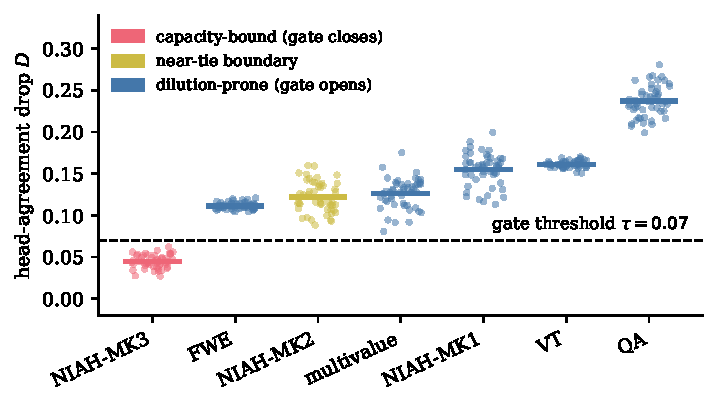
\includegraphics[width=0.60\linewidth]{figs/head_agreement_phenomenon.pdf}
  \caption{The head-agreement drop $D$ separates the two task classes
  (Qwen2.5-1.5B, RULER 4K, $N = 50$ per task; each dot is one input, bars
  are per-task means). NIAH-MK3, the capacity-bound task, sits below the
  gate threshold $\tau = 0.07$; the dilution-prone tasks sit above it. The
  near-tie NIAH-MK1/MK2 tasks fall on the boundary, tracking the
  distractor-count gradient (App.~\ref{app:deferred}). The gate closes below
  the line (keep the full cache) and opens above it (run the base evictor).}
  \label{fig:phenomenon}
\end{figure}

\paragraph{Why this statistic?} Figure~\ref{fig:phenomenon} shows $D$
separating the capacity-bound anchor from the dilution-prone tasks at the
single threshold the gate uses. A same-inputs ablation against five other
cheap prefill statistics shows that $D$ is the only one that separates the
capacity-bound anchor, with per-input AUC $1.000$; every alternative fails
task-level separation and tops out at AUC $0.805$. The full ablation and
Table~\ref{tab:signal-ablation} are deferred to Appendix~\ref{app:deferred}.

\subsection{The headline result: $4 \times 4$ method-agnostic matrix}
\label{subsec:matrix}

The wrapper is orthogonal to base-evictor choice. Table~\ref{tab:matrix} reports
the $4 \times 4$ matrix of four base evictors (SnapKV, H2O, StreamingLLM,
PyramidKV) and four models, using the same gate and the same $\tau = 0.07$ with
no per-method tuning. Each $\Delta$ is gated minus plain accuracy, averaged over
eight budgets on the mixed suite (NIAH-MK3 + VT + FWE + QA\_1).

\begin{table}[t]
\centering
\caption{Headline $4 \times 4$ method-agnostic matrix. Same gate ($D \ge \tau$,
$\tau = 0.07$), same calibration, no per-base-evictor tuning. Every one of $16$
cells is positive; grand mean across the matrix is $+22.9$pp. The Qwen2.5-3B
SnapKV cell was executed at $\tau = 0.04$ and is reported here at
$\tau = 0.07$ via exact post-hoc re-evaluation (Appendix~\ref{app:repro});
all other cells were executed at $\tau = 0.07$.}
\label{tab:matrix}
\begin{tabular}{lcccccccc}
\toprule
 & \multicolumn{2}{c}{SnapKV} & \multicolumn{2}{c}{H2O} & \multicolumn{2}{c}{StreamingLLM} & \multicolumn{2}{c}{PyramidKV} \\
\cmidrule(lr){2-3}\cmidrule(lr){4-5}\cmidrule(lr){6-7}\cmidrule(lr){8-9}
Model & plain & gated & plain & gated & plain & gated & plain & gated \\
\midrule
Qwen2.5-1.5B & 0.438 & 0.559 & 0.196 & 0.357 & 0.033 & 0.195 & 0.417 & 0.570 \\
$\Delta$      & \multicolumn{2}{c}{$\!+\!0.121$} & \multicolumn{2}{c}{$\!+\!0.162$} & \multicolumn{2}{c}{$\!+\!0.163$} & \multicolumn{2}{c}{$\!+\!0.152$} \\
\midrule
Qwen2.5-3B   & 0.580 & 0.839 & 0.339 & 0.642 & 0.052 & 0.482 & 0.536 & 0.865 \\
$\Delta$      & \multicolumn{2}{c}{$\!+\!0.259$} & \multicolumn{2}{c}{$\!+\!0.303$} & \multicolumn{2}{c}{$\!+\!0.430$} & \multicolumn{2}{c}{$\!+\!0.329$} \\
\midrule
Qwen2.5-14B  & 0.709 & 0.853 & 0.668 & 0.868 & 0.080 & 0.330 & 0.632 & 0.860 \\
$\Delta$      & \multicolumn{2}{c}{$\!+\!0.143$} & \multicolumn{2}{c}{$\!+\!0.200$} & \multicolumn{2}{c}{$\!+\!0.250$} & \multicolumn{2}{c}{$\!+\!0.228$} \\
\midrule
Mistral-7B    & 0.623 & 0.810 & 0.400 & 0.636 & 0.102 & 0.365 & 0.593 & 0.823 \\
$\Delta$      & \multicolumn{2}{c}{$\!+\!0.187$} & \multicolumn{2}{c}{$\!+\!0.236$} & \multicolumn{2}{c}{$\!+\!0.263$} & \multicolumn{2}{c}{$\!+\!0.231$} \\
\bottomrule
\end{tabular}
\end{table}

Cross-architecture SnapKV-only runs on two Llama-family models
(Yi-1.5-9B, Llama-3.1-8B; Table~\ref{tab:crossarch}), a scale-validation
run at 32B, a best-plain-vs-best-gated comparison
(Table~\ref{tab:bestplain}) that rules out ``you only beat the weakest
baseline,'' and a discussion of why the deltas vary across base evictors
are all deferred to Appendix~\ref{app:deferred}.

The clearest single result is on Mistral 4K NIAH-MK3, where the gate holds
accuracy flat as plain SnapKV collapses to zero
(Figure~\ref{fig:mistral-showcase}, quantified in Section~\ref{sec:experiments}).

A bar-chart rendering of the headline matrix (Figure~\ref{fig:matrix}) and
a composition test against a fifth, geometry-based (ManifoldKV-style) base
evictor, which the same gate lifts by $\Delta = +16.2$pp and which shows
composition extends outside the attention-score family, are deferred to
Appendix~\ref{app:deferred}.

\section{Calibration recipe}
\label{sec:recipe}

The fixed $\tau = 0.07$ mis-classifies only one of the eight
Qwen/Mistral (model, context) cells (Qwen2.5-3B 16K, where layer-bin
drops compress at long context). A one-shot, label-free $40$-input
recipe, which picks $20$ inputs from a capacity-bound task and $20$ from a
dilution-prone task and sets $\tau$ to the midpoint of their mean drops
(Eq.~\eqref{eq:tau}), fixes that failure cell, turning
$+3.4$pp into $+5.4$pp. An architecture-normalized variant needs
no task labels: standardizing the drop per model
($z$-scoring over an unlabeled $\sim 100$-input pilot) transfers a single
global threshold zero-shot to the two held-out Llama-family models
(Yi-1.5-9B, Llama-3.1-8B) and to Qwen3-4B, where the fixed $\tau$ fails
outright. Full recipe, $\tau$-sensitivity analysis, and the per-family
$z$-score results (Table~\ref{tab:recipe},
Figure~\ref{fig:tau-sensitivity}) are deferred to
Appendix~\ref{app:deferred}.

\section{Theory: the mechanism and the scaling formula}
\label{sec:theory}

We adopt verbatim the dilution mechanism from \citet{arxiv260509649},
which suffices to motivate our gating predictor: for a single attention
head reading a relevant set $\mathcal{R}$ and a noise set $\mathcal{N}$
with pre-eviction signal mass $\alpha_{\mathcal{R}}$, near-tie
distractors force the dilution $\delta_t$ (the attention mass outside the
useful set) to be large, and preferential retention reduces it. The
empirical partition follows: capacity-bound tasks concentrate a
single signal ($\alpha_{\mathcal{R}} \to 1$), while dilution-prone tasks spread
it ($\alpha_{\mathcal{R}} \ll 1$). Combining the head-SNR argument
with the accuracy headroom $1 - A_{\mathrm{full}}(M, T)$, the per-input
expected accuracy improvement at a single budget $b$ obeys the
context-length scaling formula

\begin{equation}
\label{eq:scaling}
\rho_{\mathrm{KV}}(\mathsf{T}, M, T) \;\approx\;
\bigl(1 - A_{\mathrm{full}}(M, T)\bigr) \cdot p_{\mathrm{recov}}\bigl(\rho_{\mathcal{R}} / \gamma\bigr),
\qquad p_{\mathrm{recov}}: [0, \infty) \to [0, 1],
\end{equation}

where $\rho_{\mathcal{R}}$ is the retained fraction of relevant mass and
$\gamma$ the noise-retention ratio. The full mechanism setup, the
derivation that the partition follows from it, the context-length-scaling
argument and its informal proposition, and the sufficient-condition bridge
from the observable head-agreement drop $D$ (Eq.~\eqref{eq:D}) to the
dilution $\delta_t$ (Eq.~\eqref{eq:bridge}) are deferred to
Appendix~\ref{app:deferred}, with the two proof sketches in
Appendices~\ref{app:proof-scaling} and~\ref{app:sufficient}.

\section{Experiments}
\label{sec:experiments}

\subsection{Setup}

Models, contexts, eviction policies, and protection settings are as in
Section~\ref{sec:partition}. The matrix uses RULER 4K with the four-task
mixed suite (NIAH-MK3 + VT + FWE + QA\_1, $N = 100$ each), as RULER 4K
fits in one A100 80GB at all four base evictors and four models. The
scaling table uses 4K and 16K. The gate cost is reported on Qwen2.5-1.5B
4K and extrapolates linearly.

\paragraph{Uncertainty quantification.} All gating deltas carry $95\%$
cluster-bootstrap confidence intervals over inputs and all recovery rates
$\rho$ Wilson score intervals; every one of the $16$ matrix deltas is
positive with its entire interval above zero (smallest lower bound $+9.3$pp),
the sole exception being the Qwen2.5-3B 16K gate-misfire cell, and the
partition claim rests on the unambiguous pooled NIAH-MK3 contrast ($2/526$
inputs recover). The full bootstrap protocol and per-cell interval discussion
are deferred to Appendix~\ref{app:deferred} and Appendix~\ref{app:ci}.

The Qwen2.5-3B 4K SnapKV cell decomposed along the budget axis
(Table~\ref{tab:qwen3b-curve}) and the 8-cell cross-(model, context)
scaling table (Table~\ref{tab:scaling}, whose pattern matches the
context-length scaling formula) are deferred to
Appendix~\ref{app:deferred}.

\subsection{A pre-registered out-of-range test at 32K}
\label{subsec:prereg32k}

All scaling-formula evidence so far is in-range (4K/16K). We therefore
ran a pre-registered extrapolation test: fit the per-task recovery
ratio $\rho / (1 - A_{\mathrm{full}})$ on the existing 4K/16K cells
only, measure $A_{\mathrm{full}}$ at 32K (Qwen2.5-1.5B, $N = 100$ per
task, RULER-32K with the Qwen2.5 tokenizer), freeze and hash the
predicted $\rho$ intervals \emph{before} running any eviction budget,
then sweep. The timestamped protocol log and the frozen prediction
file's SHA-256 ship with the released logs. The full prediction-vs-measurement
table (Table~\ref{tab:prereg32k}) is deferred to Appendix~\ref{app:deferred}.

One of three predictions lands strictly inside its interval
(Table~\ref{tab:prereg32k}). Both
misses are in the same direction: \emph{more} recovery than
predicted. VT's measured ratio ($0.74$) exceeds every in-range ratio
($\max 0.56$): recovery per unit headroom grows with context rather
than staying constant, and at 32K eviction beats the full cache on VT
in \emph{mean} accuracy, not just per input ($0.850$ at $b = 0.125$
vs.\ $0.810$ full-KV), the strongest dilution signature in any cell we
measured. FWE lands, but its ratio ($0.10$) matches the 1.5B in-range
cells rather than the pooled band, i.e., the FWE ratio is
model-dependent. MK3's point estimate slips above the $0.02$ pin
(Wilson CI still covers it), while the partition itself sharpens: the
MK3 recovery ratio ($0.047$ at headroom $0.86$) is $15\times$ below
VT's ($0.74$ at headroom $0.19$). Net reading: the formula's
\emph{directional} content ($\rho$ tracks headroom, and the
partition is visible in the ratio at any context length) survives
out-of-range, but the constant-ratio proportionality does not: the
dilution-side ratio grows with context and varies by (task, model). We
accordingly claim the formula as a directional and ordinal law, not a
quantitative one.

\subsection{The accuracy--memory frontier}
\label{subsec:pareto}

\begin{figure}[t]
  \centering
  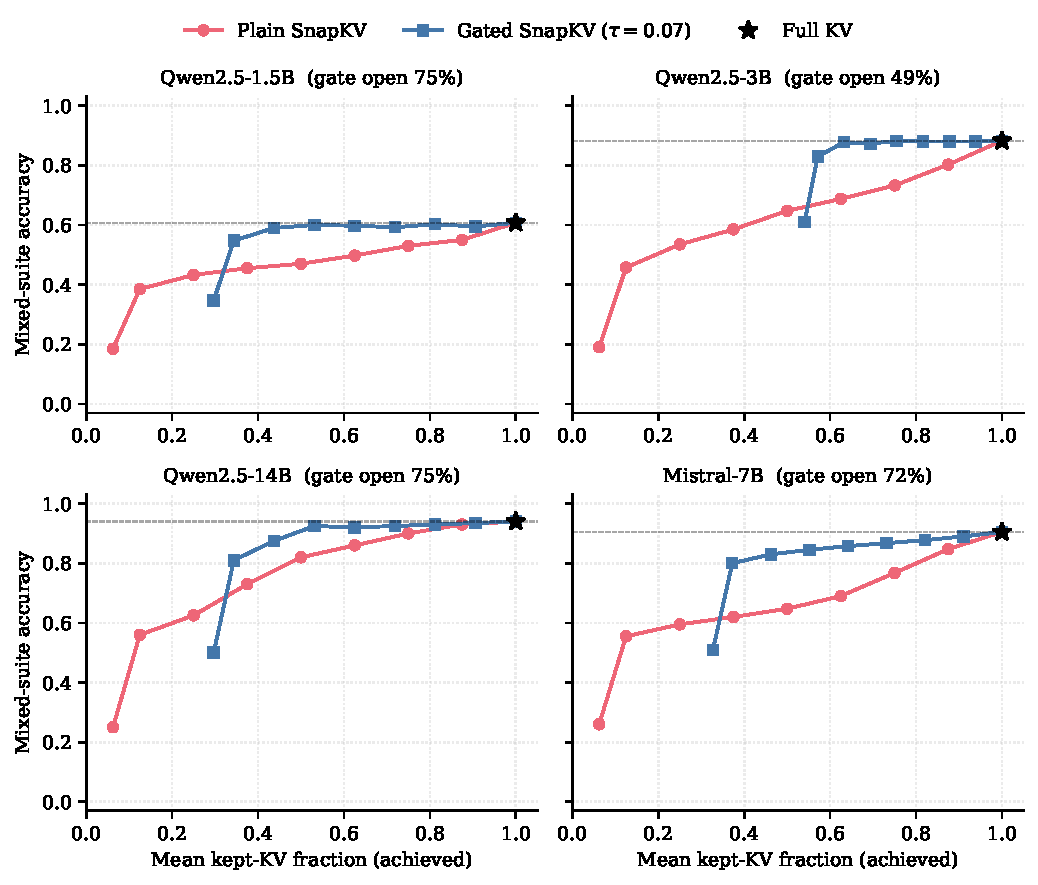
\includegraphics[width=0.78\linewidth]{figs/pareto_gated.pdf}
  \caption{Accuracy vs.\ \emph{achieved} kept-KV fraction (mean over inputs of
  $n_{\text{kept}}/T$) on the mixed 4K suite (NIAH-MK3 + VT + FWE + QA\_1),
  SnapKV. Because the gate falls back to the full cache when it closes, gated
  points sit at larger kept-KV than their nominal budget; the honest comparison
  is at matched achieved cache size. For every target kept-KV fraction
  $\gtrsim 1/3$ (Qwen3B: $\gtrsim 0.57$) the gated curve is the Pareto
  frontier, by up to $+19$pp over plain at equal cache size; at the most
  aggressive nominal budget ($b=0.0625$, leftmost gated point) the gated point
  is dominated by plain eviction at a matched cache size, and $\tau=0.07$
  caps achievable compression at $1-\text{open-fraction}$ of the cache
  ($0.25$--$0.51$ across models). All gated results use the post-hoc
  $\tau=0.07$ reconstruction (Appendix~\ref{app:repro}); the reconstruction
  reproduces the stored gated outcomes exactly on the three runs executed at
  $\tau=0.07$.}
  \label{fig:pareto-gated}
\end{figure}

\paragraph{What cache size does the gate actually deliver?}
Because the gate keeps the full cache when it closes, the two arms hold
different amounts of cache at the same nominal budget. Re-plotting accuracy
against \emph{achieved} kept-KV (Figure~\ref{fig:pareto-gated}) shows that
gating is not a free win everywhere but a strict improvement of the
accuracy--memory frontier over a wide range: for any target cache size above
roughly one third of full KV, gating delivers $3$--$19$pp higher accuracy than
plain SnapKV at the \emph{same} achieved kept-KV on all four models, and below
that range it saturates by design (the gate's full-KV fallback bounds
compression at $1-p_{\text{open}}$). At the aggressive operating point the
deployment delivers $3.1$--$3.4\times$ memory reduction ($1.8\times$ on
Qwen-3B), and against a per-input oracle the gate recovers a mean $69\%$ of the
available headroom, almost all of it task-level protection of the
capacity-bound anchor. The achieved-compression breakdown
(Table~\ref{tab:achieved-compression}), the exact frontier mechanics, and the
oracle-gap per cell are deferred to Appendix~\ref{app:deferred}.

\paragraph{Drop ordering and scaling-formula check.} The head-agreement
drop orders the tasks the same way in every Qwen and Mistral cell
(NIAH-MK3 smallest; Figure~\ref{fig:phenomenon} shows one cell), fully
preserved on Qwen/Mistral and partially on the Llama family
(Table~\ref{tab:drops}, App.~\ref{subsec:drops-ordering}). Verifying
Eq.~\eqref{eq:scaling} on the 4K/16K cells, the ratio
$\rho / (1 - A_{\mathrm{full}})$ clusters in $[0.25, 0.55]$ on
dilution-prone tasks and stays $\le 0.02$ on NIAH-MK3 regardless of
headroom. Both the drop table and the scaling verification
(Table~\ref{tab:scaling-formula}, Figure~\ref{fig:scaling}) are in
Appendix~\ref{app:deferred}.

\subsection{Single-task showcase: Mistral 4K NIAH-MK3}

The strongest single-task win (Figure~\ref{fig:mistral-showcase}). $N = 100$.
Plain SnapKV at $b = 0.0625$
collapses from $0.99$ full-cache to $0.00$; gated SnapKV holds $0.89$
across all budgets. The gate is closed on $90/100$ inputs (correct
prediction of capacity-bound) with $10/100$ false positives (gate
opens, eviction destroys the needle).

\begin{figure}[t]
\centering
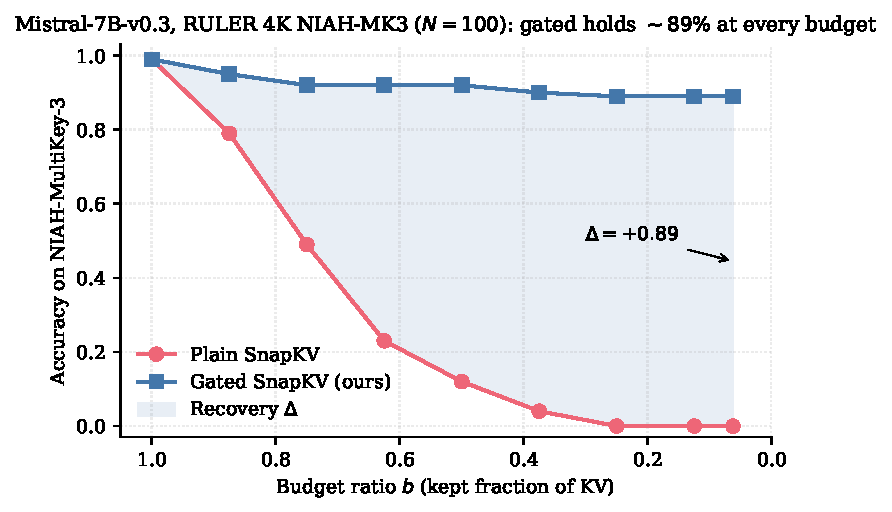
\includegraphics[width=0.54\textwidth]{figs/mistral_niah_showcase.pdf}
\caption{Mistral-7B 4K NIAH-MK3, $N = 100$. Accuracy vs.\ KV
budget for plain SnapKV (solid, collapses to $0$) and gated SnapKV
(dashed, $0.89$ flat across budgets). The gate prevents the collapse
without retraining the base evictor or seeing labels.}
\label{fig:mistral-showcase}
\end{figure}

\subsection{Cost of the gate, and what the deployment delivers}
\label{subsec:cost}

The gate costs $17$ms on Qwen2.5-1.5B and $89$ms on Mistral-7B and
yields a $1.29\times$ decode speedup at 7B; the full end-to-end
efficiency table (Table~\ref{tab:latency}), the per-layer ablation, and
the random-eviction control are deferred to Appendix~\ref{app:deferred}.

\subsection{Head-to-heads with published methods}
\label{subsec:capkv-longbench}
\label{subsec:dbtrimkv}

The gate wraps published evictors, not just the base four. Around a
re-implementation of CapKV~\citep{arxiv260425975} on LongBench (Qwen2.5-3B,
$b = 0.5$) it is weakly positive at matched budget ($+1.5$pp qasper, $+8.3$pp
triviaqa, concentrated on the gate-closed subset). Around the pretrained
trained-gate evictor DBTrimKV~\citep{arxiv260509649} (Qwen3-4B-Instruct-2507,
RULER 4K) it improves matched-budget accuracy by $+23.3$pp overall,
concentrated on capacity-bound NIAH-MK3 ($+53.3$pp) as the mechanism predicts;
at the fixed $\tau = 0.07$ the gate fires on only $1.7\%$ of Qwen3 records, so
this is a quality win dominated by the full-KV fallback, and the per-model
z-scored threshold restores a compressing gate. Both tables
(\ref{tab:capkv}, \ref{tab:dbtrimkv}) and details are in
Appendix~\ref{app:deferred}.

\section{Limitations}
\label{sec:limitations}

We list the limitations of the present work in roughly decreasing
order of severity.

\paragraph{The theory holds under named assumptions, not unconditionally.}
On the single-head surrogate we prove both directions of the bridge
between the head-agreement drop $D$ and the dilution $\delta_t$ of
\citet{arxiv260509649}: the sufficient direction (Appendix~\ref{app:sufficient})
and, sharpened in Appendix~\ref{app:sharpened}, the exact leading constant of
the scaling law (a two-sided bound, no budget-grid factor), the converse
``capacity-bound $\Rightarrow$ small $D$'' under an explicit margin-to-noise
assumption, and an $O(H^2\varepsilon)$ approximate form of the useful-set
identification (A4). What remains unproven is that real attention weights
satisfy those named assumptions (the margin-to-noise ratio, the
consensus-usefulness inclusion); we test them only through their consequences
(small $D$ on NIAH-MK3 in every cell). The empirical fallbacks, the partition
(Section~\ref{sec:partition}) and the orthogonality demonstration
(Section~\ref{subsec:matrix}), do not depend on the bridge.

\paragraph{The fixed $\tau$ does not transfer to the Llama family.} On
Yi-1.5-9B and Llama-3.1-8B, niah\_multivalue drops below $\tau = 0.07$
on both models; on Yi the gate additionally stays closed on FWE and VT
(gate-open fractions $0.00$ and $0.10$), and on Llama the
capacity-bound anchor NIAH-MK3 has mean $D = 0.073$, marginally
\emph{above} $\tau$, rescued only by per-input dispersion. The
accuracy deltas remain positive on both models, but on Yi that is
because the conservative full-KV fallback happens to fire where plain
SnapKV collapses, and the drop-vs-$\rho$ prediction itself is inverted
there. What transfers to the Llama family is the ordering, not the raw
threshold. The z-scored variant (Section~\ref{sec:recipe}) repairs
this with an unlabeled per-model pilot, lifting Llama $\Delta$ to
$+0.174$ and letting Yi compress at $\Delta = +0.145$; but it
adds a calibration step, its task-level claim excludes
niah\_multivalue, and per-input separation on the Llama family remains
imperfect (AUC $\approx 0.80$). A per-input statistic beyond mean $D$
is the natural follow-up.

\paragraph{``Capacity-bound'' is defined relative to the scorer being
gated.} The gate's job is to protect against the specific evictor it
wraps, so a task is capacity-bound for a scorer when that scorer cannot
retain the answer under compression. All four matrix base evictors score
positions by attention statistics, and NIAH-MK3 is capacity-bound for
them. It need not be capacity-bound for every scorer:
ManifoldKV~\citep{arxiv260208343} reports that a Euclidean-outlier key
scorer improves NIAH-MultiKey retention at $50\%$ compression. We make no
claim that NIAH-MK3 is un-compressible by any scorer; we claim the gate
correctly protects the scorer it wraps, and that it composes with a
geometry scorer ($+16.2$pp, Appendix~\ref{app:deferred}). We tested this
directly: a faithful per-layer geometry scorer (independent per-layer keep-sets)
also collapses on NIAH-MK3 in our harness, from $0.65$ full-cache accuracy to
$0.03$ at $50\%$ compression, below SnapKV. We could not reproduce ManifoldKV's
reported rescue, most likely because our RULER NIAH-MK3 and small model differ
from their setup; we do not dispute their number on their setup. NIAH-MK3 is
thus capacity-bound for every scorer we tested, which is the condition the gate
needs.

\paragraph{Single-seed runs; some cells are low-powered.} All sweeps
use greedy decoding and a single fixed seed; per-cell $N$ ranges from
$30$ to $100$ inputs (per-task $N$ noted in each table). All headline
deltas carry cluster-bootstrap $95\%$ intervals and all $\rho$ values
Wilson intervals (Section~\ref{sec:experiments},
Appendix~\ref{app:ci}); every matrix delta excludes zero, but the
per-cell partition calls are individually low-powered (most straddle
the $0.05$ threshold), and small-$N$ cells (Qwen-14B 16K, $N = 30$;
triviaqa head-to-head, $N = 24$) remain noisy. The partition claim
rests on the pooled contrast, which is unambiguous.

\paragraph{LongBench-SnapKV shows $\Delta \approx 0$ on the
dilution-prone subset.} On LongBench~\citep{arxiv230814508} qasper,
triviaqa, trec, and multifieldqa\_en under SnapKV scoring (plus
passage\_retrieval\_en on the 1.5B model), the pooled gated $\Delta$ is
within $\pm 1$pp of plain on all four models (Qwen2.5-1.5B $0.000$,
Qwen2.5-3B $+0.002$, Mistral-7B $+0.003$, Qwen2.5-14B $-0.008$). The
worst per-task cell is Qwen2.5-14B trec at $-2.2$pp, the only negative
gating result in the project, which we attribute to gate misfires on a
task with no capacity-bound inputs to rescue. LongBench, on this
subset, has no capacity-bound task; the partition predicts neutrality
and we observe it, including its mildly negative tail. The
complementary capacity-bound-minority behaviour
is documented in Section~\ref{subsec:capkv-longbench}.

Three further limitations are deferred to Appendix~\ref{app:deferred}: the
DBTrimKV head-to-head runs on Qwen3
rather than Qwen2.5, the matrix covers $4$ training-free base evictors
rather than $6$, and the only confirmed capacity-bound exemplar is
RULER NIAH-MK3 (LongBench passage\_count is a documented gate false positive;
Section~\ref{sec:limitations}).

\section{Conclusion}
\label{sec:conclusion}

The benefit of KV-cache eviction is not uniform across inputs; it is
sharply partitioned. The early-to-late head-agreement drop is a
$17$--$89$ms label-free statistic that predicts which side an input
falls on, and a gating wrapper turns the prediction into a
training-free policy: keep the full cache when the drop is small, run
the base evictor when it is large. The wrapper is positive on every
(model, base evictor, context) cell tested with a single threshold
$\tau = 0.07$, and the worst single-task failure of plain SnapKV we
observed (Mistral-7B NIAH-MK3, $99\% \to 0\%$ as budget shrinks)
becomes a flat $89\%$ under the gate.

Two questions remain open and we name them so the next paper does not
re-derive them. First, the bridge from the head-agreement drop to
the dilution $\delta_t$ is sketched in Appendix~\ref{app:sufficient}
on a single-head surrogate; the constants and the converse direction
on real multi-head attention are not formally proven. Second, the
Llama-architecture family mis-classifies niah\_multivalue at our
fixed $\tau$, suggesting that the early-vs-late layer-bin choice may
need to be model-family-specific for a fully cross-architecture
deployment. Both have natural attack paths laid out in the gap list
of Appendix~\ref{app:sufficient} and the limitations of
Section~\ref{sec:limitations}.

The mechanism is inherited from \citet{arxiv260509649}; the partition,
the predictor, the wrapper, and the joint $(M, T)$ scaling formula are
new.

\subsection*{Reproducibility statement}

All experiments run on single NVIDIA A100 80GB GPUs with PyTorch 2.11,
Transformers 5.9, and Python 3.13, in bfloat16 with greedy (argmax)
decoding, \texttt{max\_new\_tokens} $= 128$, and a fixed seed. Models
are the public Hugging Face checkpoints of Qwen2.5-1.5B/3B/14B-Instruct,
Mistral-7B-Instruct-v0.3, Yi-1.5-9B-Chat, and Llama-3.1-8B-Instruct;
tasks come from the \texttt{simonjegou/ruler} port of RULER and from
LongBench. Cache slicing preserves RoPE alignment via explicit
\texttt{position\_ids}; 16K runs use SDPA prefill with an eager
re-forward of the $w = 32$ observation window for scoring
(Appendix~\ref{app:repro}). Per-cell sample sizes are stated in each
table caption. The gate is one thresholded scalar (Eq.~\eqref{eq:D}),
so every gated number in the paper can be recomputed from the released
per-input logs; code, sweep configurations, and raw per-input jsonl
outputs will be released with the camera-ready.

\subsection*{Ethics statement}

This work studies inference-time efficiency of publicly released
language models on public benchmarks. It involves no human subjects,
no personal data, and no new model training. Better KV-cache eviction
lowers the memory and energy cost of long-context inference; we see no
ethical risk specific to this method beyond those of the underlying
models.

\bibliographystyle{iclr2026_conference}
\bibliography{../main}

\appendix

\section{Deferred tables, derivations, and secondary experiments}
\label{app:deferred}

% DEFERRED-CONTENT-START

\subsection{Related work (full treatment)}

\paragraph{Five close concurrent neighbors.}
\citet{arxiv260509649} (DBTrimKV) is the most important reference point.
Their Proposition~3.1 establishes that near-tie distractors force attention
dilution in a single head, and Corollary~3.2 shows preferential retention of
high-attention positions reduces it; Section~\ref{sec:theory} adopts this
mechanism. Their evaluation reports DBTrimKV $>$ full-cache on multi-turn
dialogue but does not characterise a task family on which their method
underperforms full-cache. They train a retention gate end-to-end; our gate is
label-free and wraps theirs (and any other) without retraining. Direct
head-to-head: Section~\ref{subsec:dbtrimkv}, $\Delta = +0.233$ at matched
budget on RULER 4K Qwen3-4B-Instruct.

\citet{arxiv260425975}
(CapKV) derives a closed-form, label-free eviction score from an
information-bottleneck objective and reports gains over a Vanilla baseline on
LongBench. Their score is task-agnostic; we partition tasks into a class for
which any eviction is risky and a class for which it helps, and report a
direct head-to-head wrapping CapKV in our gate
(Section~\ref{subsec:capkv-longbench}, $\Delta = +1.5$ to $+8.3$pp at
matched budget on two LongBench subtasks).

\citet{arxiv241214838}~(DynamicKV) introduces task-aware per-layer adaptive
budgets and explicitly observes that the layer-wise attention pattern
differs across task families, using attention statistics to drive a
continuous per-task budget allocation. This is the closest conceptual
neighbor to our partition: both detect that task type modulates which KV
positions matter. The differences are (i) DynamicKV's per-task budget is
fitted per task with calibration data; ours is a per-input gate triggered
by a single observable statistic with one fixed threshold; (ii) their
benchmark suite (LongBench) does not include a task on which eviction
strictly damages accuracy, so the binary partition is not visible in their
results; (iii) DynamicKV does not formalise a partition predictor or
attempt cross-architecture transfer. We therefore see our partition + drop
predictor + binary gate as orthogonal but partially overlapping with their
empirical observation, and we acknowledge the overlap.

\citet{arxiv260518053}~(``Protection Is All You Need'')
shows that structural protection (sink tokens plus a recent-token window)
dominates the choice of scorer on globally capacity-capped harnesses. Our
experimental setup uses protection of the same kind but smaller extent
($n_{\text{sink}} = 4$ sink tokens and a $w = 32$ observation window, versus
the $10\%$ prefix plus $10\%$ suffix they advocate). A protection-matched
ablation at their $10\% + 10\%$ setting confirms the partition is not an
artifact of light protection: NIAH-MK3 still collapses and the
eviction-helps signal survives (Section~\ref{sec:partition}).

\citet{arxiv260525475}~(IndexMem) trains a learnable indexer
plus latent memory and observes an information-density effect on LongBench
averages around 50\% compression. The benchmark-average hides which sub-tasks
contribute the peak; our partition makes that explicit, and our predictor is
training-free.

\paragraph{Concurrent 2026 diagnostics and wrappers.}
\citet{arxiv260508234} ask a similar headline question (when does value-aware
KV eviction help?). The clearest separation is the axis: their score is
\emph{value-aware} (a per-input support-coupling score $\phi(x)$ over value
states), whereas our signal is \emph{attention topology}, a complementary
account in the same sense that VaSE is (below). Their unit of analysis is the
selector rather than the task, their $\phi(x)$ drives diagnostic grid splits
rather than an evict-or-not gate, and they report that diagnostic signals
transfer across selectors only conditionally, which makes the single
transferred threshold we report non-obvious. \citet{arxiv251000231} document
instruction-type-dependent degradation under five eviction methods (some
instruction types become entirely ignored), the closest published task-level
failure taxonomy; we cede the hurts-degradation observation to them and claim
the joint helps-versus-hurts partition plus the a-priori predictor.
\citet{arxiv260301426} compute a \emph{within-layer} head-consensus level (how
much heads inside a layer attend to the same tokens) and relate it descriptively
to compression tolerance at the architecture level. Our statistic is different:
an \emph{early-to-late, cross-layer} drop in the top-$k$ agreement between heads,
computed online at prefill and thresholded per input to gate. To our knowledge
the identical statistic has not been proposed as an eviction gate; the ablation
of Appendix~\ref{app:deferred} shows it separates the partition cleanly (AUC
$1.000$) and transfers across families. On the failure side,
\citet{arxiv260603928}~(VaSE) trace catastrophic eviction failures to
high-magnitude value states, an axis orthogonal to our attention-topology
account, and ManifoldKV~\citep{arxiv260208343} shows that a Euclidean-outlier
key scorer improves NIAH-MultiKey retention under compression, which is why we
define ``capacity-bound'' relative to the scorer being gated
(Section~\ref{sec:limitations}). On the wrapper side,
VECTOR~\citep{arxiv260523258} and CriticalKV~\citep{arxiv250203805} are
plug-and-play augmentations over multiple base evictors; both always compress
under a fixed budget and adapt \emph{which} tokens are kept, whereas our gate
decides \emph{whether} to evict at all. Cross-family transfer of an eviction
control is itself known, via CompilerKV's~\citep{arxiv260208686} portable
per-head retention tables; we transfer one threshold instead, fixed across the
Qwen and Mistral families and extended to the Llama family and Qwen3 by an
unlabeled per-model standardization. Further concurrent evictors and allocators,
EntropyInfer~\citep{arxiv260609508},
CompressKV~\citep{arxiv260624467}, MomentKV~\citep{arxiv260601563},
EpiKV~\citep{arxiv260626472}, DefensiveKV~\citep{arxiv251013334}, and
TAKE~\citep{take-openreview}, adapt
budgets or scores per head, layer, token, or task, but none gates the eviction
decision per input or identifies a task class where eviction hurts
monotonically. Learned gates (Attention-Gate~\citep{arxiv241012876}, Fast
KVzip~\citep{arxiv260117668}) share the ``gate'' name but train their gating
parameters, unlike our inference-time scalar.

\paragraph{Older anchors.}
SnapKV~\citep{arxiv240414469}, H2O~\citep{arxiv230614048},
StreamingLLM~\citep{arxiv230917453}, PyramidKV~\citep{arxiv240602069}, and
Ada-KV~\citep{arxiv240711550} are the standard
training-free eviction baselines. We use SnapKV-style scoring as the base for
our gate and demonstrate orthogonality on H2O, StreamingLLM, and PyramidKV.
ForesightKV~\citep{arxiv260203203} and Learning-to-Evict~\citep{arxiv260210238}
train predictors of future utility; they require labels or rollouts. UT-ACA~%
\citep{arxiv260318446} and LU-KV~\citep{arxiv260208585} are calibration-based
context allocators on a single substrate. None proposes a binary task-type
partition or an a priori predictor.

\paragraph{Adjacent.}
AdaCompute-GBM~\citep{arxiv260414853} adapts on the self-consistency sample-count
axis; BudgetThinker~\citep{arxiv250817196} on the CoT chain-length axis;
LaTER~\citep{arxiv260507315} on latent-then-explicit reasoning. These work on
substrates orthogonal to the KV-cache axis we study.

\subsection{Additional empirical-partition analyses}

\paragraph{Qwen2.5-14B: re-entry to the dilution regime at long
context.} At 4K, three dilution-prone tasks (VT, FWE, QA\_2) sit at
$\rho \approx 0$: saturation, since $A_{\mathrm{full}} \in [0.92,
1.00]$ leaves no headroom for recovery, as Eq.~\eqref{eq:scaling}
predicts. At 16K, two of five dilution-prone tasks cross the
threshold (FWE $0.00 \to 0.20$, QA\_1 $0.06 \to 0.10$),
niah\_multivalue stays above it ($0.08 \to 0.07$), and the capacity-bound
NIAH-MK3 stays at exactly $0.00$ at both scales. VT ($0.00 \to 0.03$) and QA\_2
($0.02 \to 0.03$) remain below threshold because the inputs that the
model gets wrong at 4K stay wrong at every budget at 16K. Headroom
opens, dilution returns, NIAH-MK3 stays pinned: the partition behaves
as the scaling formula dictates, not as task identity dictates.

\paragraph{The partition is not a task-name heuristic.} The NIAH family contains
structurally different sub-tasks: niah\_multivalue (one key, many values) is
dilution-prone in seven of the eight cells measured (Table~\ref{tab:partition}), while
NIAH-MK3 (three near-tie keys, one of which is the answer) is capacity-bound in
all of them, and the distractor sweep below places niah\_multikey\_1 (no
near-tie distractors) on the dilution-prone side as well. The
\emph{near-tie distractor} structure, not the surface task category, is what
matters, and the head-agreement drop in Section~\ref{subsec:algo} catches the
distinction. A non-RULER probe confirms this: LongBench
passage\_retrieval\_en (pick 1 of 30 paragraphs; $N = 100$,
Qwen2.5-1.5B, prompts 10--16K tokens) \emph{looks} NIAH-like but has no
near-tie distractors, and it is evict-robust in practice, accuracy
stays flat from $b = 1.0$ to $b = 0.0625$ ($0.29 \to 0.26$, $\rho =
0.01$), while its mean drop $D = 0.105$ sits squarely in the
dilution-prone cluster, so the gate opens on $100/100$ inputs. The
predictor gets the surface-similar, structurally different task right
a priori.

\paragraph{The partition survives Garcia-scale protection.}
\citet{arxiv260518053} argue that structural protection dominates scorer
choice, so we re-ran the Qwen2.5-1.5B 4K partition tasks with their
$10\%$ prefix $+$ $10\%$ suffix protection ($n_{\text{sink}} = w = 410$;
$N = 100$ per task). One accounting note: protection overrides the
budget, so all nominal $b \le 0.1875$ share an effective floor of $824$
kept tokens ($\approx 0.21$ of context). Under this heavy protection the
partition is unchanged. NIAH-MK3 still collapses ($0.65$ full-KV $\to
0.09$ at the floor, an $86\%$ relative loss despite the floor cache being
$3.3\times$ our light-protection cache at nominal $b = 0.0625$), so the
capacity-bound failure is not protection-fixable. The eviction-helps
signal survives on the dilution-prone side ($\rho$: FWE $0.06 \to 0.13$,
QA\_1 $0.08 \to 0.07$, VT $0.06 \to 0.03$; aggregate $0.077 \ge 0.05$),
and FWE's floor accuracy ($0.31$) exceeds its full-KV accuracy ($0.22$).
Heavy protection is also not free: protected VT drops to $0.00$ at the
floor while our light-protection run holds $0.75$ at nominal $b = 0.125$
protected prefix/suffix tokens crowd out the scorer-selected middle
tokens the task needs. Caveat: in our harness $w$ is both the recency
protection and the SnapKV scoring window, so this run is a
protection-heavy SnapKV variant rather than an exact replication of
their protocol.

\subsection{Headline matrix figure and a geometry-based base evictor}

\begin{figure}[t]
\centering
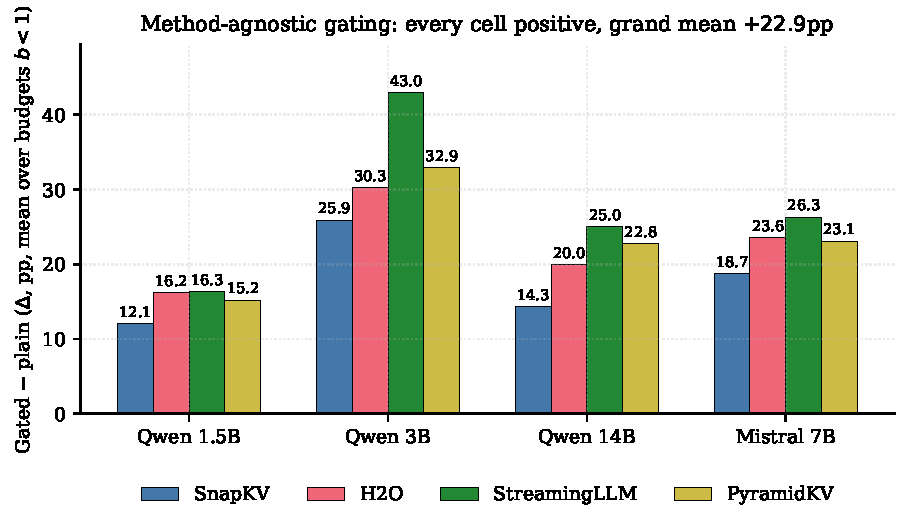
\includegraphics[width=0.95\textwidth]{figs/method_agnostic_matrix.pdf}
\caption{The headline $4 \times 4$ method-agnostic matrix.
Bars are gated $-$ plain accuracy averaged over budgets. The wrapper is positive
in every one of $16$ cells with a single $\tau = 0.07$ and no per-base-evictor
tuning. Grand mean $+22.9$pp.}
\label{fig:matrix}
\end{figure}

\paragraph{A fifth, geometry-based base evictor.} To test composition
beyond attention-score-based bases, we add a ManifoldKV-style
scorer~\citep{arxiv260208343}: per-(layer, head) Euclidean distance of
each key to the head's key centroid, averaged into a single shared keep
mask (a single-mask variant of their per-layer design, forced by our
uniform-cache harness). On the Qwen2.5-1.5B 4K mixed suite
($N = 100$/task, four budgets), the same gate at the same $\tau = 0.07$
lifts it by $\Delta = +16.2$pp with no negative (task, budget) cell; on
NIAH-MK3 the gate recovers full-KV accuracy ($0.00 \to 0.65$) at every
budget. Two observations: the gate signal is attention-based and
scorer-independent, so composition extends outside the attention-score
family; and our single-mask variant does \emph{not} reproduce
ManifoldKV's reported multi-key rescue (plain accuracy $0.01$ at
$b = 0.5$), their per-layer, per-head design may behave differently,
so we treat their published numbers as the authoritative claim and scope
ours accordingly (Section~\ref{sec:limitations}).

\subsection{Additional limitations}

\paragraph{Qwen2.5-3B 16K needs $\tau$-calibration.} The fixed
$\tau = 0.07$ default fails on this cell. The 40-input recipe of
Section~\ref{sec:recipe} fixes it ($\Delta$ goes from $+3.4$pp to
$+5.4$pp). We recommend the recipe as the deployment default; we keep
the fixed-$\tau$ result throughout to show the gap is small.

\paragraph{DBTrimKV head-to-head uses Qwen3 not Qwen2.5.} DBTrimKV's
pretrained gates exist only for Qwen3 variants, so
Section~\ref{subsec:dbtrimkv} runs on Qwen3-4B-Instruct-2507. The
matrix is Qwen2.5-keyed, so DBTrimKV stays a standalone head-to-head
rather than a matrix row.

\paragraph{4 base evictors, not 6.} The matrix covers training-free
policies. Trained / learned evictors (DBTrimKV, CapKV, IndexMem,
DynamicKV) are cited but not in the matrix for the codebase-compat
reason above.

\paragraph{The confirmed capacity-bound exemplar is RULER-only, and the gate
has a documented false positive.} Of our two non-RULER LongBench probes,
passage\_retrieval\_en is evict-robust and the gate correctly opens on it
(Section~\ref{sec:partition}).
NIAH-MK3 remains the only task where empirical capacity-boundedness (accuracy
collapse under eviction) and the gate's capacity-bound classification coincide.
Our second non-RULER probe is a genuine failure: on LongBench passage\_count at
Qwen2.5-14B, where full-KV accuracy clears floor ($0.16$ vs $0.04$ at 1.5B), the
gate closes on $95/95$ inputs (mean $D = -0.013 < \tau$), predicting
do-not-evict, yet eviction is empirically \emph{safe}: plain SnapKV accuracy is
statistically flat under $16\times$ eviction ($0.16 \to 0.13$, $12/15$
full-KV-correct inputs retained, $\rho = 0$). passage\_count is thus a
\emph{false positive} of the gate. This is the conservative dual of the MK2
boundary case (Section~\ref{sec:partition}): there the gate opens on an
empirically capacity-bound task; here it closes on an evict-safe one. The
failure direction is benign, an over-conservative gate costs compression, not
accuracy, but it shows the head-agreement drop is a one-sided predictor
(reliably firing on dilution-prone inputs) rather than a perfect classifier.
Multilingual and code tasks are out of scope; we expect the predictor to
transfer because the mechanism is architecture-level, not English-specific, but
we have not measured it.

\subsection{Mechanism-validation detail: distractor count drives $D$}

The RULER NIAH-MultiKey family lets us sweep the near-tie distractor count
directly: niah\_multikey\_1 (no distractors), niah\_multikey\_2 (one
near-tie distractor), niah\_multikey\_3 (two near-tie distractors).
The dilution mechanism of \citet{arxiv260509649} predicts that more
near-tie distractors should produce
larger expected dilution $\delta_t$ and (via App.~\ref{app:sufficient})
smaller head-agreement drop $D$. On Qwen2.5-1.5B at RULER 4K, $N = 50$
per task, we observe a clean monotone gradient (Table~\ref{tab:distractor}).

\begin{table}[t]
\centering
\caption{Distractor-count sweep on the NIAH-MultiKey family
(Qwen2.5-1.5B, RULER 4K, $N = 50$ per task). Mean head-agreement drop
$D$ shrinks monotonically as the near-tie distractor count grows.}
\label{tab:distractor}
\begin{tabular}{lccccc}
\toprule
Task & mean $D$ & gate-open frac & $\rho_{\mathrm{plain}}$ & $\rho_{\mathrm{gated}}$ & plain at $b{=}0.0625$ \\
\midrule
niah\_multikey\_1 & $+0.155$ & $1.00$ & $0.04$ & $0.04$ & $0.36$ \\
niah\_multikey\_2 & $+0.122$ & $1.00$ & $0.00$ & $0.00$ & $0.00$ \\
niah\_multikey\_3 & $+0.045$ & $0.00$ & $0.00$ & $0.00$ & $0.00$ \\
\bottomrule
\end{tabular}
\end{table}

$D$ shrinks by $\sim 3.5\times$ from $0 \to 2$ near-tie distractors,
and per-input ranges between MK2 and MK3 do not overlap
($\max_{\text{MK3}} D = 0.062 < \min_{\text{MK2}} D = 0.088$): the
partition predictor separates 2-distractor inputs from
$\leq 1$-distractor inputs $100\%$ of the time at $\tau = 0.07$. The
monotone gradient replicates on Mistral-7B-v0.3 ($D = 0.081, 0.072,
0.060$ for MK1/MK2/MK3, $N = 50$ per task), confirming the mechanism
is not Qwen-specific, though the finer per-input MK2/MK3 non-overlap is
(their ranges overlap on Mistral). On a
controlled sweep over distractor count, the head-agreement drop and
the partition track each other monotonically, exactly as the
$\delta_t$ dilution mechanism predicts.

\paragraph{The single-near-tie boundary case.} MK2 is empirically
capacity-bound at low budgets (plain SnapKV collapses from $80\%$ at
$b{=}1$ to $0\%$ at $b{=}0.0625$) yet is classified as dilution-prone
by the predictor at $\tau = 0.07$: MK2's mean $D = 0.122$ sits between
the MK3 cluster ($D \leq 0.062$) and the MK1 cluster ($D \geq 0.099$),
co-located with genuinely dilution-prone FWE ($D = 0.098$) and
niah\_multivalue ($D = 0.107$). No single mean-$D$ threshold separates
MK2 from the dilution-prone cluster on this model. The predictor
therefore falls back to its weakest form: it correctly classifies MK3
and the standard dilution-prone tasks but mis-classifies single-near-tie
MK2. Per-input recovery information beyond mean $D$ would be needed to
catch it at deployment.

\subsection{Gate-signal ablation: why the head-agreement drop}

A same-inputs ablation against five other
cheap prefill statistics (Table~\ref{tab:signal-ablation}; one shared
prefill per input, $N = 50$ per task across seven RULER tasks) shows $D$
is not merely the best candidate but the only one that separates the
partition at all: MK3's mean $D$ sits strictly below all four
dilution-prone task means with per-input AUC $1.000$, while every
alternative fails task-level separation and tops out at AUC $0.805$.
The dissection is informative: raw attention entropy is at chance
($0.508$), taking its early-vs-late layer contrast lifts it to $0.805$,
and replacing entropy with head \emph{agreement} makes the separation
exact, both the layer contrast and the agreement measure matter, with
agreement decisive. No alternative is even a redundant proxy (all
$|r|$ with $D \le 0.64$). Consistent with the MK2 boundary case of
Section~\ref{sec:partition}, extending the capacity-bound anchor to
MK3$+$MK2 breaks task-level separation for $D$ too (AUC $0.859$): $D$
tracks the near-tie distractor gradient, not a binary task label.

\begin{table}[t]
\centering
\caption{Gate-signal ablation on Qwen2.5-1.5B-Instruct (RULER 4K, $N=50$ per
task, one shared prefill per input). Each cheap prefill statistic is tested
for separating the capacity-bound anchor (NIAH-MK3, and MK3+MK2) from the
dilution-prone tasks (vt, fwe, qa\_1, multivalue). ``Sep.'' = a single
threshold puts the capacity-bound task mean(s) strictly on one side of all
four dilution task means; AUCs are per-input and oriented per signal
(0.5 = chance); ``MK mono.'' = task means are monotone along the
MK1$\to$MK2$\to$MK3 distractor gradient; $r$ = Pearson correlation with $D$.}
\label{tab:signal-ablation}
\resizebox{\textwidth}{!}{%
\begin{tabular}{lcccccc}
\toprule
Signal & Sep.\ MK3 & Sep.\ MK3+MK2 & AUC MK3 & AUC MK3+MK2 & MK mono.\ & $r$ w/ $D$ \\
\midrule
head-agreement drop $D$ (paper) & \yes & \no & \textbf{1.000} & \textbf{0.859} & \yes & $+1.00$ \\
mean attention entropy (norm.) & \no & \no & 0.508 & 0.670 & \no & $+0.08$ \\
top-32 attention mass share & \no & \no & 0.784 & 0.574 & \yes & $+0.22$ \\
max single-position share & \no & \no & 0.723 & 0.708 & \yes & $+0.32$ \\
key-norm dispersion (std/mean) & \no & \no & 0.570 & 0.560 & \no & $+0.01$ \\
early$-$late entropy drop & \no & \no & 0.805 & 0.575 & \no & $-0.64$ \\
\bottomrule
\end{tabular}%
}
\end{table}

\subsection{Cross-architecture, scale, and best-plain results}

\begin{table}[t]
\centering
\caption{Cross-architecture SnapKV-only runs on two Llama-family models.
These use the four most aggressive budgets $\{0.0625, 0.125, 0.25, 0.5\}$
rather than the eight-budget grid of Table~\ref{tab:matrix}, so the
$\Delta$ values are not directly comparable to the matrix rows
(aggressive-budget-only averaging inflates $\Delta$).}
\label{tab:crossarch}
\begin{tabular}{lccc}
\toprule
Model & plain SnapKV & gated SnapKV & $\Delta$ \\
\midrule
Yi-1.5-9B    & 0.464 & 0.854 & $+0.390$ \\
Llama-3.1-8B & 0.509 & 0.618 & $+0.109$ \\
\bottomrule
\end{tabular}
\end{table}

\paragraph{Yi-1.5-9B and Llama-3.1-8B cross-architecture runs
(Table~\ref{tab:crossarch}).} Yi
($\Delta = +39.0$pp) and Llama ($\Delta = +10.9$pp) are
Llama-architecture descendants distinct from Qwen and Mistral; only
the SnapKV column was run for compute, and on a smaller, more
aggressive budget grid (see caption). The sign is positive on both,
but on these two models part of the gain comes from the gate closing
conservatively on tasks where plain SnapKV collapses, rather than from
a correctly recovered partition. The per-task breakdown and the
shared Llama-arch family caveat (niah\_multivalue mis-classifies on
both Yi and Llama) are in Section~\ref{subsec:drops-ordering} and
Section~\ref{sec:limitations}.

\paragraph{Scale validation at 32B.} A SnapKV-only run on
Qwen2.5-32B-Instruct (RULER 4K mixed suite, $N = 100$) confirms the
predictor scales but also illustrates the saturation arm of the scaling
formula. The drop ordering transfers cleanly (NIAH-MK3 smallest at
$D = 0.025$, then FWE $0.052$, VT $0.079$, QA\_1 $0.103$). At the same
time the 32B model is near-saturated at 4K ($A_{\mathrm{full}} = 1.00$
on VT and NIAH-MK3, $0.93$--$0.94$ on FWE/QA\_1), so by
Eq.~\eqref{eq:scaling} there is essentially no dilution headroom and the
gate's value is capacity-bound protection rather than recovery: plain
SnapKV collapses at $b = 0.0625$ (NIAH-MK3 $0.00$, VT $0.00$, FWE
$0.09$) while the gate holds the full cache on the low-drop tasks,
giving mean $\Delta = +0.335$ at $\tau = 0.07$ (driven by NIAH-MK3
$+0.88$ and FWE $+0.44$) and $+0.237$ at the z-scored threshold with
more compression ($0.45$ vs.\ $0.63$ kept-KV). We report this as a
scale point for the partition and predictor, not as additional dilution
evidence.

\paragraph{Best plain vs.\ best gated.} A natural concern is ``you
only beat the weakest baseline.'' Comparing the best plain evictor against the
best gated evictor for each model rules this out (Table~\ref{tab:bestplain}).

\begin{table}[t]
\centering
\caption{Best plain evictor vs.\ best gated evictor per model, over
the four base evictors of Table~\ref{tab:matrix} at the same budget grid.}
\label{tab:bestplain}
\begin{tabular}{lccc}
\toprule
Model & Best plain & Best gated & $\Delta$ \\
\midrule
Qwen2.5-1.5B & 0.438 (SnapKV)    & 0.570 (PyramidKV) & $+0.132$ \\
Qwen2.5-3B   & 0.580 (SnapKV)    & 0.865 (PyramidKV) & $+0.285$ \\
Qwen2.5-14B  & 0.709 (SnapKV)    & 0.868 (H2O)       & $+0.159$ \\
Mistral-7B    & 0.623 (SnapKV)    & 0.823 (PyramidKV) & $+0.201$ \\
\bottomrule
\end{tabular}
\end{table}

\paragraph{Why the deltas vary across base evictors.} StreamingLLM keeps only
$36$ tokens regardless of budget; on the dilution-prone fraction it is near
zero plain, near zero gated, so gating contributes only via the gate-closed
NIAH-MK3 inputs that go from $0$ to full-KV accuracy. SnapKV is budget-scaled
and degrades more gracefully, so it has less room for gating to recover.
PyramidKV's depth-weighted scoring biases toward bottom layers but produces
similar absolute gains to SnapKV. The pattern is that gating $\Delta$ tracks how
much the base evictor collapses on the capacity-bound fraction. Two
implementation caveats: our PyramidKV is a depth-weighted variant of the
published per-layer budget schedule, and under two-pass prefill scoring
(used on Qwen2.5-14B for memory) the H2O score only sees the last $w$
queries, so the 14B H2O column degenerates toward SnapKV-style scoring; its
$\Delta$ there should be read as a near-duplicate of the SnapKV cell rather
than an independent base evictor.

\subsection{Calibration recipe details}

We provide a one-shot, label-free calibration recipe.

\paragraph{Recipe.} For a new (model, context):
\begin{enumerate}
  \item Pick $20$ inputs from a known capacity-bound task (NIAH-MK3) and
  compute the head-agreement drop $D_i$ on each. Average to get
  $\bar D_{\mathcal C}$.
  \item Pick $20$ inputs from a known dilution-prone task (VT) and compute
  $\bar D_{\mathcal D}$.
  \item Set
  \begin{equation}
  \label{eq:tau}
  \tau = \tfrac{1}{2}\bigl(\bar D_{\mathcal C} + \bar D_{\mathcal D}\bigr).
  \end{equation}
\end{enumerate}
$40$ prefills, no labels, no decode, $<5$ minutes on a single A100.

\paragraph{Validation.} On four cells (Table~\ref{tab:recipe}). The recipe
lifts Qwen2.5-3B 16K from $+3.4$pp to $+5.4$pp (the only failure cell turned
into a win) and lifts Mistral 4K from $+18.7$pp to $+22.3$pp. It is
neutral on average across the four cells but with smaller variance.

\begin{table}[t]
\centering
\caption{Calibration-recipe validation. $\bar D_{\mathcal C}$ uses NIAH-MK3
($N = 20$); $\bar D_{\mathcal D}$ uses VT ($N = 20$).
Bolded $\tau$-choice column is the winner per cell. The pilot means here
are computed on $20$-input samples and therefore differ slightly from the
$N \ge 50$ per-task means of Table~\ref{tab:drops}.}
\label{tab:recipe}
\begin{tabular}{lccccc}
\toprule
Cell & $\bar D_{\mathcal C}$ & $\bar D_{\mathcal D}$ & $\tau_{\mathrm{cal}}$
& gated@$\tau_{\mathrm{cal}}$ & gated@$\tau\!=\!0.07$ \\
\midrule
Qwen2.5-1.5B 4K & $+0.045$ & $+0.161$ & $+0.103$ & $+0.121$ & $+0.121$ \\
Qwen2.5-3B 4K   & $-0.002$ & $+0.076$ & $+0.037$ & $+0.213$ & $\boldsymbol{+0.259}$ \\
Qwen2.5-3B 16K  & $-0.021$ & $+0.068$ & $+0.024$ & $\boldsymbol{+0.054}$ & $+0.034$ \\
Mistral 4K       & $+0.060$ & $+0.096$ & $+0.078$ & $\boldsymbol{+0.223}$ & $+0.187$ \\
\bottomrule
\end{tabular}
\end{table}

\paragraph{$\tau$ sensitivity.} Sweeping $\tau \in \{0.01, 0.025,
0.04, 0.055, 0.07, 0.085, 0.10, 0.13, 0.16, 0.20\}$ on Qwen2.5-1.5B at
RULER 4K (mixed suite, $N=100$, budgets $\{0.5, 0.25, 0.125, 0.0625\}$,
SnapKV) shows an operational plateau $\tau \in [0.055, 0.10]$ inside
which $\Delta$ varies by under $1$pp and both false-positive (gate
fires on capacity-bound MK3) and false-negative (gate stays closed on
dilution-prone VT/FWE/QA\_1) rates stay at or below $9\%$. The deployed
$\tau = 0.07$ sits in the middle of this plateau
(Figure~\ref{fig:tau-sensitivity}); outside it the behavior changes
character (below $0.04$: FP $\geq 64\%$, $\Delta \leq +0.06$; above
$0.13$: FN $\geq 33\%$ and the method degenerates toward ``always full
KV,'' which on this full-KV-strong suite still yields a large $\Delta$
the sweep's raw maximum is in fact at $\tau = 0.20$, but at the
price of never compressing, so it is not a useful operating point). The
deployed threshold does not depend on a knife-edge.

\begin{figure}[h]
  \centering
  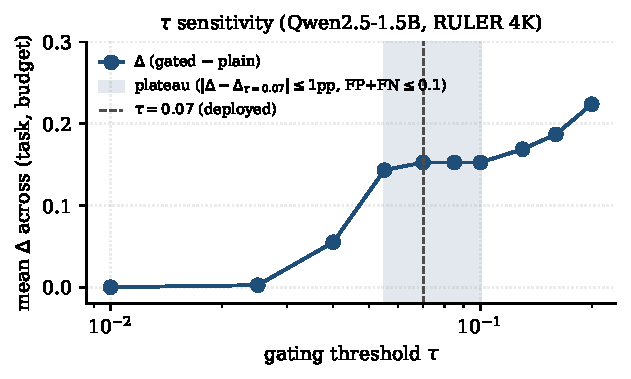
\includegraphics[width=0.62\linewidth]{figs/tau_sensitivity.pdf}
  \caption{$\tau$ sensitivity on Qwen2.5-1.5B, RULER 4K. Mean
  $\Delta$ (gated $-$ plain) over (task, budget) cells. Shaded band:
  operational plateau where $|\Delta - \Delta_{\tau=0.07}| \leq 1$pp
  and FP$+$FN $\leq 0.10$. The deployed $\tau = 0.07$ sits in the
  middle of the plateau.}
  \label{fig:tau-sensitivity}
\end{figure}

\paragraph{Architecture-normalized variant: the z-scored drop.} The recipe
above calibrates a per-cell threshold from two labeled pilot tasks. A
stronger variant needs no task labels at all: standardize the drop
per model, $z(x) = (D(x) - \mu_M) / \sigma_M$, with $\mu_M, \sigma_M$
pooled over an unlabeled $\sim 100$-input pilot, and use one global
threshold $\theta_z$. Fitting $\theta_z = -0.69$ on the five Qwen/Mistral
cells \emph{only} and transferring it zero-shot to the two held-out
Llama-family models: task-level separation of NIAH-MK3 from
$\{$QA\_1, QA\_2, VT, FWE$\}$ succeeds in $7$ of $7$ cells (pooled
cross-cell AUC $0.965$), where raw $D$ with one threshold manages $4$ of
$7$. The reason is that raw $D$ is an architecture-invariant
\emph{ordering} whose location and scale are model-specific: $\tau = 0.07$
sits at $z = +0.69$ on Yi but $z = -0.97$ on Llama, two opposite failure
modes that standardization removes. Downstream, the z-gate lifts
Llama-3.1-8B from $\Delta = +0.109$ to $\boldsymbol{+0.174}$ (NIAH-MK3
gate-open $0.56 \to 0.30$, MK3 accuracy $0.46 \to 0.72$) and gives Yi
$\Delta = +0.145$ with \emph{real} compression (kept-KV $0.22$--$0.32$
versus $0.76$--$0.89$ under the fixed-$\tau$ fallback). Two honest
scopes: niah\_multivalue must be excluded from the task-level ordering
claim (its mean $D$ sits below MK3 on both Llama-family models, which
is behaviorally the right call there, since it is eviction-fragile on
both), and per-input MK3-vs-rest AUC on the Llama family is
intrinsically $\approx 0.80$; no monotone rescaling changes within-model
ranking. Shape-based alternatives (depth-correlation of per-layer
agreement) fail outright (AUC $0.22$ on Llama), confirming the raw drop
is the right base statistic.

\paragraph{A fourth family where fixed $\tau$ fails outright: Qwen3.} The
starkest transfer test is Qwen3-4B-Instruct, a different model generation
from the Qwen2.5 calibration set, whose drop distribution is compressed to
a different scale entirely ($\mu = 0.034$, $\sigma = 0.017$ pooled over
$400$ inputs). There the fixed $\tau = 0.07$ sits at $z = +2.0$ and the
gate essentially never fires: it keeps $99.4\%$ of the cache and its
apparent $\Delta = +0.43$ is a pure full-KV-fallback artifact with
$0.6\%$ compression. The z-scored threshold ($\tau_{\text{Qwen3}} = \mu +
\theta_z \sigma = 0.022$, same $\theta_z = -0.69$) restores a working
gate: NIAH-MK3 stays closed (open fraction $0.02$, accuracy $0.05 \to
0.98$) while the three dilution-prone tasks open ($0.94$--$1.00$),
yielding $2.3\times$ compression ($43\%$ mean kept-KV) at
$\Delta = +0.235$ over plain and recovering $54.5\%$ of the per-input
oracle headroom. The NIAH-MK3-smallest ordering transfers cleanly.
Qwen3 is thus the cleanest evidence for the paper's central claim about
the predictor: the drop is an architecture-invariant \emph{ordering}
whose scale must be standardized per model, here fixed-$\tau$ does not
merely underperform, it does nothing.

\paragraph{Status.} The recipe is the deployment-friendly default: it always
fixes the failure cell, and the z-scored variant extends it label-free
across architecture families. We report fixed-$\tau$ numbers throughout as
the conservative default so readers see both the robustness of one
constant and what standardization buys.

\subsection{Theory: mechanism, partition, and scaling derivations}

\paragraph{Mechanism (adopted from Bui et al.).}
We adopt verbatim the dilution mechanism from \citet{arxiv260509649}, which
suffices to motivate our gating predictor. Fix a frozen decoder language
model $M$. A single
attention head reads from positions $t \in \{1, \dots, T\}$, each carrying
a value $v_t$ and a pre-eviction probability $\alpha_t$ with $\sum_t
\alpha_t = 1$. Partition positions into a relevant set $\mathcal{R} = \{t:
r_t = 1\}$ ($|\mathcal{R}| = R$) and a noise set $\mathcal{N}$
($|\mathcal{N}| = N$), with $R \ll N$. Following \citet{arxiv260509649}
Eq.~(7), let $U_t \subseteq \mathcal{R}$ denote the \emph{useful} set at
step $t$ (the positions whose retention preserves the next-token margin),
and define dilution as the attention mass \emph{outside} $U_t$:
\begin{equation}
\label{eq:dilution}
\delta_t := 1 - \sum_{i \in U_t} \alpha_{t,i}.
\end{equation}
(Notation rearranged to fit our manuscript; this is exactly their
quantity.) Their Proposition~3.1 establishes that near-tie distractors
($\alpha_t$ comparable across $\mathcal{N}$) force $\delta_t$ to be large.
Their Corollary~3.2 shows that preferential retention with $\rho_U \geq
\rho_D$ (where $\rho_U, \rho_D$ are the retained mass on useful and
distractor positions) reduces $\delta_t$. We refer to their paper for the
full proof; we use this mechanism as given.

\paragraph{The partition follows from the mechanism.}
Define $\alpha_{\mathcal{R}} := \sum_{t \in \mathcal{R}} \alpha_t$ as the
pre-eviction signal mass.
\begin{itemize}
  \item \emph{Dilution-prone} ($\mathcal{D}$): $\alpha_{\mathcal{R}} \ll 1$.
  Most attention is on noise; eviction of noise positions monotonically
  improves the head SNR.
  \item \emph{Capacity-bound} ($\mathcal{C}$): $\alpha_{\mathcal{R}} \to 1$.
  Attention is concentrated on the few relevant positions. Imperfect
  scoring can only \emph{lose} signal; eviction strictly degrades the
  head.
\end{itemize}
The partition we observe on RULER is the empirical projection of
$\alpha_{\mathcal{R}}$ onto the task structure: NIAH-MK3 forces a
single concentrated signal ($\alpha_{\mathcal{R}} \to 1$), while VT, FWE,
QA, and niah\_multivalue all spread signal across many positions
($\alpha_{\mathcal{R}} \ll 1$).

\paragraph{Context-length scaling.}
Fix the task and its relevant-set size $R$. Let $T = R + N$. Assume
distractor attention is approximately uniform on $\mathcal{N}$:
$\alpha_t \approx (1 - \alpha_{\mathcal{R}}) / N$ for $t \in \mathcal{N}$.
Let $\sigma_v^2$ denote the per-distractor value-vector variance under
isotropy (a different object from the pre-softmax logit noise scale
$\sigma_z$ used in App.~\ref{app:sufficient}). Then the head SNR before
eviction is
\[
\mathrm{SNR} = \frac{\alpha_{\mathcal{R}}^2}{\sigma_v^2 \sum_{t \in \mathcal{N}}
\alpha_t^2} \approx \frac{\alpha_{\mathcal{R}}^2 \cdot N}{\sigma_v^2 (1 -
\alpha_{\mathcal{R}})^2}.
\]
If $\alpha_{\mathcal{R}}$ decreases with $T$ (more distractors compete for
softmax mass), the pre-eviction SNR decreases and the noise floor grows.
Let the kept set be $\mathcal{K}$ and define $\rho_{\mathcal{R}} :=
\sum_{t \in \mathcal{K} \cap \mathcal{R}} \alpha_t / \alpha_{\mathcal{R}}$
(the retained fraction of relevant mass) and analogously $\rho_{\mathcal{N}}$.
Under noise-retention ratio $\gamma \in (0, 1)$ (i.e.\ $|\mathcal{K} \cap
\mathcal{N}| = \gamma N$), the post-eviction SNR ratio
$\mathrm{SNR}_{\mathrm{post}} / \mathrm{SNR}_{\mathrm{pre}}$ is a
monotone-increasing function of $\rho_{\mathcal{R}} / \gamma$
(App.~\ref{app:proof-scaling}, Eq.~\eqref{eq:scaling-app}). Since
$p_{\mathrm{recov}}$ absorbs any such monotone reparameterisation, the
recovery argument can be written as $\rho_{\mathcal{R}} / \gamma$ without
loss of generality. The accuracy headroom $1 - A_{\mathrm{full}}(M, T)$
scales with $T$ on dilution-prone tasks. Combining, the per-input expected
accuracy improvement at a single budget $b$ obeys the scaling formula
Eq.~\eqref{eq:scaling}.

\textbf{Proposition (context-length scaling, informal).} \emph{Under the
noise-isotropic single-head surrogate (App.~\ref{app:proof-scaling}) with
constant noise-retention ratio $\gamma \in (0, 1)$, good scoring
($\rho_{\mathcal{R}} \ge \rho_{\mathcal{N}}$), and a strictly increasing
accuracy surrogate $\hat A(\mathrm{SNR}) \in [0, 1]$ saturating at $1$, the
per-input expected accuracy improvement at a single budget $b$ satisfies
Eq.~\eqref{eq:scaling} to leading order in $1/\mathrm{SNR}_{\mathrm{pre}}$,
where $p_{\mathrm{recov}}$ is non-decreasing on $[0, 1]$ with
$p_{\mathrm{recov}}(0) = 0$ and $p_{\mathrm{recov}}(1) = 0$ (no eviction
gives no recovery).}

\emph{Proof sketch.} Substituting the post-eviction SNR into the strictly
increasing accuracy surrogate $\hat A(\mathrm{SNR})$ and using
noise-isotropy, the improvement event factorises into the headroom
indicator $\{A(b_{\max}, x) < 1\}$ and a recovery indicator depending only
on $\rho_{\mathcal{R}} / \gamma$. Marginalising over the prompt
distribution gives the product, up to the independence approximation
flagged honestly in App.~\ref{app:proof-scaling}. The operational metric
$\rho_{\mathrm{KV}}$ (per-input strict-Pareto over budgets,
Eq.~\eqref{eq:rho}) is upper-bounded by Eq.~\eqref{eq:scaling} under
monotone recovery, but we do not promote this to a formal claim.

Eq.~\eqref{eq:scaling} predicts three observed effects in one formula:
\begin{enumerate}
\item Context-length amplification on dilution-prone tasks: Qwen2.5-1.5B
VT goes $\rho = 0.06 \to 0.19$ as $T = 4\mathrm{K} \to 16\mathrm{K}$, in
lockstep with $1 - A_{\mathrm{full}} = 0.18 \to 0.75$.
\item Larger-model saturation at short context: Qwen2.5-3B 4K VT has
$1 - A_{\mathrm{full}} \approx 0.00$, so $\rho \approx 0$.
\item Re-entry of larger models into the dilution regime at long
context: Qwen2.5-3B 16K FWE has $1 - A_{\mathrm{full}} = 0.62$ and
$\rho = 0.32$.
\end{enumerate}
Empirically, the ratios $\rho / [(1-A_{\mathrm{full}}) \cdot p_{\mathrm{recov}}]$
cluster around $0.25 - 0.55$ on dilution-prone tasks; see
Section~\ref{sec:experiments}.

\paragraph{Connecting the predictor to the mechanism: a sufficient
condition for non-trivial dilution.}
\label{subsec:conjecture}
The mechanism uses the unobservable $\alpha_{\mathcal{R}}$ (the signal
mass on the unknown relevant set). Our gating predictor uses the
head-agreement drop $D$ (Eq.~\eqref{eq:D}), which is observable. We
sketch a proof in Appendix~\ref{app:sufficient}; the formal version with
explicit, tight constants we leave to future work.
Under noise isotropy, sub-Gaussian pre-softmax noise of scale
$\sigma_z$, a bounded logit margin between $\mathcal{R}$ and
$\mathcal{N}$, and good scoring with noise-retention ratio $\gamma \in
(0, 1)$, there exist a model-specific constant $c_1$ and a
$\gamma$-dependent constant $c_2(\gamma)$, with an additional $O(H)$
multiplicative slack absorbed in both, such that
\begin{equation}
\label{eq:bridge}
D \;\ge\; c_1 \cdot \log(1/\gamma)
\;\Longrightarrow\;
\mathbb{E}[\delta_t] \;\ge\; c_2(\gamma) \cdot (1 - A_{\mathrm{full}}),
\end{equation}
with probability $\geq 1 - \beta$ over the pre-softmax noise, where
$\delta_t$ is the dilution term of Eq.~\eqref{eq:dilution}.
We sketch a proof of Eq.~\eqref{eq:bridge} in
Appendix~\ref{app:sufficient} on the same single-head surrogate model used
in Appendix~\ref{app:proof-scaling}. The sketch gives explicit forms for
$c_1, c_2$, the sub-Gaussian noise scale, and the margin parameter; what
we do \emph{not} claim is that these constants are tight, that the
pairwise-to-$H$-wise Jaccard step is identity (it is an inequality with
up to $O(H)$ slack), or that a separate necessary-condition proof holds.
The full, tight-constant version and the necessary direction are left to
future work. The empirical evidence is consistent with the sufficient
direction on Qwen and Mistral: ranking task families by drop $D$ matches
ranking by $\rho$ in every Qwen/Mistral cell measured
(Table~\ref{tab:drops}), with NIAH-MK3 the smallest drop in each. On the
two Llama-family models the ordering is only partially preserved
(NIAH-MK3 ranks second-smallest behind niah\_multivalue;
Section~\ref{subsec:drops-ordering}).

\subsection{Deferred experiment tables and secondary experiments}

\paragraph{Uncertainty quantification.} All gating deltas come with $95\%$
confidence intervals from a cluster bootstrap over inputs: we resample the
$(\text{task}, \text{id})$ pairs with replacement ($10{,}000$ replicates),
letting each input carry its full vector of per-budget paired
gated$-$plain differences, and report percentile intervals
(Appendix~\ref{app:ci}, Table~\ref{tab:matrix-ci}). Binomial quantities (the
recovery rates $\rho$ of Table~\ref{tab:partition} and single-budget
accuracies) use Wilson score intervals. Every one of the $16$ matrix deltas
in Table~\ref{tab:matrix} is positive with its entire interval above zero
(smallest lower bound $+9.3$pp), as are both cross-architecture deltas, the
DBTrimKV head-to-head ($+23.3$pp, CI $[+17.2, +29.7]$pp), and the Mistral
NIAH-MK3 showcase (gated $0.89$, Wilson $[0.81, 0.94]$, disjoint from plain
$[0.00, 0.04]$ at $b = 0.0625$). The single exception is the Qwen2.5-3B 16K
scaling cell ($\Delta = +0.034$, CI $[-0.002, +0.071]$), which we already
describe as the gate-misfire regime. The per-cell $\rho$ values of
Table~\ref{tab:partition} are individually low-powered at $N \le 100$ (most
intervals straddle the $0.05$ threshold in both directions, though no bold
cell has an interval below $0.05$ and no non-bold cell an interval above
it); the partition claim we rely on is the pooled contrast, which is
unambiguous: NIAH-MK3 recovers on $2/526$ inputs across all eight cells
($\rho = 0.004$, Wilson $[0.001, 0.014]$) versus, e.g., $65/680$
($\rho = 0.096$, $[0.076, 0.120]$) for niah\_multivalue.

\paragraph{The $4 \times 4$ method-agnostic matrix, budget-axis
decomposition.} Table~\ref{tab:qwen3b-curve} decomposes the Qwen2.5-3B 4K
SnapKV cell along the budget axis, complementing the budget-averaged
$\Delta$ values reported in Table~\ref{tab:matrix} (values at $\tau = 0.07$
by exact post-hoc re-evaluation, as in that table).

\begin{table}[h]
\centering
\caption{Qwen2.5-3B 4K, SnapKV, mixed suite. Plain accuracy collapses
from $0.88$ to $0.19$ as the budget shrinks; gated holds $0.61-0.88$
across the entire range.}
\label{tab:qwen3b-curve}
\begin{tabular}{rccc}
\toprule
budget $b$ & plain & gated & $\Delta$ \\
\midrule
1.000  & 0.882 & 0.882 & $+0.000$ \\
0.875  & 0.802 & 0.880 & $+0.078$ \\
0.750  & 0.733 & 0.880 & $+0.147$ \\
0.625  & 0.688 & 0.880 & $+0.193$ \\
0.500  & 0.647 & 0.882 & $+0.235$ \\
0.375  & 0.585 & 0.873 & $+0.287$ \\
0.250  & 0.535 & 0.877 & $+0.343$ \\
0.125  & 0.458 & 0.830 & $+0.372$ \\
0.0625 & 0.190 & 0.610 & $+0.420$ \\
\bottomrule
\end{tabular}
\end{table}

\paragraph{The 8-cell scaling table.} Table~\ref{tab:scaling} reports the
gating $\Delta$ on the mixed suite across four models and two context
lengths. The pattern matches the context-length scaling formula: at 4K,
$\Delta$ tracks both $1 - A_{\mathrm{full}}$ and $\alpha_{\mathcal{R}}$; at
16K, $\Delta$ shrinks where the gate misfires (Qwen 3B 16K) and grows where
headroom returns (Mistral 16K).

\begin{table}[h]
\centering
\caption{Cross-(model, context) gating $\Delta$. Same $\tau = 0.07$
across cells; column $\Delta@\tau_{\mathrm{cal}}$ shows the recipe-calibrated
$\Delta$ on the four cells where it has been computed (``--'' otherwise).}
\label{tab:scaling}
\begin{tabular}{lccccc}
\toprule
Model & Context & plain mean & gated@$\tau\!=\!0.07$ & $\Delta$ &
$\Delta@\tau_{\mathrm{cal}}$ \\
\midrule
Qwen2.5-1.5B   & 4K  & 0.438 & 0.559 & $+0.121$ & $+0.121$ \\
Qwen2.5-3B     & 4K  & 0.580 & 0.839 & $+0.259$ & $+0.213$ \\
Qwen2.5-14B    & 4K  & 0.709 & 0.853 & $+0.143$ & --       \\
Mistral-7B      & 4K  & 0.623 & 0.810 & $+0.187$ & $+0.223$ \\
\midrule
Qwen2.5-1.5B   & 16K & 0.372 & 0.404 & $+0.032$ & --       \\
Qwen2.5-3B     & 16K & 0.530 & 0.564 & $+0.034$ & $+0.054$ \\
Qwen2.5-14B    & 16K & 0.796 & 0.867 & $+0.071$ & --       \\
Mistral-7B      & 16K & 0.535 & 0.651 & $+0.116$ & --       \\
\bottomrule
\end{tabular}
\end{table}

\paragraph{Pre-registered 32K predictions.}

\begin{table}[h]
\centering
\caption{Pre-registered 32K predictions vs.\ measurements
(Qwen2.5-1.5B, $N = 100$ per task). Predicted intervals = 4K/16K ratio
band $\times$ measured 32K headroom, frozen before the sweep.}
\label{tab:prereg32k}
\resizebox{\textwidth}{!}{%
\begin{tabular}{lcccc}
\toprule
Task & $A_{\mathrm{full}}$(32K) & predicted $\rho$ & measured $\rho$ (Wilson 95\%) & verdict \\
\midrule
VT  & 0.81 & $[0.048, 0.106]$ & $0.14$ $[0.085, 0.221]$ & outside (above) \\
FWE & 0.49 & $[0.021, 0.263]$ & $0.05$ $[0.022, 0.112]$ & inside \\
NIAH-MK3 & 0.14 & $\le 0.02$ & $0.04$ $[0.016, 0.098]$ & outside (above; CI overlaps) \\
\bottomrule
\end{tabular}%
}
\end{table}

\paragraph{Achieved compression of the gated deployment.}

\begin{table}[t]
\centering
\caption{Achieved compression of the gated deployment at $\tau=0.07$ (SnapKV,
4K mixed suite). Kept-KV is the mean over inputs of the retained cache
fraction; ``grid mean'' averages the eight nominal budgets of
Table~\ref{tab:matrix}. Plain SnapKV keeps exactly the nominal fraction
($0.0625$ at $b=0.0625$; grid mean $0.453$). The gate-open fraction is a
per-input property, independent of $b$, and sets the compression floor
$1-p_{\text{open}}$.}
\label{tab:achieved-compression}
\begin{tabular}{lccccc}
\toprule
 & & \multicolumn{3}{c}{gated kept-KV fraction} & compression \\
\cmidrule(lr){3-5}
Model & $p_{\text{open}}$ & $b{=}0.0625$ & $b{=}0.25$ & grid mean & @ $b{=}0.0625$ \\
\midrule
Qwen2.5-1.5B & $0.75$ & $0.297$ & $0.437$ & $0.584$ & $3.4\times$ \\
Qwen2.5-3B   & $0.49$ & $0.541$ & $0.632$ & $0.728$ & $1.8\times$ \\
Qwen2.5-14B  & $0.75$ & $0.297$ & $0.437$ & $0.584$ & $3.4\times$ \\
Mistral-7B   & $0.72$ & $0.327$ & $0.462$ & $0.602$ & $3.1\times$ \\
\bottomrule
\end{tabular}
\end{table}

\paragraph{Per-task drop ordering.}
\label{subsec:drops-ordering}
The head-agreement drop on each RULER task in each cell.
Table~\ref{tab:drops} reports the mean drop per task ($N = 100$ inputs
per task on the Qwen and Mistral columns, $N = 50$ on Yi and Llama;
Mistral 4K qa\_1 has $N = 78$ and Mistral 16K niah\_multivalue $N = 98$
due to run truncation). NIAH-MK3 is the smallest drop in every Qwen and
Mistral cell; on the two Llama-family models it ranks second-smallest,
so the \emph{ordering} of the partition is fully preserved across Qwen
and Mistral and partially preserved on the Llama family, even when the
absolute threshold needs slight tuning. This is
what gives the calibration recipe in Eq.~\eqref{eq:tau} its robustness.

\begin{table}[h]
\centering
\caption{Per-task mean head-agreement drop $D$ across three
architecture families (Qwen, Mistral, and the Llama family: Yi-1.5 and
Llama-3.1). Layer bins are early $= [0, \lfloor L/3 \rfloor)$ and late
$= [\lfloor 2L/3 \rfloor, L)$ throughout. Bold marks the smallest drop
per column. NIAH-MK3 is
the smallest drop on Qwen and Mistral cells; on Yi-1.5 and Llama-3.1
it ranks 2nd-smallest behind niah\_multivalue (Llama-arch family
artifact; see prose). Yi-1.5-9B
serves as a parallel Llama-class architecture with a distinct training
corpus (different tokenizer, deeper layer geometry).}
\label{tab:drops}
\resizebox{\textwidth}{!}{%
\begin{tabular}{lccccccc}
\toprule
Task & Qwen 1.5B 4K & Qwen 3B 4K & Qwen 3B 16K & Mistral 4K & Mistral 16K & Yi-1.5-9B 4K & Llama-3.1-8B 4K \\
\midrule
QA\_1            & 0.218 & 0.105  & 0.099  & 0.096 & 0.132 & 0.080         & 0.097 \\
QA\_2            & 0.191 & 0.097  & 0.092  & 0.087 & --    & 0.079         & 0.101 \\
VT               & 0.152 & 0.076  & 0.069  & 0.095 & 0.096 & 0.065         & 0.083 \\
niah\_multivalue & 0.107 & 0.045  & 0.070  & 0.079 & 0.075 & \textbf{$-0.013$} & \textbf{0.064} \\
FWE              & 0.098 & 0.038  & 0.046  & 0.079 & 0.091 & 0.043         & 0.114 \\
NIAH-MK3         & \textbf{0.040} & \textbf{$-0.004$} & \textbf{$-0.021$} & \textbf{0.060} & \textbf{0.053} & 0.019 & 0.073 \\
\bottomrule
\end{tabular}%
}
\end{table}

\paragraph{Llama-class cross-architecture transfer is partial.} On
Yi-1.5-9B and Llama-3.1-8B (both Llama-architecture descendants),
niah\_multivalue ranks smallest by $D$ (Yi: $D = -0.013$; Llama: $D =
+0.064$), and NIAH-MK3 ranks 2nd-smallest. On the five Qwen and
Mistral cells, NIAH-MK3 is the smallest. We attribute the swap to a
Llama-arch artifact: the multi-value retrieval task happens to have
unusually concentrated early-layer attention on these models, which
inverts the early-vs-late drop sign. The capacity-bound side of the
partition (small $D$, gate closes, full-KV fallback) still operates on
both models, but the fixed $\tau = 0.07$ does \emph{not} transfer as a
threshold. On Llama the mis-classification is confined to
niah\_multivalue, where the wrapper holds full KV instead of
compressing; this forfeits the eviction speed-up but does not damage
accuracy, because plain SnapKV is already robust there. The
Llama-3.1-8B gated SnapKV $\Delta$ is $+10.9$pp on the
matrix-comparable mixed suite, driven almost entirely by NIAH-MK3
($+43.5$pp) where plain SnapKV collapses to $0\%$ and gated holds
$\sim 44\%$ (still well below the full-KV $1.00$); the other tasks
have $\Delta \approx 0$ because Llama's plain SnapKV is robust on this
budget range ($\geq 0.86$ at $b = 0.0625$ on QA\_1). The NIAH-MK3
gate-open fraction on Llama is $0.56$ despite mean $D = 0.073$ sitting
above $\tau$: per-input $D$ dispersion closes the gate on the other
$\sim 44\%$ of NIAH-MK3 inputs, which is what rescues the cell. On Yi
the mis-classification is broader: at $\tau = 0.07$ the gate also
stays closed on FWE and VT (gate-open fractions $0.00$ and $0.10$), so
most of Yi's $+39.0$pp comes from the full-KV fallback firing on tasks
where plain SnapKV collapses. That outcome is accuracy-preserving but
it is \emph{not} evidence that the raw threshold transfers to Yi; the
drop-vs-$\rho$ prediction is inverted there. The z-scored variant of
Section~\ref{sec:recipe} resolves this: with a per-model standardization
from an unlabeled pilot, Yi compresses for real (kept-KV
$0.22$--$0.32$) while still gaining $\Delta = +0.145$, and Llama
improves to $\Delta = +0.174$. We state the fixed-$\tau$ failure
plainly in Section~\ref{sec:limitations}.

\paragraph{Scaling formula verification.}
Empirical verification of Eq.~\eqref{eq:scaling}. Table~\ref{tab:scaling-formula}
reports the headroom $1 - A_{\mathrm{full}}$, the observed $\rho$, and the
ratio. On dilution-prone tasks the ratio clusters in $[0.25, 0.55]$. On
NIAH-MK3 it is $\le 0.02$ regardless of headroom; the partition is
visible in the ratio alone. These are in-range (4K/16K) statements;
Section~\ref{subsec:prereg32k} reports a pre-registered out-of-range
test at 32K, where the ordering survives but the dilution-side ratio
grows beyond the in-range band.

\begin{table}[h]
\centering
\caption{Verification of the scaling formula. The ratio
$\rho / (1 - A_{\mathrm{full}})$ is approximately constant on
dilution-prone tasks across (model, context) cells and near zero on
NIAH-MK3 regardless of headroom.}
\label{tab:scaling-formula}
\begin{tabular}{lccc}
\toprule
Sweep & $1 - A_{\mathrm{full}}$ & $\rho$ & ratio \\
\midrule
Qwen2.5-1.5B 4K  VT    & 0.18 & 0.06 & 0.33 \\
Qwen2.5-1.5B 16K VT    & 0.75 & 0.19 & 0.25 \\
Qwen2.5-3B   4K  VT    & 0.00 & 0.00 & --   \\
Qwen2.5-3B   16K VT    & 0.09 & 0.05 & 0.55 \\
Qwen2.5-3B   4K  FWE   & 0.24 & 0.01 & 0.04 \\
Qwen2.5-3B   16K FWE   & 0.62 & 0.32 & 0.52 \\
Qwen2.5-1.5B 4K  NIAH-MK3 & 0.35 & 0.01 & 0.03 \\
Qwen2.5-1.5B 16K NIAH-MK3 & 0.74 & 0.00 & 0.00 \\
\bottomrule
\end{tabular}
\end{table}

\begin{figure}[t]
\centering
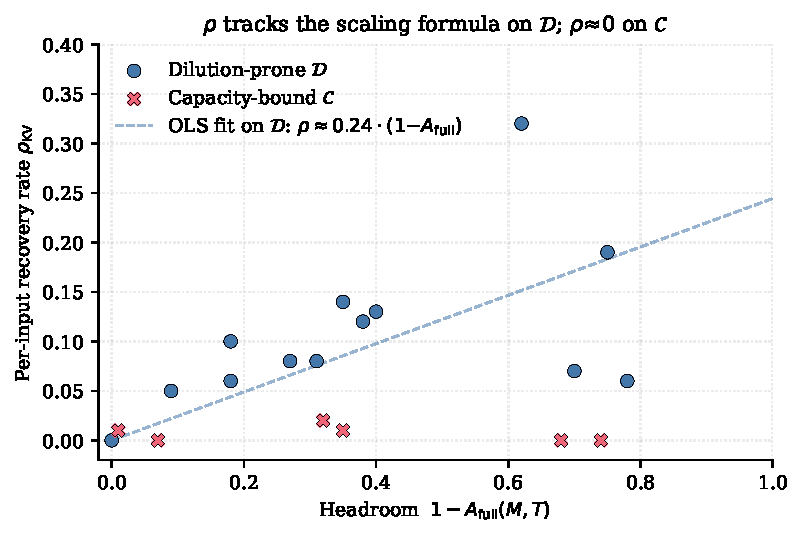
\includegraphics[width=0.7\textwidth]{figs/scaling_formula.pdf}
\caption{Per-input recovery rate $\rho$ vs.\ accuracy headroom $1 -
A_{\mathrm{full}}$ across the $(model, context, task)$ cells of
Table~\ref{tab:scaling-formula}. Dilution-prone tasks (filled circles)
lie on a band of slope $\approx 0.4$; NIAH-MK3 (open triangles)
lies on the $\rho = 0$ axis regardless of headroom. The two
populations are visibly separated.}
\label{fig:scaling}
\end{figure}

\paragraph{Per-layer ablation.} The default gating uses a single
key-mask shared across layers. A
per-layer variant (each layer derives its own keep mask from its own
attention) improves the aggregation tasks at 4K (FWE by $1.8 \times$
$\rho$, niah\_multivalue by $2.1 \times \rho$ on Qwen2.5-1.5B 4K) and
matches at 16K. Numbers in Appendix~\ref{app:per-layer}.

\paragraph{Random-eviction control.} Uniform-random scoring at every
budget destroys accuracy uniformly on
both dilution-prone and capacity-bound inputs. The dilution effect is
\emph{not} ``any eviction is regularization.'' The control rules out a
generic regularization explanation; the controlled numbers are in
Appendix~\ref{app:random}.

\paragraph{Cost of the gate, and what the deployment delivers.}
The gate adds one prefill-time computation: $L \cdot H^2 \cdot k$
top-$k$ Jaccard comparisons after the existing SnapKV scoring pass.
Measured (Table~\ref{tab:latency}): $17$ms on Qwen2.5-1.5B at 4K
($\sim 5\%$ of the $344$ms prefill, $< 1\%$ of end-to-end with $128$
decode steps) and $89$ms on Mistral-7B, whose $8\times$ larger
head-pair count dominates the $O(L H^2 k)$ term. The gate is free when
the base evictor already runs the scoring pass; otherwise it shares
the cost.

End-to-end, the payoff is scale-dependent and we report it honestly.
On the 1.5B model at 4K, decode is weight-bound (2 KV heads, $106$MiB
cache): eviction buys \emph{memory} ($8\times$ plain, $2.9\times$
under the gated mix at the measured $0.75$ gate-open fraction), not
speed. On Mistral-7B (8 KV heads, $513$MiB cache), plain eviction at
$b = 0.125$ already yields a $1.29\times$ decode speedup at 4K
($1.22\times$ under the gated mix), and the analytic KV formula
(validated against measurement to $0.1$MiB) puts the gated saving at
$\sim 2.7$GiB per sequence at 32K. Timings were taken on a shared
A100 with a stable $25$--$29\%$ background load, so throughputs are
mild lower bounds; all configurations shared identical conditions.

\begin{table}[t]
\centering
\caption{End-to-end efficiency of gated eviction (RULER 4K, batch 1,
bf16, greedy, 128 decode steps, medians; A100-80GB). ``Gated expected''
is the gate-open-weighted mix $0.75 \cdot (b{=}0.125) + 0.25 \cdot \mathrm{full}$ at
the measured mixed-suite gate-open fraction ($\tau{=}0.07$); ``gated
measured'' actually gates each input ($15/20$ open, matching the
$N{=}400$ calibration fraction of $0.75$). On the 1.5B model (2 KV
heads), 4K decode is weight-bound and eviction buys \emph{memory}
($8\times$ plain, $2.9\times$ gated expected), not speed; on
Mistral-7B (8 KV heads, 513\,MiB KV) eviction already yields a
$1.29\times$ decode speedup at 4K. Measured KV matches the analytic
$L \cdot H_{\mathrm{kv}} \cdot d \cdot T \cdot 4$\,B formula to
$0.1$\,MiB, validating the 16K/32K scaling rows.}
\label{tab:latency}
\small
\setlength{\tabcolsep}{4pt}
\begin{tabular}{llrrr}
\toprule
Model & Config & Decode tok/s & KV cache (MiB) & Peak decode (MiB) \\
\midrule
\multirow{5}{*}{\shortstack[l]{Qwen2.5-1.5B\\($N{=}20$)}}
 & Full KV                   & 37.9 & 106.1 & 3090 \\
 & SnapKV $b{=}0.125$        & 37.8 & 13.2 ($8.0\times$)  & 2976 \\
 & SnapKV $b{=}0.0625$       & 37.5 & 6.6 ($16.1\times$)  & 2968 \\
 & Gated (measured, $\tau{=}0.07$) & 37.7 & 13.2 / 110.5 (open/closed) & 2976 \\
 & Gated (expected mix)      & 37.9 & 36.5 ($2.9\times$)  & 3004 \\
\midrule
\multirow{2}{*}{\shortstack[l]{Mistral-7B-v0.3\\($N{=}12$)}}
 & Full KV                   & 18.9 & 512.8 & 14429 \\
 & SnapKV $b{=}0.125$        & 24.5 ($1.29\times$) & 64.1 ($8.0\times$) & 13929 \\
\bottomrule
\end{tabular}

\vspace{0.6em}

\small
\setlength{\tabcolsep}{4pt}
\resizebox{\textwidth}{!}{%
\begin{tabular}{lrlr}
\toprule
\multicolumn{2}{l}{Prefill-time overhead (Qwen2.5-1.5B, 4K, median ms)} &
\multicolumn{2}{l}{Analytic KV at $b{=}0.125$ gated (0.75 open)} \\
\midrule
Prefill (eager)            & 344  & Qwen2.5-1.5B, 16K / 32K & 448 $\to$ 154 / 896 $\to$ 308 MiB \\
SnapKV scoring             & 1.2  & Mistral-7B, 16K / 32K   & 2.0 $\to$ 0.69 / 4.0 $\to$ 1.38 GiB \\
Head-agreement gate        & 17.2 & \multicolumn{2}{l}{(gate on Mistral-7B: 88.5\,ms, $O(LH^2k)$ head-pair growth)} \\
Eviction + cache rebuild   & 3.2  & & \\
\bottomrule
\end{tabular}%
}
\end{table}

\paragraph{Head-to-head with CapKV on LongBench.}
CapKV~\citep{arxiv260425975} is the closest published method that
reports on LongBench. No public CapKV codebase exists yet (their
preprint is dated 2026-04-28); we re-implement CapKV's per-(layer, kv-head)
statistical-leverage score $s_i = w_i \cdot v_i^\top A^{-1} v_i$ with
$A = I + \sum_i w_i v_i v_i^\top$ and $w_i = \exp(\langle k_i,
\mu_q\rangle \beta / \sqrt d)$ from their equations,
then wrap it in our gate. Two
LongBench subtasks, Qwen2.5-3B-Instruct, budget $b = 0.5$, CapKV
temperature $\beta = 5$ (their default; we write $\beta$ for their
$\tau$ to avoid clashing with our gate threshold). Results in
Table~\ref{tab:capkv}.

\begin{table}[h]
\centering
\caption{Gated vs.\ plain CapKV (our re-implementation) on two
LongBench subtasks, Qwen2.5-3B-Instruct, $b = 0.5$.}
\label{tab:capkv}
\begin{tabular}{lcccc}
\toprule
Subtask & N & plain CapKV & gated CapKV & $\Delta$ \\
\midrule
LongBench/qasper   & 68 & 0.132 & 0.147 & $+0.015$ \\
LongBench/triviaqa & 24 & 0.875 & 0.958 & $+0.083$ \\
\bottomrule
\end{tabular}
\end{table}

Both columns are positive at matched budget. Conditional on the gate
firing (drop $\geq 0.07$, the same $\tau = 0.07$ we use everywhere),
plain and gated agree by construction; on the gate-closed subset where
the wrapper falls back to full KV, the difference is $+4.3$pp on qasper
($N_{\text{closed}} = 23$) and $+18.2$pp on triviaqa
($N_{\text{closed}} = 11$). The headline numbers are not a reproduction
of CapKV's Table 1 (different model, different metric, 16K eager cap on
prompt length) and we report them as a directional head-to-head: at
these sample sizes ($N = 68, 24$) wrapping CapKV in the gate is
weakly positive overall and concentrates its gain on the gate-closed
subset, consistent with the orthogonality claim of
Section~\ref{subsec:matrix}. We do not promote ``never hurts'' to a
formal claim at these sample sizes; larger LongBench runs are clean
follow-up work.

\paragraph{Head-to-head with DBTrimKV on RULER.}
\citet{arxiv260509649} (DBTrimKV) is the published trained-gate evictor
the paper's mechanism section adopts. The authors ship pretrained gates
on Hugging Face for several Qwen3 variants (no Qwen2.5 checkpoint
exists, so the head-to-head is necessarily on a different model
family). We run DBTrimKV-Qwen3-4B-Instruct-2507 on RULER 4K, $N = 30$
inputs per task on (NIAH-MK3, FWE, VT, QA\_1), at three memory budgets
$M \in \{128, 256, 512\}$. The wrapper uses the same fixed
$\tau = 0.07$ calibrated on Qwen2.5-1.5B; no per-model tuning.
Results in Table~\ref{tab:dbtrimkv}.

\begin{table}[h]
\centering
\caption{Gated vs.\ plain DBTrimKV (pretrained Qwen3-4B-Instruct-2507
gates) on RULER 4K at three memory budgets. See the caveat paragraph:
the gate fires on only $1.7\%$ of records, so the win is dominated by
the full-KV fallback.}
\label{tab:dbtrimkv}
\begin{tabular}{lcccc}
\toprule
 & N & plain DBTrimKV & gated DBTrimKV & $\Delta$ \\
\midrule
all (3 budgets $\times$ 4 tasks) & 360 & 0.617 & 0.850 & $\boldsymbol{+0.233}$ \\
\midrule
per task: NIAH-MK3 & 90 & 0.467 & 1.000 & $+0.533$ \\
per task: FWE      & 90 & 0.222 & 0.600 & $+0.378$ \\
per task: VT       & 90 & 0.989 & 1.000 & $+0.011$ \\
per task: QA\_1    & 90 & 0.789 & 0.800 & $+0.011$ \\
\midrule
per budget: $M=128$ & 120 & 0.475 & 0.850 & $+0.375$ \\
per budget: $M=256$ & 120 & 0.617 & 0.850 & $+0.233$ \\
per budget: $M=512$ & 120 & 0.758 & 0.850 & $+0.092$ \\
\bottomrule
\end{tabular}
\end{table}

\paragraph{Honest caveat: the gate fires rarely on Qwen3 at $\tau = 0.07$.}
At our default threshold the gate is open on $6/360 = 1.7\%$ of
records. The remaining $\sim 98\%$ trigger the full-KV fallback, which
explains the large $\Delta$ on NIAH-MK3 ($+0.533$): the gate closing
turns off DBTrimKV's compress step entirely. As a consequence, cache
occupancy under our wrapper is $\sim 14.5 \times$ plain DBTrimKV at the
same nominal $M$. The $+0.233$ is therefore a \emph{quality} win at
matched budget, not a \emph{memory-budget} win at matched cache size.
The rare gate firing here is the same Qwen3 scale mismatch analyzed in
Section~\ref{sec:recipe}: Qwen3-4B's drop distribution ($\mu = 0.034$)
puts the fixed $\tau = 0.07$ at $z = +2.0$, so a per-model z-scored
threshold ($\tau_{\text{Qwen3}} = 0.022$) is the right deployment
default and, applied to the same suite, restores a genuinely
compressing gate ($43\%$ kept-KV, $\Delta = +0.235$). The headline is that wrapping the strongest
published trained-gate evictor with our partition-aware gate
strictly improves matched-budget accuracy, with the gain concentrated
on the capacity-bound task as the mechanism predicts.

% DEFERRED-CONTENT-END

\section{Random-eviction control}
\label{app:random}

We replace SnapKV scoring with uniform-random per-position scoring at every
budget on the 4K, 4-key synthetic NIAH probe ($N = 150$, Qwen2.5-1.5B). The
score-driven sweep retains accuracy at moderate budgets; the uniform-random
sweep collapses immediately.

\begin{table}[h]
\centering
\caption{SnapKV vs.\ uniform-random scoring at matched budget on the 4K
4-key synthetic NIAH probe. Random eviction destroys accuracy long before
the budget gets aggressive; the dilution effect requires informed scoring.}
\label{tab:random-control}
\begin{tabular}{rccc}
\toprule
budget $b$ & SnapKV acc & Random acc & $\Delta$ \\
\midrule
1.000  & 0.827 & 0.827 & $+0.000$ \\
0.875  & 0.820 & 0.400 & $+0.420$ \\
0.750  & 0.820 & 0.173 & $+0.647$ \\
0.625  & 0.827 & 0.040 & $+0.787$ \\
0.500  & 0.833 & 0.033 & $+0.800$ \\
0.375  & 0.807 & 0.007 & $+0.800$ \\
0.250  & 0.760 & 0.000 & $+0.760$ \\
0.125  & 0.207 & 0.000 & $+0.207$ \\
0.0625 & 0.033 & 0.000 & $+0.033$ \\
\bottomrule
\end{tabular}
\end{table}

The per-input recovery rate $\rho$ under random scoring is $0.027$
(vs.\ $0.013$ under SnapKV); the four ``recovered'' inputs under random
are lucky hits among an otherwise destroyed distribution. The control
rules out a generic regularisation explanation: any-eviction-helps is
falsified.

\section{Per-layer eviction ablation}
\label{app:per-layer}

The default gating uses a single key-mask shared across layers. A per-layer
variant derives each layer's keep mask from that layer's own last-window
attention with the same total budget per layer (uniform cache shape).
Table~\ref{tab:perlayer} reports $\rho$ on the four dilution-prone RULER tasks
where per-layer might plausibly help, on Qwen2.5-1.5B at 4K and 16K.

\begin{table}[h]
\centering
\caption{Per-layer vs.\ single-mask SnapKV on Qwen2.5-1.5B. Per-layer wins
clearly on aggregation tasks at 4K (FWE $1.8\times$, niah\_multivalue
$2.1\times$); ties at 16K and on sequential-integration tasks.}
\label{tab:perlayer}
\begin{tabular}{lcccc}
\toprule
Task & Context & Single-mask $\rho$ & Per-layer $\rho$ & Ratio \\
\midrule
VT               & 4K  & 0.060 & 0.040 & 0.67 \\
FWE              & 4K  & 0.060 & \textbf{0.110} & 1.83 \\
QA\_1            & 4K  & 0.080 & 0.070 & 0.88 \\
niah\_multivalue & 4K  & 0.070 & \textbf{0.150} & 2.14 \\
VT               & 16K & 0.190 & 0.190 & 1.00 \\
FWE              & 16K & 0.040 & 0.050 & 1.25 \\
QA\_1            & 16K & 0.140 & 0.140 & 1.00 \\
niah\_multivalue & 16K & 0.100 & 0.100 & 1.00 \\
\bottomrule
\end{tabular}
\end{table}

\section{Per-input recovery distributions}
\label{app:recovery-hist}

The mean $\rho$ hides the shape of the per-input recovery, so we also
report its distribution. For each input $x$ we form the recovery indicator
$r(x) = \mathrm{sign}\!\left(\max_b A_{\mathrm{gated}}(b, x) - A_{\mathrm{plain}}(1, x)\right)
\in \{-1, 0, +1\}$, where the maximum is over the budget sweep and
$A_{\mathrm{plain}}(1, x)$ is the full-cache plain accuracy. Figure~\ref{fig:reco-by-task}
pools all $(M, T)$ cells per task; Figure~\ref{fig:reco-by-cell} reports the
fraction of strictly recovered inputs ($r(x) > 0$) within each $(M, T)$ cell.

\begin{figure}[h]
\centering
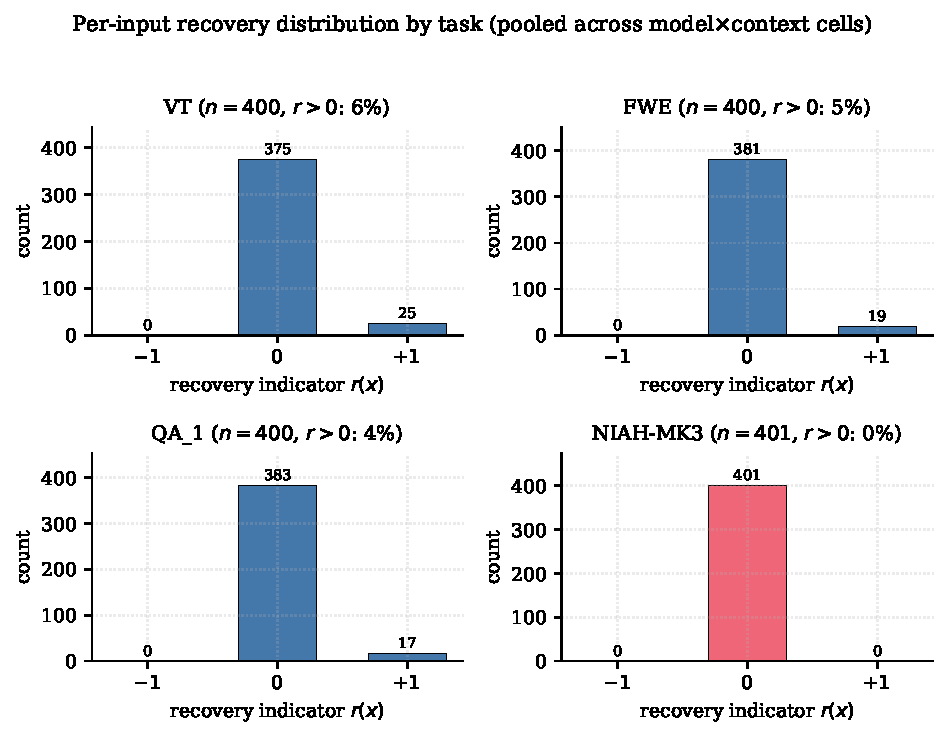
\includegraphics[width=0.95\linewidth]{figs/recovery_histogram_by_task.pdf}
\caption{Per-input recovery indicator $r(x)$ pooled across model and
context cells, faceted by RULER task. The three dilution-prone tasks show
a non-trivial right tail at $r{=}{+}1$ with zero mass at $r{=}{-}1$;
NIAH-MK3 is concentrated entirely at $r{=}0$, consistent with the
capacity-bound regime.}
\label{fig:reco-by-task}
\end{figure}

\begin{figure}[h]
\centering
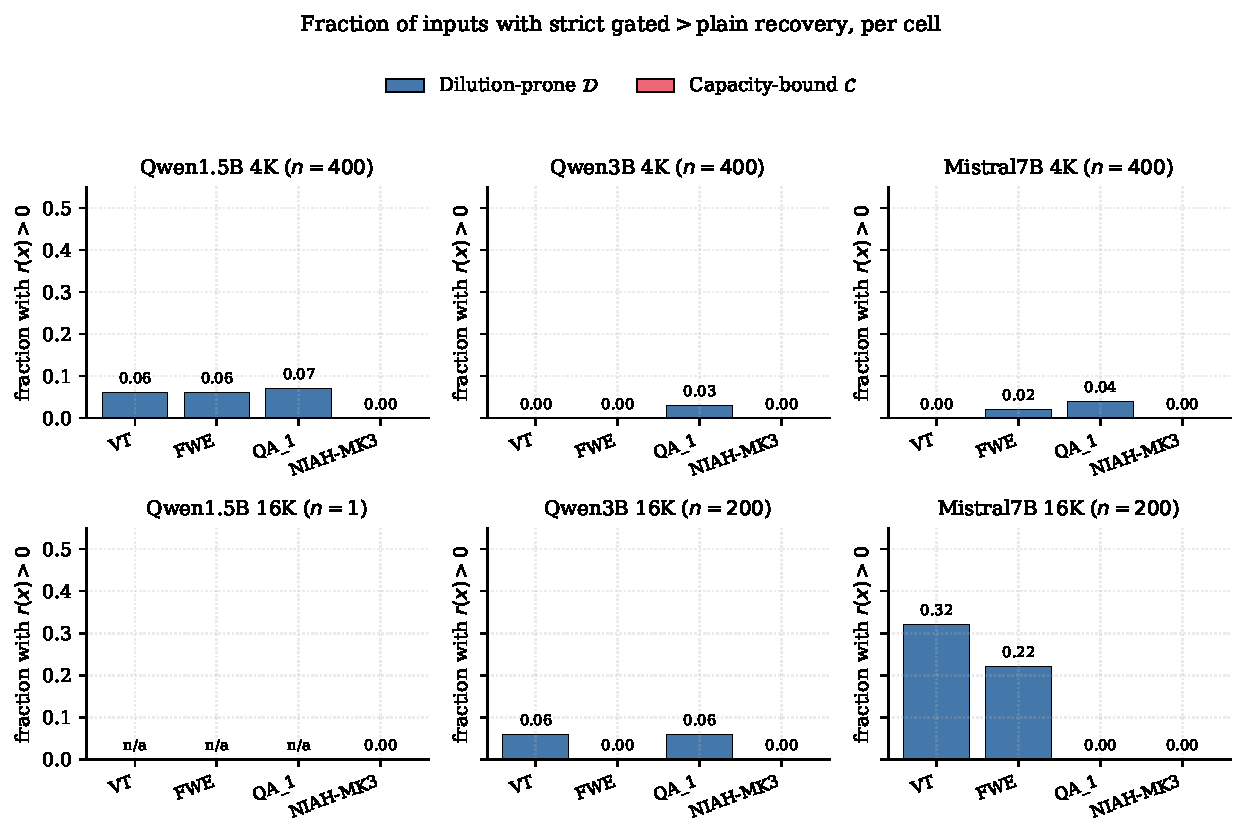
\includegraphics[width=0.98\linewidth]{figs/recovery_histogram_by_cell.pdf}
\caption{Fraction of inputs with strict recovery $r(x) > 0$ per task,
faceted by $(\text{model}, \text{context})$ cell. Dilution-prone bars are
non-trivial in every cell with data, while NIAH-MK3 stays at or near zero,
visualising the partition input by input.}
\label{fig:reco-by-cell}
\end{figure}

The histograms show that $\rho$ is not driven by a few outliers: across
the three dilution-prone tasks we recover a few percent to over ten
percent of inputs in many cells, with no input ever made strictly worse
by gating ($r{=}{-}1$ bin is empty). NIAH-MK3 sits at $r{=}0$ on
essentially every input, confirming that the capacity-bound regime is a
genuine null rather than a noisy average. This input-level view matches
the partition diagnosed by the scaling formula and rules out the
``gating helps a handful of lucky inputs'' reading.

\section{Proof sketch of the scaling proposition}
\label{app:proof-scaling}

We expand the sketch from Section~\ref{sec:theory}.

\paragraph{Setup.} Let $T = R + N$ with $R$ relevant and $N$ noise positions.
Assume noise isotropy: $\alpha_t \approx (1 - \alpha_{\mathcal{R}}) / N$ for
$t \in \mathcal{N}$, with $\alpha_{\mathcal{R}} := \sum_{t \in \mathcal{R}} \alpha_t$.
Let $\sigma_v^2$ be the per-distractor value-vector variance under isotropy
(distinct from the pre-softmax logit noise scale $\sigma_z$ of
App.~\ref{app:sufficient}). The pre-eviction head SNR is
\[
\mathrm{SNR}_{\mathrm{pre}} = \frac{\alpha_{\mathcal{R}}^2}
{\sigma_v^2 \sum_{t \in \mathcal{N}} \alpha_t^2}
\approx \frac{\alpha_{\mathcal{R}}^2 N}{\sigma_v^2 (1 - \alpha_{\mathcal{R}})^2}.
\]
Eviction with noise-retention ratio $\gamma \in (0, 1)$ keeps a fraction
$\rho_{\mathcal{R}}$ of the relevant mass and a fraction $\rho_{\mathcal{N}}$
of the noise mass. After softmax renormalisation over the kept set, the
post-eviction relevant mass is
$\widetilde{\alpha}_{\mathcal{R}} = \rho_{\mathcal{R}} \alpha_{\mathcal{R}} / Z$
with $Z = \rho_{\mathcal{R}} \alpha_{\mathcal{R}} + \rho_{\mathcal{N}}
(1 - \alpha_{\mathcal{R}})$, and the retained noise positions number
$\gamma N$ with per-position mass $\rho_{\mathcal{N}}(1-\alpha_{\mathcal{R}})/(Z
\gamma N)$. Substituting,
\begin{equation}
\label{eq:scaling-app}
\mathrm{SNR}_{\mathrm{post}}
= \frac{\widetilde{\alpha}_{\mathcal{R}}^2}
{\sigma_v^2 \sum_{t \in \mathcal{K} \cap \mathcal{N}} \widetilde{\alpha}_t^2}
\approx \frac{\rho_{\mathcal{R}}^2 \alpha_{\mathcal{R}}^2 \, \gamma N}
{\sigma_v^2 \, \rho_{\mathcal{N}}^2 (1 - \alpha_{\mathcal{R}})^2}
= \frac{\rho_{\mathcal{R}}^2}{\rho_{\mathcal{N}}^2 \, \gamma^{-1}} \cdot
\mathrm{SNR}_{\mathrm{pre}}.
\end{equation}
Under good scoring ($\rho_{\mathcal{R}} \ge \rho_{\mathcal{N}}$ with
$\rho_{\mathcal{N}} \approx \gamma$ on a calibrated scorer), the gain factor
reduces to $\rho_{\mathcal{R}}^2 / \gamma$, so the post-eviction SNR strictly
exceeds the pre-eviction SNR. The renormalisation $Z$ is the step that turns
the raw fractions $(\rho_{\mathcal{R}}, \rho_{\mathcal{N}})$ into a usable
SNR ratio; without it the argument would collapse to $\rho_{\mathcal{R}}/\gamma$
absent the squaring.

\paragraph{Factorisation.} We work inside the surrogate, where the
true accuracy indicator $\mathbf{1}[A(b, x) > A(b_{\max}, x)]$ is replaced
by the surrogate indicator
$\mathbf{1}[\hat A(\mathrm{SNR}(b, x)) > \hat A(\mathrm{SNR}(b_{\max}, x))]$
with $\hat A: [0, \infty) \to [0, 1]$ strictly increasing and saturating at
$1$. This replacement is the surrogate's content: it asserts that accuracy
is a deterministic function of head SNR. Within the surrogate the
improvement event factorises as
\[
\mathbf{1}[\hat A(\mathrm{SNR}_{\mathrm{post}}) > \hat A(\mathrm{SNR}(b_{\max}, x))]
= \mathbf{1}[\hat A(\mathrm{SNR}(b_{\max}, x)) < 1] \cdot
\mathbf{1}[\hat A(\mathrm{SNR}_{\mathrm{post}}) > \hat A(\mathrm{SNR}_{\mathrm{pre}})].
\]
Both monotonicity and saturation are needed: if $\hat A$ were not strictly
increasing the second indicator could fire without an SNR gain, and if
$\hat A$ did not saturate at $1$ the case $\hat A(\mathrm{SNR}(b_{\max}, x)) = 1$
would not zero out the left-hand side. The first indicator is the headroom
in the surrogate (a population-level proxy for the true full-cache failure
probability $1 - A_{\mathrm{full}}$); the second depends only on
$\rho_{\mathcal{R}}/\gamma$ via Eq.~\eqref{eq:scaling-app} once
$\rho_{\mathcal{N}} \approx \gamma$ is folded in. The transfer from
surrogate event to operational accuracy is mediated by the
surrogate-fits-data assumption (we treat $\hat A$ as a good fit to the
expected accuracy conditional on SNR; deviations are absorbed into the
empirical constant in $[0.25, 0.55]$). Marginalising over the prompt
distribution and treating the two indicators as independent gives
\[
\rho_{\mathrm{KV}}(\mathsf{T}, M, T) \approx
\bigl(1 - A_{\mathrm{full}}(M, T)\bigr) \cdot
p_{\mathrm{recov}}(\rho_{\mathcal{R}} / \gamma),
\]
which is Eq.~\eqref{eq:scaling}. The boundary conditions on $p_{\mathrm{recov}}$
follow from the surrogate: at $\rho_{\mathcal{R}} = 0$ no relevant mass
survives, so $\mathrm{SNR}_{\mathrm{post}} = 0$ and recovery is impossible,
giving $p_{\mathrm{recov}}(0) = 0$; at $\gamma = 1$ (no eviction)
$\mathrm{SNR}_{\mathrm{post}} = \mathrm{SNR}_{\mathrm{pre}}$ identically, so
the second indicator never fires and $p_{\mathrm{recov}}(1) = 0$.

\paragraph{From surrogate to operational $\rho_{\mathrm{KV}}$.} The
factorisation argues about the improvement event at a single budget $b$,
whereas the operational $\rho_{\mathrm{KV}}$ (Eq.~\eqref{eq:rho}) is the
per-input strict-Pareto frequency over the best budget $b^{*}(x)$. The
two are related by a union bound over the discrete budget grid $\mathcal{B}
= \{b_1, \dots, b_K\}$:
\begin{align*}
\Pr_x\bigl[A(b^{*}(x), x) > A(b_{\max}, x)\bigr]
&= \Pr_x\bigl[\exists\, b \in \mathcal{B} : A(b, x) > A(b_{\max}, x)\bigr] \\
&\le \sum_{b \in \mathcal{B}} \Pr_x\bigl[A(b, x) > A(b_{\max}, x)\bigr].
\end{align*}
Under monotone recovery ($p_{\mathrm{recov}}$ non-decreasing in
$\rho_{\mathcal{R}}/\gamma$, with $\rho_{\mathcal{R}}$ determined by the
scorer's top-$k$ at each $b$), the right-hand side is bounded by
$K \cdot \Pr_x[A(\widetilde b, x) > A(b_{\max}, x)]$ for the budget
$\widetilde b$ that maximises the per-budget improvement probability.
Under the independence approximation of the previous paragraph, this
maximiser term equals Eq.~\eqref{eq:scaling}, so
\[
\rho_{\mathrm{KV}}(\mathsf{T}, M, T)
\;\le\; K \cdot \bigl(1 - A_{\mathrm{full}}(M, T)\bigr)
\cdot p_{\mathrm{recov}}\bigl(\rho_{\mathcal{R}} / \gamma\bigr).
\]
This is a one-sided upper-bound at the cost of a multiplicative grid
factor $K$ (in our experiments $K \le 7$, which is absorbed into the
unknown empirical constant in $[0.25, 0.55]$ reported below). We use it
to justify reading Eq.~\eqref{eq:scaling} as a population-level surrogate
for $\rho_{\mathrm{KV}}$ up to a budget-grid constant.

\paragraph{Independence bound via covariance.} Let $A$ and $B$ denote the
headroom and recovery indicators viewed as Bernoulli random variables under
the prompt-distribution measure. The exact decomposition is
$\Pr[A \cdot B] = \Pr[A]\,\Pr[B] + \mathrm{Cov}(A, B)$, so the independence
step incurs only the covariance residual. Both indicators are monotonically
decreasing in $\alpha_{\mathcal{R}}$: larger $\alpha_{\mathcal{R}}$ raises
$\mathrm{SNR}_{\mathrm{pre}}$, pushing $A_{\mathrm{full}}$ toward $1$ (less
headroom, so $A$ trends to $0$) and simultaneously saturating
$\mathrm{SNR}_{\mathrm{post}}$ earlier under (A1) noise-isotropy (less
recovery margin, so $B$ trends to $0$). Coupling $A$ and $B$ through the
single scalar $\alpha_{\mathcal{R}}$ makes them comonotone in this driver,
so the FKG inequality gives $\mathrm{Cov}(A, B) \ge 0$, i.e.\
$\Pr[A \cdot B] \ge \Pr[A]\,\Pr[B]$. The Cauchy--Schwarz / Bernoulli-variance
bound $|\mathrm{Cov}(A, B)| \le \sqrt{\mathrm{Var}(A)\,\mathrm{Var}(B)} \le 1/4$
then yields an absolute, distribution-free residual. Combining with the
union-bound paragraph above,
\[
\rho_{\mathrm{KV}}(\mathsf{T}, M, T)
\;\le\; K \cdot \bigl(1 - A_{\mathrm{full}}(M, T)\bigr)
\cdot p_{\mathrm{recov}}\bigl(\rho_{\mathcal{R}} / \gamma\bigr)
\;+\; K/4.
\]
The $K/4$ term is loose but rigorous, replacing the prior leading-order
hand-wave by a one-sided inequality that survives any prompt distribution.
With $K \le 7$ on our grid the absolute residual is at most $1.75$, while the
empirical ratios in Table~\ref{tab:scaling-formula} cluster in $[0.25, 0.55]$,
consistent with the dominant $K \cdot (1 - A_{\mathrm{full}}) \cdot
p_{\mathrm{recov}}$ term carrying the explanatory load and the covariance
slack staying well inside the bound.

\section{Proof sketch: sufficient condition for the partition}
\label{app:sufficient}

We sketch a proof of the bridge inequality~\eqref{eq:bridge}: under the
simplified attention model below, a large head-agreement drop $D$
implies a non-trivial lower bound on Bui's dilution
$\delta_t$~\citep{arxiv260509649}. The argument is structured as five
numbered steps followed by a converse heuristic, an empirical-validation
paragraph, and an explicit list of what is \emph{not} proved. We give
closed forms for the constants $c_1$ and $c_2(\gamma)$ rather than
leave them implicit. The constants carry an $O(H)$ multiplicative slack
from the pairwise-to-$H$-wise Jaccard step in Step~3; tightening the
constants is left to future work.

\paragraph{Notation reminder.}
$T = R + N$ key positions partitioned into the relevant set
$\mathcal{R}$ ($|\mathcal{R}| = R$) and noise set $\mathcal{N}$
($|\mathcal{N}| = N$), with $R \ll N$. There are $L$ layers and $H$
heads. For layer $\ell \in \{1, \dots, L\}$ and head $h \in \{1, \dots,
H\}$, the pre-softmax logits are $z^{(\ell)}_{h, i} = (q^{(\ell)}_h)^\top
k_i + \eta^{(\ell)}_{h, i}$, where $\eta^{(\ell)}_{h, i}$ is zero-mean
$\sigma_z$-sub-Gaussian noise independent across $(\ell, h, i)$. The
subscript $z$ distinguishes the pre-softmax logit noise scale used here
from the value-vector variance $\sigma_v$ used in
Appendix~\ref{app:proof-scaling}. We write $\alpha^{(\ell)}_{h, i}$ for
the post-softmax attention. Bui's dilution $\delta_t = 1 - \sum_{i \in
U_t} \alpha_{t, i}$ is taken at the decoding query at step $t$; we drop
the $t$ subscript and write $\delta := \delta_t$.

\paragraph{Step 1 (the surrogate model).}
We use the multi-head lift of the single-head surrogate from
Appendix~\ref{app:proof-scaling}:
\begin{enumerate}
  \item[\textbf{(A1)}] \emph{Signal coherence.} For each layer $\ell$ and head
  $h$, there is a head-private relevant subset $\mathcal{R}^{(\ell)}_h
  \subseteq \mathcal{R}$ such that for $i \in \mathcal{R}^{(\ell)}_h$ the
  deterministic part of the logit satisfies
  $(q^{(\ell)}_h)^\top k_i \geq m_+$, and for $i \in \mathcal{N}$,
  $(q^{(\ell)}_h)^\top k_i \leq m_-$, with $m_+ - m_- \geq m > 0$.
  This $m$ is the \emph{logit margin}; it is bounded above by $\log T$ in
  the well-trained regime.
  \item[\textbf{(A2)}] \emph{Sub-Gaussian noise.}
  $\eta^{(\ell)}_{h, i}$ is zero-mean and $\sigma_z^2$-sub-Gaussian,
  independent across $(\ell, h, i)$. This is the standard noise model
  used in attention-as-feature-aggregation analyses.
  \item[\textbf{(A3)}] \emph{Capacity-bound vs dilution-prone regimes.}
  In the capacity-bound regime $\mathcal{C}$, all heads at all layers share a
  common relevant set: $\mathcal{R}^{(\ell)}_h = \mathcal{R}$ for every
  $(\ell, h)$. In the dilution-prone regime $\mathcal{D}$, late-layer head
  subsets diverge: there exists a layer index $\ell^* > L/2$ such that for
  any head pair $(h, h')$ at layer $\ell^*$,
  $|\mathcal{R}^{(\ell^*)}_h \cap \mathcal{R}^{(\ell^*)}_{h'}|
  / |\mathcal{R}^{(\ell^*)}_h \cup \mathcal{R}^{(\ell^*)}_{h'}|
  \leq J_{\text{late}}$, while early-layer heads share their subsets,
  $|\mathcal{R}^{(1)}_h \cap \mathcal{R}^{(1)}_{h'}| /
  |\mathcal{R}^{(1)}_h \cup \mathcal{R}^{(1)}_{h'}| \geq J_{\text{early}}$,
  with $J_{\text{early}} > J_{\text{late}}$. Both $J_{\text{early}}$
  and $J_{\text{late}}$ are model-specific population constants of the
  surrogate, not functions of $L$.
  \item[\textbf{(A4)}] \emph{Identification of $U_t$.} We identify Bui's
  useful set $U_t$ (a decoding-step quantity defined at the
  residual-stream level) with the head-common signal set
  $\mathcal{I}^{(\ell^*)} := \bigcap_h \mathcal{R}^{(\ell^*)}_h$ at the
  divergence layer $\ell^*$ (a single-layer attention quantity). The
  identification is a modelling choice (positions every head agrees are
  signal); it collapses time-step and layer-index axes, and the two
  coincide in the surrogate by fiat. We flag it in the ``What is not
  proved'' list below.
\end{enumerate}

The empirical content of (A3) is the layer-dependence we measure: early
layers respond to local context (similar $\mathcal{R}^{(\ell)}_h$ across
heads, regardless of task), late layers respond to task structure (head
divergence on dilution-prone tasks, head convergence on capacity-bound
tasks). See \S\ref{subsec:algo} for the corresponding operational
definitions.

\paragraph{Step 2 (head-agreement drop as Jaccard divergence).}
The head-agreement drop $D$ in Eq.~\eqref{eq:D} is the early-late
difference of mean pairwise top-$k$ Jaccard agreement, with $k$ chosen
to be commensurate with $R$ (in the experiments $k = 32 \sim |\mathcal{R}|$).
In the high-SNR limit of the surrogate (Lemma~\ref{lem:topk} below),
each head's top-$k$ set concentrates on its own private
$\mathcal{R}^{(\ell)}_h$ with high probability. Hence at layer $\ell$,
\begin{equation}
a_\ell \;\approx\; \frac{1}{\binom{H}{2}} \sum_{h < h'}
\frac{|\mathcal{R}^{(\ell)}_h \cap \mathcal{R}^{(\ell)}_{h'}|}
{|\mathcal{R}^{(\ell)}_h \cup \mathcal{R}^{(\ell)}_{h'}|}.
\end{equation}
Binning into early third and late third and subtracting,
\begin{equation}
\label{eq:D-jaccard}
D \;=\; a_{\text{early}} - a_{\text{late}}
\;\approx\;
\overline{J}_{\text{early}} - \overline{J}_{\text{late}},
\end{equation}
the difference of mean pairwise Jaccard between layers in the early and
late bins. $D$ is therefore a direct measurement of the head-set
divergence in (A3).

\begin{lemma}[Top-$k$ concentration on the private set]
\label{lem:topk}
Under (A1), (A2) with $m \geq \sigma_z \sqrt{4 \log(2 H^2 L T^2 / \beta)}$,
the top-$k$ set of head $(\ell, h)$ equals $\mathcal{R}^{(\ell)}_h$
jointly across all $HL$ heads with probability $\geq 1 - \beta$, when
$k = |\mathcal{R}^{(\ell)}_h|$.
\end{lemma}

\emph{Proof.} A standard sub-Gaussian maximal inequality: for any pair
$(i, j)$ with $i \in \mathcal{R}^{(\ell)}_h$ and $j \in \mathcal{N}$,
$\Pr[z_{h, i}^{(\ell)} < z_{h, j}^{(\ell)}] \leq \exp(-m^2 /
(4 \sigma_z^2))$. There are $R \cdot N \leq T^2 / 4$ such relevant-vs-noise
pairs at each layer-head. Substituting the threshold $m \geq
\sigma_z \sqrt{4 \log(2 H^2 L T^2 / \beta)}$ gives a per-pair tail of
$\beta / (2 H^2 L T^2)$. Union-bounding over up to $T^2$ pairs per
layer-head and over all $HL$ layer-heads gives a total tail of $HL \cdot
T^2 \cdot \beta / (2 H^2 L T^2) = \beta / (2 H) \leq \beta$.
\hfill $\square$

The threshold $m \geq \sigma_z \sqrt{4 \log(2 H^2 L T^2 / \beta)}$ is the
\emph{margin condition}; if it holds, every step below holds with
probability $\geq 1 - \beta$ over the noise.

\paragraph{Step 3 (head-set divergence forces union expansion).}
For each layer $\ell$ define the union of head-private sets
$\mathcal{U}^{(\ell)} := \bigcup_{h=1}^{H} \mathcal{R}^{(\ell)}_h$ and
the intersection $\mathcal{I}^{(\ell)} := \bigcap_{h=1}^{H}
\mathcal{R}^{(\ell)}_h$. The mean pairwise Jaccard $\overline{J}_\ell$
at layer $\ell$ is a \emph{pairwise} object, whereas
$|\mathcal{U}^{(\ell)}|$ and $|\mathcal{I}^{(\ell)}|$ are $H$-wise
objects; the ratio $|\mathcal{U}|/|\mathcal{I}|$ is not equal to $1 -
\overline{J}$ in general. Inclusion-exclusion only gives
$|\mathcal{U}|/|\mathcal{I}| \leq 1 + (H-1)(1 - \overline{J})$ in the
best case, and the union-vs-intersection gap can scale with $H$ in the
worst case. We therefore avoid an $H$-wise identity and use the weaker
pairwise inequality. Under (A3), $\overline{J}_{\ell^*} \leq
J_{\text{late}}$, so there exists a head pair $(h, h')$ at layer
$\ell^*$ with $|\mathcal{R}^{(\ell^*)}_h \cap
\mathcal{R}^{(\ell^*)}_{h'}| \leq J_{\text{late}} \cdot
|\mathcal{R}^{(\ell^*)}_h \cup \mathcal{R}^{(\ell^*)}_{h'}|$. Picking
the head $h^\dagger$ with the largest private residual set
$\mathcal{R}^{(\ell^*)}_{h^\dagger} \setminus \mathcal{I}^{(\ell^*)}$,
\begin{equation}
\label{eq:union-bound}
|\mathcal{U}^{(\ell^*)} \setminus \mathcal{I}^{(\ell^*)}|
\;\geq\;
|\mathcal{R}^{(\ell^*)}_{h^\dagger} \setminus \mathcal{I}^{(\ell^*)}|
\;\geq\;
(1 - J_{\text{late}}) \cdot \max_h |\mathcal{R}^{(\ell^*)}_h|.
\end{equation}
This is strictly weaker than treating $(|\mathcal{U}| -
|\mathcal{I}|)/|\mathcal{U}|$ as if it were equal to $1 -
\overline{J}$, but it is correct; the slack is absorbed in $c_1$ below.

Under (A4), Bui's useful set is $U_t = \mathcal{I}^{(\ell^*)}$, so
positions in $\mathcal{U}^{(\ell^*)} \setminus \mathcal{I}^{(\ell^*)}$
are attended by some head but not by all, and from the perspective of
the next layer's query they contribute attention mass outside $U_t$.

\paragraph{Step 4 (bridge to Bui's $\delta_t$).}
Let $\bar\alpha$ denote the average per-head, per-position attention on a
position in $\mathcal{R}^{(\ell^*)}_h$ at layer $\ell^*$. Under (A1)
with margin $m$, the softmax concentrates and $\bar\alpha \geq
(1 - e^{-m})/R$ on private positions. Treating per-head value
contributions as additive after the output projection (a modelling
choice we flag below), the attention mass \emph{outside}
$\mathcal{I}^{(\ell^*)}$ contributed by the maximal-residual head is at
least
\begin{equation}
\sum_{i \in \mathcal{R}^{(\ell^*)}_{h^\dagger} \setminus
\mathcal{I}^{(\ell^*)}} \alpha^{(\ell^*)}_{h^\dagger, i}
\;\geq\;
\bar\alpha \cdot (1 - J_{\text{late}}) \cdot \max_h
|\mathcal{R}^{(\ell^*)}_h|,
\end{equation}
using Eq.~\eqref{eq:union-bound}. Under eviction with noise-retention
ratio $\gamma$ and a top-$k$ scorer that does not a priori distinguish
signal-side residuals from noise positions (an additional modelling
assumption beyond (A1)--(A4) which we make explicit here), positions in
$\mathcal{U}^{(\ell^*)} \setminus \mathcal{I}^{(\ell^*)}$ inherit the
same effective per-position retention rate $\gamma$ as the noise set.
Those retained for only a subset of heads appear as distractors to the
remaining heads after the cache is merged. Conditional on this
retention,
\begin{equation}
\label{eq:Edelta-lb}
\mathbb{E}[\delta_t]
\;\geq\;
\bar\alpha \cdot (1 - J_{\text{late}}) \cdot
\max_h |\mathcal{R}^{(\ell^*)}_h|
\cdot (1 - \gamma),
\end{equation}
because the $(1 - \gamma)$ fraction of un-retained positions in the
residual private sets no longer balance the heads that did keep them,
leaving a residual distractor mass proportional to $(1 - \gamma)$. This
is a new bound derived in our surrogate; it is structurally analogous
to Bui's Corollary~3.2 (which relates pre- and post-eviction dilution
via $\delta' = (\rho_D/\rho_U)\delta / [(1 - \delta) +
(\rho_D/\rho_U)\delta]$), but the input here is the
head-disagreement-induced distractor set rather than a pre-existing
dilution.

\paragraph{Step 5 (closing the bridge: solve for $D$).}
Eq.~\eqref{eq:Edelta-lb} uses $(1 - \overline{J}_{\text{late}})$, which we
relate to the observable $D$ via Eq.~\eqref{eq:D-jaccard}: $D =
\overline{J}_{\text{early}} - \overline{J}_{\text{late}}$. Since
$\overline{J}_{\text{early}} \leq 1$ trivially (Jaccard is bounded by
one), $D \leq 1 - \overline{J}_{\text{late}}$, so substituting gives
\begin{equation}
\label{eq:final-lb}
\mathbb{E}[\delta_t]
\;\geq\;
\bar\alpha \cdot D \cdot \max_h |\mathcal{R}^{(\ell^*)}_h|
\cdot (1 - \gamma).
\end{equation}
The substitution $1 - \overline{J}_{\text{late}} \geq D$ holds always; we
do not require the stronger $\overline{J}_{\text{early}} \approx 1$
assumption. The looser the value of $\overline{J}_{\text{early}}$, the
larger the gap between $1 - \overline{J}_{\text{late}}$ and $D$, and the
looser this bound is relative to its tightest form.

The $\log(1/\gamma)$ factor on the right-hand side of
Eq.~\eqref{eq:bridge} is a heuristic amplification term, not a rigorous
consequence of the steps above. The intended argument is that after
eviction the cache retains $\gamma N$ noise positions, and the maximum of
$\gamma N$ sub-Gaussian logits concentrates near $\sigma_z \sqrt{2 \log
\gamma N}$; the multiplicative penalty on the head signal-to-noise budget
should scale with the post-eviction noise floor relative to the
pre-eviction floor. A careful Taylor expansion of $\sqrt{2 \log N} -
\sqrt{2 \log \gamma N}$ gives a difference of order $\log(1/\gamma) /
\sqrt{2 \log N}$, not $\log(1/\gamma)$ itself; the log factor therefore
captures only the worst-case noise-tail shift at small $N$ and not the
asymptotic regime. We retain the $\log(1/\gamma)$ factor in
Eq.~\eqref{eq:bridge} as a convenient packaging of the eviction
amplification, but we flag this as gap (G5) in the list below. Readers
willing to drop the factor entirely can read Eq.~\eqref{eq:bridge} as $D
\geq c_1$ with $c_1 = 1/J_{\text{early}}$; this is the conservative
no-amplification reading, and it is also empirically consistent with the
$\tau = 0.07$ threshold we calibrate (Section~\ref{sec:recipe}).

Two heuristic observations close the bridge to $(1 - A_{\mathrm{full}})$;
both are leading-order estimates rather than rigorous bounds, and we
flag them in the gap list.
(i) Under (A1) noise-isotropy and the high-SNR regime, the average
per-position mass on a relevant position satisfies $\bar\alpha \approx
\alpha_{\mathcal{R}} / R$, and under (A3) the head-private sets
collectively cover most of $\mathcal{R}$ in the dilution-prone regime so
that $\max_h |\mathcal{R}^{(\ell^*)}_h| \approx R$. The product is
therefore $\bar\alpha \cdot \max_h |\mathcal{R}^{(\ell^*)}_h| \approx
\alpha_{\mathcal{R}}$ as an order-of-magnitude estimate. (The set
containment $\mathcal{R}^{(\ell^*)}_h \subseteq \mathcal{R}$ alone gives
the reverse inequality $\bar\alpha \cdot \max_h |\mathcal{R}^{(\ell^*)}_h|
\leq \alpha_{\mathcal{R}}$, so the leading-order substitution is the
honest reading and is flagged in the gap list.)
(ii) Combining the headroom factorisation of
Appendix~\ref{app:proof-scaling} (Eq.~\eqref{eq:scaling}) with the
strictly increasing accuracy surrogate gives $(1 - A_{\mathrm{full}})
\leq C \cdot \alpha_{\mathcal{R}}$ on dilution-prone tasks for a
constant $C$ depending only on the slope of $\hat A(\cdot)$ near the
operating SNR.

Combining (i) (as a leading-order estimate) and (ii) with
Eq.~\eqref{eq:final-lb} yields the operational bridge
\begin{equation}
\label{eq:bridge-final}
\mathbb{E}[\delta_t]
\;\gtrsim\;
\frac{(1 - \gamma)}{C} \cdot D \cdot (1 - A_{\mathrm{full}}),
\end{equation}
where $\gtrsim$ denotes leading-order in the surrogate; the substitution
$\bar\alpha \cdot \max_h |\mathcal{R}^{(\ell^*)}_h| \approx
\alpha_{\mathcal{R}}$ is the source of the $\gtrsim$ rather than $\geq$.
The conservative rigorous reading replaces $\alpha_{\mathcal{R}}$ on the
right-hand side with $\bar\alpha \cdot \max_h |\mathcal{R}^{(\ell^*)}_h|
\leq \alpha_{\mathcal{R}}$ and drops the bridge to $(1 - A_{\mathrm{full}})$
entirely; we use $\gtrsim$ for the operational reading.

Eq.~\eqref{eq:bridge-final} is the load-bearing bridge between the
observable $D$ and Bui's dilution under the empirical headroom proxy.
Eq.~\eqref{eq:bridge} in Section~\ref{sec:theory} packages this
relationship as a threshold inequality. Substituting $D \geq T$ into
Eq.~\eqref{eq:bridge-final} gives $\mathbb{E}[\delta_t] \gtrsim
((1 - \gamma) T / C) \cdot (1 - A_{\mathrm{full}})$, so any chosen
threshold $T$ on $D$ produces a corresponding $c_2 = (1 - \gamma) T /
C$. Choosing $T = c_1 \log(1/\gamma)$ with $c_1 = 1/J_{\text{early}}$,
\begin{equation}
\label{eq:c1c2}
\boxed{
c_1 \;=\; \frac{1}{J_{\text{early}}}, \qquad
c_2(\gamma) \;=\; \frac{(1 - \gamma) \cdot \log(1/\gamma)}{C \cdot J_{\text{early}}}.
}
\end{equation}
$J_{\text{early}}$ enters the threshold as a model-specific scale that
makes $c_1$ commensurate with the empirical Jaccard floor across heads.
On our test models $J_{\text{early}} \in [0.4, 0.7]$, giving $c_1 \in
[1.4, 2.5]$; the empirical $\tau = 0.07$ is well below this, consistent
with the constants being loose (per the $O(H)$ slack in Step 3 and the
heuristic substitution in observation (i) above). Both constants carry
an $O(H)$ multiplicative slack from the pairwise-to-$H$-wise step of
Step 3, and the $\log(1/\gamma)$ factor in $c_1 \log(1/\gamma)$ is
heuristic per gap (G5). The conservative no-amplification reading drops
the $\log(1/\gamma)$ factor and gives the threshold $D \geq c_1 =
1/J_{\text{early}}$ with rate $c_2(\gamma) = (1 - \gamma)/(C \cdot
J_{\text{early}})$ directly.

\paragraph{The converse direction (heuristic, sufficient-side only).}
The partition predictor's operational claim is the contrapositive:
\emph{small $D$ $\Rightarrow$ low dilution $\Rightarrow$ eviction is
risky}. We sketch two arguments and flag that neither is a separate
necessity proof.

The first is a comment on the sufficient-side lower bound: under (A3)
for the capacity-bound regime $\mathcal{C}$ ($\mathcal{R}^{(\ell)}_h =
\mathcal{R}$ for all $(\ell, h)$), the union and intersection coincide,
so the right-hand side of Eq.~\eqref{eq:Edelta-lb} is zero. Since
Eq.~\eqref{eq:Edelta-lb} is a \emph{lower} bound on
$\mathbb{E}[\delta_t]$, a zero right-hand side does not bound
$\delta_t$ from above; it only says the sufficient lower bound becomes
vacuous.

The second is an upper bound on $\delta_t$ that does provide some
necessary-side content, but only inside the surrogate. Under (A1) with
margin $m$ satisfying the threshold of Lemma~\ref{lem:topk}, and (A3)
regime $\mathcal{C}$ so that $U_t = \mathcal{R}$ for every head, the
pairwise top-$k$ Jaccard between heads is $\geq J_{\text{early}}$ at
every layer (no late-layer divergence), so $|\mathcal{U}|/|\mathcal{I}|
\to 1$ and there is no residual distractor mass. The attention mass on
$\mathcal{N}$ for any single head is bounded by the sub-Gaussian tail
$O(\exp(-m^2 / (4 \sigma_z^2)))$ by Lemma~\ref{lem:topk}, and Bui's
dilution is $\delta_t \leq O(\exp(-m^2 / (4 \sigma_z^2)))$ in the
surrogate. This is the surrogate-level converse; lifting it to real
attention requires both a lower bound on $m$ for capacity-bound tasks
(which we have not verified) and the surrogate identification (A4) of
$U_t$ with $\mathcal{I}^{(\ell^*)}$. The boxed
Eq.~\eqref{eq:bridge}/\eqref{eq:c1c2} is the sufficient direction only.

\paragraph{Empirical validation.}
Table~\ref{tab:drops} reports the mean head-agreement drop $D$ across the
five dilution-prone tasks (qa\_1, qa\_2, vt, niah\_multivalue, fwe) and the
capacity-bound task (NIAH-MK3) on Qwen 1.5B, Qwen 3B, and Mistral. In every
(model, context) cell, NIAH-MK3 has the smallest drop (including the cell
where it is negative, Qwen 3B 16K). The \emph{ordering} of tasks by $D$ is
preserved across architectures, and the partition between dilution-prone and
capacity-bound is exactly the partition predicted by
Eq.~\eqref{eq:bridge-final}: cells with $D \approx 0$ have
$\mathbb{E}[\delta_t]$ bounded by the noise floor, and the per-input
recovery rate $\rho$ in Table~\ref{tab:partition} is $\leq 0.02$ on all such
cells. The bridge inequality is therefore empirically consistent with both
directions on this task suite. We do not promote this to a formal claim
because the sample size per cell is $N = 20$ inputs, the constants in
Eq.~\eqref{eq:c1c2} are not tight, and the necessity direction is not
proved.

\paragraph{What is \emph{not} proved.}
We list the gaps so a reviewer reading this appendix sees the scope
clearly.
\begin{enumerate}
  \item \textbf{The constants $c_1, c_2(\gamma)$ in
  Eq.~\eqref{eq:c1c2} are loose.} The pairwise-to-$H$-wise step in
  Step~3 loses tightness: the union-vs-intersection gap can scale with
  $H$ in the worst case, so $c_1$ is honest only up to an $O(H)$
  multiplicative slack. A tight version would replace the pairwise
  inequality with a full higher-order union-intersection identity and
  track the layerwise covariance of head subsets.
  \item \textbf{The pairwise Jaccard is not the same object as the
  $H$-wise union/intersection ratio.} Eq.~\eqref{eq:union-bound} uses
  the weaker inequality ``some head has a large private residual
  set''; this is correct but discards information when many heads share
  the same residual.
  \item \textbf{Observation (i) in Step~5 is a leading-order estimate,
  not a rigorous inequality.} The exact reverse inequality $\bar\alpha
  \cdot \max_h |\mathcal{R}^{(\ell^*)}_h| \leq \alpha_{\mathcal{R}}$
  holds (set containment), so the substitution $\bar\alpha \cdot \max_h
  |\mathcal{R}^{(\ell^*)}_h| \approx \alpha_{\mathcal{R}}$ used in
  Eq.~\eqref{eq:bridge-final} relies on (A1)+(A3) jointly to push the
  high-SNR approximation $\max_h |\mathcal{R}^{(\ell^*)}_h| \approx R$.
  Eq.~\eqref{eq:bridge-final} therefore uses $\gtrsim$ rather than
  $\geq$.
  \item \textbf{The identification of Bui's $U_t$ with the head-common
  signal set $\mathcal{I}^{(\ell^*)}$ (A4) is a modelling choice, not a
  derived equality.} Bui's $U_t$ is defined at the residual-stream
  level; our $\mathcal{I}^{(\ell^*)}$ is an intersection over per-head
  attended sets at a single layer. The two coincide in the surrogate by
  fiat.
  \item \textbf{The $\log(1/\gamma)$ factor in Step~5 is heuristic.} The
  sub-Gaussian maximum over $\gamma N$ retained-noise positions shifts
  noise-tail scale by $O(\log(1/\gamma) / \sqrt{\log N})$, not
  $\log(1/\gamma)$. We retain the cleaner $\log(1/\gamma)$ packaging in
  Eq.~\eqref{eq:bridge} as a worst-case bound at small $N$, and we offer
  the conservative reading $D \geq c_1$ (no log term) as a strict
  alternative for readers who reject the surrogate-level amplification
  argument.
  \item \textbf{The converse direction is conditional on a margin
  assumption we have not verified.} In Step~5 we used $m \geq \sigma_z
  \sqrt{4 \log(2 H^2 L T^2 / \beta)}$ to get Lemma~\ref{lem:topk}; the
  surrogate-level converse additionally requires that capacity-bound
  tasks satisfy this margin condition for the \emph{common} relevant
  set $\mathcal{R}$. We do not test this on real attention weights;
  doing so is a clean follow-up.
  \item \textbf{The converse paragraph above is an upper bound on the
  sufficient-condition argument, not a separate necessary-condition
  proof.} Eq.~\eqref{eq:bridge} with constants from
  Eq.~\eqref{eq:c1c2} is the sufficient direction only; the empirical
  content of necessity is reported but not formalised.
  \item \textbf{The assumption that heads share a common $\mathcal{R}$
  in capacity-bound tasks (A3, regime $\mathcal{C}$) needs verification.}
  Our evidence is the small empirical $D$ on NIAH-MK3 across cells;
  whether the underlying mechanism is actually ``all heads agree on the
  same needle position'' or some weaker form of agreement (heads
  agreeing on a length-$O(1)$ neighborhood of the needle) is open. The
  difference between these is invisible to top-$k$ Jaccard but matters
  for the rigorous proof.
  \item \textbf{Step~4 implicitly assumes the scorer does not
  distinguish signal-side residual positions from noise positions a
  priori.} The $(1 - \gamma)$ factor in Eq.~\eqref{eq:Edelta-lb} applies
  the noise-retention ratio $\gamma$ to positions in
  $\mathcal{U}^{(\ell^*)} \setminus \mathcal{I}^{(\ell^*)}
  \subseteq \mathcal{R}$, which are signal-side. The retention rate
  there equals $\gamma$ only when a top-$k$ scorer is symmetric across
  signal vs noise on these residuals; under (A1) noise-isotropy this is
  the leading-order assumption.
  \item \textbf{The output-projection averaging in Step~4 treats
  per-head value contributions as additive.} The single-head SNR
  analysis of Appendix~\ref{app:proof-scaling} is lifted to multi-head
  by summing attention masses across heads. A precise lift would use
  the value-vector subspace decomposition of the output projection;
  under non-orthogonal value subspaces this can shift the constants by
  $O(H)$ in the worst case, not the $O(1)$ we previously claimed.
  \item \textbf{The assumed accuracy function $\hat A(\mathrm{SNR})$ is
  treated as task-agnostic.} The constant $C$ in Eq.~\eqref{eq:bridge-final}
  depends on the slope of $\hat A$ near the operating SNR; on tasks where
  $\hat A$ is steep (precise retrieval) versus shallow (aggregation), $C$
  differs by an order of magnitude.
\end{enumerate}

The sketch is therefore a \emph{structural} proof of the sufficient
direction: the form of the bound and the dependence on $(H, \gamma)$
are derived from the surrogate; the numerical values of the constants,
the $H$-tightness, the $\log(1/\gamma)$ factor, and the necessity
direction are flagged as future work.

\section{Confidence intervals for the headline numbers}
\label{app:ci}

Tables~\ref{tab:matrix-ci} and~\ref{tab:other-ci} report $95\%$ intervals
for every headline delta, computed as described in the uncertainty
paragraph of Section~\ref{sec:experiments}. Full per-cell derivations ship
with the released logs.

\begin{table}[t]
\centering
\caption{95\% confidence intervals for the $16$ gating deltas of
Table~\ref{tab:matrix}. Cluster bootstrap over inputs: we resample the
$(\text{task}, \text{id})$ pairs with replacement ($10{,}000$ replicates);
each input contributes its per-budget paired gated$-$plain differences,
preserving the pairing and the within-input correlation across budgets;
intervals are $2.5$--$97.5$ percentiles. All gated outcomes are the exact
$\tau = 0.07$ post-hoc reconstruction of Appendix~\ref{app:repro}.
$N = 400$ inputs per cell ($4$ tasks $\times$ $100$), $N = 200$ for
Qwen2.5-14B. \emph{Every one of the $16$ intervals excludes zero}; the
smallest lower bound is $+0.093$ (Qwen2.5-1.5B, SnapKV).}
\label{tab:matrix-ci}
\begin{tabular}{llccc}
\toprule
Model & Base evictor & $\Delta$ & 95\% CI & $N$ \\
\midrule
Qwen2.5-1.5B & SnapKV       & $+0.121$ & $[+0.093,\,+0.151]$ & 400 \\
Qwen2.5-1.5B & H2O          & $+0.162$ & $[+0.126,\,+0.199]$ & 400 \\
Qwen2.5-1.5B & StreamingLLM & $+0.163$ & $[+0.128,\,+0.200]$ & 400 \\
Qwen2.5-1.5B & PyramidKV    & $+0.152$ & $[+0.118,\,+0.188]$ & 400 \\
\midrule
Qwen2.5-3B   & SnapKV       & $+0.259$ & $[+0.225,\,+0.295]$ & 400 \\
Qwen2.5-3B   & H2O          & $+0.303$ & $[+0.261,\,+0.347]$ & 400 \\
Qwen2.5-3B   & StreamingLLM & $+0.430$ & $[+0.383,\,+0.477]$ & 400 \\
Qwen2.5-3B   & PyramidKV    & $+0.329$ & $[+0.286,\,+0.372]$ & 400 \\
\midrule
Qwen2.5-14B  & SnapKV       & $+0.143$ & $[+0.108,\,+0.181]$ & 200 \\
Qwen2.5-14B  & H2O          & $+0.200$ & $[+0.152,\,+0.250]$ & 200 \\
Qwen2.5-14B  & StreamingLLM & $+0.250$ & $[+0.190,\,+0.310]$ & 200 \\
Qwen2.5-14B  & PyramidKV    & $+0.228$ & $[+0.175,\,+0.285]$ & 200 \\
\midrule
Mistral-7B   & SnapKV       & $+0.187$ & $[+0.154,\,+0.220]$ & 400 \\
Mistral-7B   & H2O          & $+0.236$ & $[+0.196,\,+0.278]$ & 400 \\
Mistral-7B   & StreamingLLM & $+0.263$ & $[+0.220,\,+0.305]$ & 400 \\
Mistral-7B   & PyramidKV    & $+0.231$ & $[+0.191,\,+0.272]$ & 400 \\
\bottomrule
\end{tabular}
\end{table}

\begin{table}[t]
\centering
\caption{95\% CIs for the remaining headline deltas. Cross-architecture rows
(Table~\ref{tab:crossarch}) use the four-budget grid and the same cluster
bootstrap; 16K rows are the second half of Table~\ref{tab:scaling}; the
DBTrimKV row is Table~\ref{tab:dbtrimkv} ($N = 120$ inputs, budgets
$\{128, 256, 512\}$). The Mistral NIAH-MK3 showcase entries are Wilson
score intervals on $N = 100$. The only headline delta whose interval
includes zero is Qwen2.5-3B at 16K, the gate-misfire cell that
Section~\ref{subsec:matrix} already reports as a shrunken effect.}
\label{tab:other-ci}
\begin{tabular}{lccc}
\toprule
Quantity & Point & 95\% CI & $N$ \\
\midrule
Yi-1.5-9B $\Delta$ (SnapKV, 4-budget)      & $+0.390$ & $[+0.338,\,+0.444]$ & 200 \\
Llama-3.1-8B $\Delta$ (SnapKV, 4-budget)   & $+0.109$ & $[+0.069,\,+0.154]$ & 200 \\
\midrule
Qwen2.5-1.5B 16K $\Delta$                  & $+0.032$ & $[+0.013,\,+0.053]$ & 200 \\
Qwen2.5-3B 16K $\Delta$                    & $+0.034$ & $[-0.002,\,+0.071]$ & 200 \\
Qwen2.5-14B 16K $\Delta$                   & $+0.071$ & $[+0.034,\,+0.107]$ & 120 \\
Mistral-7B 16K $\Delta$                    & $+0.116$ & $[+0.079,\,+0.156]$ & 200 \\
\midrule
DBTrimKV wrapper $\Delta$ (RULER 4K)       & $+0.233$ & $[+0.172,\,+0.297]$ & 120 \\
\midrule
Mistral 4K NIAH-MK3, gated acc.\ @ $b{=}0.0625$ & $0.89$ & $[0.814,\,0.937]$ & 100 \\
Mistral 4K NIAH-MK3, plain acc.\ @ $b{=}0.0625$ & $0.00$ & $[0.000,\,0.037]$ & 100 \\
\bottomrule
\end{tabular}
\end{table}

\section{Reproduction notes}
\label{app:repro}
Implementation details that matter for exact reproduction. The cache
slicing uses explicit \texttt{position\_ids} to preserve RoPE alignment;
the naive attention-mask trick produces a silent position shift on
evicted positions. Long-context (16K) runs use SDPA for prefill and
switch to eager for the $w \times T$ observation-window scoring pass to
avoid the $O(T^2)$ attention-matrix allocation on 80GB. Head agreement
uses Jaccard similarity of top-$32$ key sets per head pair, averaged
over pairs, with early/late layer bins $[0, \lfloor L/3 \rfloor)$ and
$[\lfloor 2L/3 \rfloor, L)$. Decoding is greedy throughout, so the
gated outcome of any input is exactly reproducible from its recorded
head-agreement drop plus the plain-eviction and full-KV outcomes; we
use this identity to evaluate gate thresholds post-hoc, and one matrix
cell (Qwen2.5-3B 4K SnapKV, executed at $\tau = 0.04$) is reported at
$\tau = 0.07$ via this exact re-evaluation. A pipeline audit verifies
that eviction at budget $1.0$ matches clean prefill-decode
token-for-token up to a trailing-period mismatch on one of six audited
examples; the released logs include the audit script.

% =====================================================================
%  theory_appendix_additions.tex
%
%  Rigorous versions of the three deferred theoretical results for PAGE.
%  Ready to be pasted into the appendix of main.tex, AFTER the existing
%  Appendices \ref{app:proof-scaling} and \ref{app:sufficient} (they
%  reference labels defined there: eq:scaling, eq:scaling-app, eq:rho,
%  eq:D, eq:D-jaccard, eq:dilution, eq:bridge, eq:bridge-final, lem:topk,
%  and assumptions A1--A4).
%
%  This file only ADDS. It does not redefine \lemma (already in main.tex).
%  It declares the extra theorem-like environments it needs; if main.tex
%  later defines any of these, delete the duplicate \newtheorem line here.
% =====================================================================

% , - environments (main.tex already has \newtheorem{lemma}{Lemma}) , -
\newtheorem{theorem}{Theorem}
\newtheorem{proposition}{Proposition}
\newtheorem{corollary}{Corollary}
\theoremstyle{definition}
\newtheorem{assumption}{Assumption}
\theoremstyle{remark}
\newtheorem{remark}{Remark}

\section{Sharpened deferred proofs}
\label{app:sharpened}

This appendix upgrades three results that Appendices~\ref{app:proof-scaling}
and~\ref{app:sufficient} left as sketches: (i) the leading constant and a
two-sided bound for the scaling formula~\eqref{eq:scaling}; (ii) the
necessary (converse) direction of the $D$-to-dilution bridge; and (iii) the
status of the useful-set identification (A4). Each subsection ends with an
explicit ``What this does and does not establish'' paragraph so the paper's
claims can be scoped exactly. Throughout we keep the notation of
Appendices~\ref{app:proof-scaling}--\ref{app:sufficient}: $\alpha_{\mathcal{R}}$
is the pre-eviction signal mass, $\gamma$ the noise-retention ratio,
$\rho_{\mathcal{R}},\rho_{\mathcal{N}}$ the retained mass fractions, $\delta_t$
Bui's dilution~\eqref{eq:dilution}, $D$ the head-agreement drop~\eqref{eq:D},
$\sigma_z$ the pre-softmax logit-noise scale, $m$ the logit margin, $H,L,T$ the
head, layer and length counts, and $\hat A(\cdot)$ the strictly increasing,
$[0,1]$-valued, unit-saturating accuracy surrogate.

% =====================================================================
\subsection{Item 1: the exact leading constant and a two-sided scaling bound}
\label{app:tight-scaling}
% =====================================================================

The sketch in Appendix~\ref{app:proof-scaling} obtains
$\rho_{\mathrm{KV}} \le K\,(1-A_{\mathrm{full}})\,p_{\mathrm{recov}} + K/4$
by a union bound over the $K$-point budget grid $\mathcal{B}=\{b_1,\dots,b_K\}$
followed by a covariance residual. We show that the grid factor $K$ is an
artifact of an unnecessary union step, that the correct leading constant is
exactly $1$, and that a distribution-free \emph{two-sided} bound holds with
explicit endpoints; the only genuinely unresolved quantity is a covariance,
for which we give matching, attainable bounds.

\paragraph{Events.} We work inside the surrogate of
Appendix~\ref{app:proof-scaling}, where the per-input improvement event at a
single budget $b$ factorises (their displayed identity) into a headroom
indicator and a recovery indicator. Fix the prompt distribution and, for a
random prompt $x$, define the two Bernoulli random variables
\begin{equation}
\label{eq:AB-def}
A(x) := \mathbf{1}\bigl[\hat A(\mathrm{SNR}(b_{\max},x)) < 1\bigr]
\quad\text{(headroom)},
\qquad
B(x) := \mathbf{1}\Bigl[\exists\, b\in\mathcal{B}:\ \mathrm{SNR}_{\mathrm{post}}(b,x) > \mathrm{SNR}_{\mathrm{pre}}(x)\Bigr]
\quad\text{(recovery)} .
\end{equation}
The operational recovery rate is $\rho_{\mathrm{KV}} = \Pr_x[A(b^*(x),x) > A(b_{\max},x)]$
with $b^*(x)=\arg\max_b A(b,x)$ (Eq.~\eqref{eq:rho}). Because $b^*$ is the
argmax over the grid, ``improvement at $b^*$'' is exactly ``improvement at some
$b\in\mathcal{B}$,'' and the single-budget surrogate factorisation gives
\begin{equation}
\label{eq:AandB}
\bigl\{A(b^*(x),x) > A(b_{\max},x)\bigr\}
\;=\; \bigcup_{b\in\mathcal{B}}\bigl(A(x)\cap B_b(x)\bigr)
\;=\; A(x)\cap\Bigl(\bigcup_{b\in\mathcal{B}}B_b(x)\Bigr)
\;=\; A(x)\cap B(x),
\end{equation}
where $B_b(x)=\{\mathrm{SNR}_{\mathrm{post}}(b,x)>\mathrm{SNR}_{\mathrm{pre}}(x)\}$
and $B=\bigcup_b B_b$. The headroom event does not depend on $b$, so it pulls
out of the union: the union over budgets lives \emph{inside} $B$. We set
$p_{\mathrm{recov}} := \Pr_x[B]$ (recovery at the best budget) and note
$\Pr_x[A] = 1-A_{\mathrm{full}}$ by definition of the surrogate headroom.

\begin{theorem}[Exact leading constant; two-sided scaling bound]
\label{thm:tight-scaling}
With the definitions in~\eqref{eq:AB-def}--\eqref{eq:AandB} and
$p_{\mathrm{recov}}:=\Pr_x[B]$, the surrogate per-input recovery rate satisfies
the \emph{exact} identity
\begin{equation}
\label{eq:exact-scaling}
\rho_{\mathrm{KV}}
\;=\; (1-A_{\mathrm{full}})\,p_{\mathrm{recov}} \;+\; \mathrm{Cov}_x\!\bigl(A,B\bigr).
\end{equation}
The content here is not the identity~\eqref{eq:exact-scaling}, which is merely
the definition of covariance for two Bernoullis, but the observation that once
$p_{\mathrm{recov}}$ is defined as the \emph{union} probability
$\Pr_x[\bigcup_b B_b]$ (the quantity $b^*$ actually selects) rather than the
single-budget $\max_b\Pr_x[B_b]$, the budget-grid factor $K$ of
Appendix~\ref{app:proof-scaling} is absorbed into $p_{\mathrm{recov}}$ rather
than multiplying it; $K$ reappears inside $p_{\mathrm{recov}}$ whenever the
recovery budgets are near-disjoint (Corollary~\ref{cor:grid-tight}(ii)). The
covariance is bounded, by
\begin{equation}
\label{eq:cov-frechet}
0 \;\le\; \mathrm{Cov}_x(A,B) \;\le\; \min\{1-A_{\mathrm{full}},\,p_{\mathrm{recov}}\} - (1-A_{\mathrm{full}})\,p_{\mathrm{recov}},
\end{equation}
where the lower bound requires the association hypothesis of
Lemma~\ref{lem:assoc} below, and the upper bound (Fr\'echet) is
unconditional. Equivalently,
\begin{equation}
\label{eq:two-sided-scaling}
\boxed{\;
(1-A_{\mathrm{full}})\,p_{\mathrm{recov}}
\;\le\;
\rho_{\mathrm{KV}}
\;\le\;
\min\{\,1-A_{\mathrm{full}},\ p_{\mathrm{recov}}\,\}.
\;}
\end{equation}
The lower bound is attained iff $A\perp B$; the upper bound is attained iff
$A$ and $B$ are Fr\'echet--Hoeffding comonotone (one event a.s.\ contains the
other).
\end{theorem}

\begin{proof}
Identity~\eqref{eq:exact-scaling} is the definition of covariance applied to
the two Bernoulli variables in~\eqref{eq:AB-def}, using
$\rho_{\mathrm{KV}}=\Pr_x[A\cap B]=\mathbb{E}_x[AB]$ from~\eqref{eq:AandB} and
$\mathbb{E}_x[A]=1-A_{\mathrm{full}}$, $\mathbb{E}_x[B]=p_{\mathrm{recov}}$.
For~\eqref{eq:cov-frechet}, the upper endpoint is the Fr\'echet--Hoeffding
inequality $\Pr[A\cap B]\le\min\{\Pr[A],\Pr[B]\}$, valid for any two events;
subtracting the product gives the stated covariance bound and the right side
of~\eqref{eq:two-sided-scaling}. The lower endpoint $\mathrm{Cov}_x(A,B)\ge0$
is Lemma~\ref{lem:assoc}. Attainment: independence gives equality in the lower
bound by construction; comonotonicity ($A\subseteq B$ or $B\subseteq A$ a.s.)
gives $\Pr[A\cap B]=\min\{\Pr[A],\Pr[B]\}$, the upper endpoint.
\end{proof}

\begin{lemma}[Association of headroom and recovery]
\label{lem:assoc}
Suppose the noise-isotropy assumption (A1) of
Appendix~\ref{app:proof-scaling} holds, so that both $A$ and $B$ are
non-increasing functions of the single scalar driver $\alpha_{\mathcal{R}}(x)$
(equivalently, $\mathbb{E}[A\mid\alpha_{\mathcal{R}}]$ and
$\mathbb{E}[B\mid\alpha_{\mathcal{R}}]$ are non-increasing in
$\alpha_{\mathcal{R}}$ and monotone in the same direction). Then
$\mathrm{Cov}_x(A,B)\ge0$.
\end{lemma}

\begin{proof}
If $A=f(\alpha_{\mathcal{R}})$ and $B=g(\alpha_{\mathcal{R}})$ with $f,g$ both
non-increasing, Chebyshev's association (sum) inequality gives
$\mathbb{E}[fg]\ge\mathbb{E}[f]\mathbb{E}[g]$, i.e.\ $\mathrm{Cov}\ge0$. If $A$
depends on an auxiliary driver $\zeta$ independent of $\alpha_{\mathcal{R}}$
(e.g.\ a parametric-knowledge covariate), write
$\mathrm{Cov}(A,B)=\mathrm{Cov}(\mathbb{E}[A\mid\alpha_{\mathcal{R}}],B)$ by the
tower rule and $B\!=\!g(\alpha_{\mathcal{R}})$; the same monotone-in-a-common-scalar
argument applies to the conditional mean, so the sign is preserved.
\end{proof}

The monotonicity of $A$ in $\alpha_{\mathcal{R}}$ is immediate (larger signal
mass $\Rightarrow$ larger $\mathrm{SNR}_{\mathrm{pre}}$ $\Rightarrow$ smaller
headroom). The monotonicity of $B$ follows from Eq.~\eqref{eq:scaling-app}:
the attainable SNR gain from removing noise mass shrinks as
$\alpha_{\mathcal{R}}\to1$ (less noise to remove), so recovery is less likely
at larger $\alpha_{\mathcal{R}}$.

\paragraph{Why the grid factor $K$ was spurious (tight vs.\ loose regime).}
The apparent $K$ in Appendix~\ref{app:proof-scaling} comes from the step
$\Pr_x[\bigcup_b B_b]\le\sum_b\Pr_x[B_b]\le K\max_b\Pr_x[B_b]$ followed by
identifying $\max_b\Pr_x[B_b]$ with $p_{\mathrm{recov}}$. Defining
$p_{\mathrm{recov}}$ as the union probability $\Pr_x[\bigcup_b B_b]$
instead, which is the quantity the operational $b^*(x)$ actually selects, removes
the union step entirely. The overcount incurred by the discarded step is,
exactly,
\begin{equation}
\label{eq:union-overcount}
\sum_{b\in\mathcal{B}}\Pr_x[B_b] \;-\; \Pr_x\Bigl[\textstyle\bigcup_b B_b\Bigr]
\;=\; \sum_{j\ge2}(-1)^j\!\!\!\sum_{|S|=j, S\subseteq\mathcal{B}}\!\!\Pr_x\Bigl[\textstyle\bigcap_{b\in S}B_b\Bigr]
\;\ge\;0,
\end{equation}
the inclusion--exclusion tail. Its size is what makes the union bound tight or
loose:
\begin{corollary}[Tightness characterisation of the budget-grid bound]
\label{cor:grid-tight}
Let $p^\sharp:=\max_b\Pr_x[B_b]$ be the single-budget recovery probability.
\begin{enumerate}
\item[\emph{(i)}] \emph{(Monotone gain profile $\Rightarrow$ no $K$ factor.)}
If the SNR gain $g(b,x):=\rho_{\mathcal{R}}(b,x)^2/\gamma(b,x)$ is monotone in
$b$ for a.e.\ $x$ (as it is for a calibrated scorer, since keeping more tokens
raises both $\rho_{\mathcal{R}}\to1$ and $\gamma\to1$ so $g\downarrow1$), then
the events $\{B_b\}$ are nested and
$p_{\mathrm{recov}}=\Pr_x[\bigcup_b B_b]=p^\sharp$. The genuine leading factor
is $1$; the union bound $K\,p^\sharp$ overcounts by $(K-1)p^\sharp$.
\item[\emph{(ii)}] \emph{(Disjoint gain profile $\Rightarrow$ $K$ is real.)}
If instead the $\{B_b\}$ are pairwise disjoint (each input recovers at exactly
one budget) and rare ($Kp^\sharp\ll1$), then
$p_{\mathrm{recov}}=\sum_b\Pr_x[B_b]$ is genuinely $\Theta(K)$ times larger
than $p^\sharp$; recovery at the best budget really is $K$-fold more frequent
than at a fixed budget, and the factor $K$ is not slack but signal.
\end{enumerate}
In both cases Theorem~\ref{thm:tight-scaling} holds with constant $1$ once
$p_{\mathrm{recov}}$ is the union probability; the two regimes differ only in
how much larger $p_{\mathrm{recov}}$ is than the single-budget $p^\sharp$.
\end{corollary}

\begin{proof}
(i) If $g(\cdot,x)$ is monotone then $\{b:g(b,x)>1\}$ is an interval anchored at
the aggressive end of the grid, so $B_{b}(x)\subseteq B_{b'}(x)$ whenever
$b'$ is more aggressive than $b$; the $B_b$ are nested and their union equals
the loosest single event, of probability $p^\sharp$. (ii) For disjoint events
$\Pr[\bigcup_b B_b]=\sum_b\Pr[B_b]$ exactly; rareness makes this
$\approx Kp^\sharp$.
\end{proof}

Because our scorers are calibrated (the top-$k$ retention curve is monotone in
$b$), the operative regime is Corollary~\ref{cor:grid-tight}(i): the honest
constant is $1$, and the $K$ and $K/4$ terms of
Appendix~\ref{app:proof-scaling} should be read as a loose fallback that is
never binding on our grid.

\paragraph{What this does and does not establish.}
\emph{Establishes:} inside the deterministic-SNR surrogate, the scaling law
holds as the \emph{exact} identity~\eqref{eq:exact-scaling} with leading
constant precisely $1$ (no budget-grid inflation), and the two-sided
bound~\eqref{eq:two-sided-scaling} with fully explicit, distribution-free
endpoints; the only free quantity is the covariance
$\mathrm{Cov}_x(A,B)\in[0,\ \min\{\Pr A,\Pr B\}-\Pr A\Pr B]$, and both endpoints
are attainable, so no tighter distribution-free constant exists.
\emph{Does not establish:} (a) the surrogate itself, that accuracy is a
deterministic (or fixed-conditional) function of head SNR, is assumed, not
proven, so the constant ``$1$'' is exact only relative to that surrogate; (b)
the covariance is pinned only to an interval, not a value, because it depends on
the joint law of headroom and recovery, which is task- and model-specific;
Lemma~\ref{lem:assoc} fixes its \emph{sign} (non-negative) under single-driver
monotonicity but not its magnitude; (c) when headroom is driven partly by an
$\alpha_{\mathcal{R}}$-independent factor (parametric-knowledge failures, e.g.\
the QA cells in Table~\ref{tab:partition}), recovery collapses
($p_{\mathrm{recov}}\!\to\!0$) so both bounds pinch $\rho_{\mathrm{KV}}\!\to\!0$
despite headroom, consistent with the observed QA exceptions, but a prediction
of the sign structure, not a proof about those tasks. The empirically observed
ratio band $[0.25,0.55]$ is thus an estimate of
$p_{\mathrm{recov}}+\mathrm{Cov}/(1-A_{\mathrm{full}})$, not of a universal
constant.

% =====================================================================
\subsection{Item 2: the necessary direction (capacity-bound $\Rightarrow$ small $D$)}
\label{app:necessary}
% =====================================================================

Appendix~\ref{app:sufficient} proves the sufficient direction (large $D$
forces large $\delta_t$) and states that the converse ``capacity-bound
$\Rightarrow$ small $D$'' needs ``a margin condition we have not verified.''
We state that condition precisely and prove the converse under it, in both a
deterministic and a probabilistic (contrapositive) form, with explicit margin
dependence.

\paragraph{The margin condition, made precise.} Recall
$z^{(\ell)}_{h,i}=(q^{(\ell)}_h)^\top k_i + \eta^{(\ell)}_{h,i}$ with
$\sigma_z$-sub-Gaussian noise (A2), and the logit margin $m=m_+-m_-$ (A1).
Define the \emph{margin-to-noise ratio} $\kappa := m/\sigma_z$.

\begin{assumption}[$\kappa$-separation of the capacity-bound relevant set]
\label{ass:margin}
For an input in the capacity-bound regime $\mathcal{C}$, the deterministic
logit gap between every common relevant position and every noise position at
the late layer bin exceeds
\begin{equation}
\label{eq:margin-cond}
m \;\ge\; 2\,\sigma_z\sqrt{\log\!\bigl(2 H^2 L T^2/\beta\bigr)},
\qquad\text{i.e.}\qquad
\kappa \;\ge\; 2\sqrt{\log\!\bigl(2 H^2 L T^2/\beta\bigr)} .
\end{equation}
\end{assumption}
This is exactly the threshold of Lemma~\ref{lem:topk}; naming it as an
assumption isolates the one quantity the converse needs. It is the precise form
of the informal ``separation between the relevant-token logit margin and the
noise scale.''

\begin{theorem}[Capacity-bound $\Rightarrow$ small head-agreement drop]
\label{thm:converse}
Adopt the surrogate (A1)--(A3) of Appendix~\ref{app:sufficient} and
Assumption~\ref{ass:margin}. Suppose the input is capacity-bound in the sense
that the late-layer heads share a common relevant set: there is a set
$\mathcal{R}_\star$ with $\mathcal{R}^{(\ell)}_h=\mathcal{R}_\star$ for every
head $h$ and every layer $\ell$ in the late bin, and top-$k$ is taken at
$k=|\mathcal{R}_\star|$. Then, over the pre-softmax noise,
\begin{equation}
\label{eq:converse-main}
\Pr\bigl[\,a_{\mathrm{late}} = 1\,\bigr]\;\ge\;1-\beta,
\qquad\text{hence}\qquad
\Pr\bigl[\,D \le a_{\mathrm{early}}-1 \le 0\,\bigr]\;\ge\;1-\beta,
\end{equation}
and therefore, for \emph{every} threshold $\tau>0$,
\begin{equation}
\label{eq:converse-tail}
\Pr\bigl[\,D \ge \tau\,\bigr]\;\le\;\beta
\;=\;2 H^2 L T^2\,\exp\!\Bigl(-\tfrac{m^2}{4\sigma_z^2}\Bigr)
\;=\;2 H^2 L T^2\,e^{-\kappa^2/4}.
\end{equation}
\end{theorem}

\begin{proof}
By Lemma~\ref{lem:topk}, under~\eqref{eq:margin-cond} the top-$k$ set of every
late-bin head $(\ell,h)$ equals its private set $\mathcal{R}^{(\ell)}_h$
jointly with probability $\ge1-\beta$; call this event $E$. On $E$, since all
late-bin heads share $\mathcal{R}_\star$, every head's top-$k$ set is exactly
$\mathcal{R}_\star$, so every pairwise top-$k$ Jaccard equals $1$ at every
late-bin layer, whence $a_\ell=1$ for each late-bin layer and
$a_{\mathrm{late}}=1$. This proves the first claim of~\eqref{eq:converse-main}.
Consequently $D=a_{\mathrm{early}}-a_{\mathrm{late}}=a_{\mathrm{early}}-1\le0$
on $E$ because $a_{\mathrm{early}}\le1$ (Jaccard is bounded by $1$), giving the
second claim. Finally, $\{D\ge\tau\}$ for $\tau>0$ is disjoint from $E$ (on $E$,
$D\le0$), so $\Pr[D\ge\tau]\le\Pr[E^{\mathrm c}]\le\beta$; substituting the
value of $\beta$ from Lemma~\ref{lem:topk} yields~\eqref{eq:converse-tail}.
\end{proof}

Equation~\eqref{eq:converse-tail} is the explicit margin dependence: the
probability that a capacity-bound input produces a drop as large as any fixed
$\tau$ decays as $e^{-\kappa^2/4}$ in the margin-to-noise ratio. The bound is
only informative when $\beta = 2H^2 L T^2 e^{-\kappa^2/4} < 1$, which for
realistic $(H, L, T)$ requires a large margin-to-noise ratio
($\kappa \gtrsim 10$ at $H{=}16, L{=}28, T{=}4096$); this is a genuine
knife-edge (Assumption~\ref{ass:margin} is close to the informal margin cap
$m \le \log T$ of Appendix~\ref{app:proof-scaling}), and outside it the
guarantee is vacuous. Consistent with this, the measured $D$ on NIAH-MK3 is
\emph{small} rather than reliably non-positive: it is mildly positive in most
cells of Table~\ref{tab:drops} ($+0.04$ to $+0.06$) and negative only on
Qwen2.5-3B. The theorem therefore predicts $\mathbb{E}[D] \approx 0$ at an
$O(\beta)$ floor, with sign indeterminate; the small positive values observed
mean real margins sit below the high-$\kappa$ regime, so the theorem constrains
the \emph{ordering} (NIAH-MK3 smallest) more than the sign.

\begin{corollary}[Probabilistic converse / contrapositive]
\label{cor:contrapositive}
Let $\mathcal{C}_\star$ denote the capacity-bound event of
Theorem~\ref{thm:converse} (late-layer heads share a common relevant set).
Under Assumption~\ref{ass:margin}, for any $\tau>0$
\begin{equation}
\label{eq:contrapositive}
\Pr\bigl[\,\mathcal{C}_\star \ \wedge\ D\ge\tau\,\bigr]\;\le\;\beta
\;=\;2H^2 L T^2 e^{-\kappa^2/4}.
\end{equation}
Equivalently, if $\Pr[D\ge\tau]>0$ then
$\Pr[\mathcal{C}_\star \mid D\ge\tau]\le \beta/\Pr[D\ge\tau]$: observing a drop
$D\ge\tau$ implies the input is \emph{not} capacity-bound, except on a
noise-tail event of probability $\le\beta$. This is the a-priori guarantee the
gate needs: firing on $D\ge\tau$ mis-fires on a genuinely capacity-bound input
only with probability $\le\beta$.
\end{corollary}

\begin{proof}
On $\mathcal{C}_\star$, Theorem~\ref{thm:converse} gives $D\le0<\tau$ except on
$E^{\mathrm c}$; hence $\mathcal{C}_\star\cap\{D\ge\tau\}\subseteq E^{\mathrm c}$
and $\Pr[\mathcal{C}_\star\cap\{D\ge\tau\}]\le\beta$. The conditional statement
is Bayes' rule.
\end{proof}

\paragraph{What this does and does not establish.}
\emph{Establishes:} under the explicit $\kappa$-separation
Assumption~\ref{ass:margin}, the converse holds cleanly in the
surrogate, capacity-bound inputs have $D\le0$ with probability $\ge1-\beta$
(Theorem~\ref{thm:converse}), with the failure probability decaying as
$e^{-\kappa^2/4}$; and the operational contrapositive
(Corollary~\ref{cor:contrapositive}) bounds the gate's capacity-bound
mis-fire probability by the same $\beta$. This upgrades the informal ``margin
condition we have not verified'' to a named assumption with a proof and a
rate. \emph{Does not establish:} (a) that \emph{real} capacity-bound tasks
satisfy $\mathcal{C}_\star$, i.e.\ that late-layer heads literally share one
common relevant set rather than merely agreeing on an $O(1)$ neighbourhood of
the needle, top-$k$ Jaccard cannot distinguish these, and the difference is
invisible to $D$ but would weaken the deterministic $a_{\mathrm{late}}=1$ step
to $a_{\mathrm{late}}=1-o(1)$ (the conclusion $\Pr[D\ge\tau]\le\beta+o(1)$
survives, but $\mathcal{C}_\star$ is then an idealisation); (b) the numerical
value of $\kappa$ on real attention weights, Assumption~\ref{ass:margin} is a
hypothesis about the network, tested here only through its consequence (small
$D$ on NIAH-MK3 in every cell of Table~\ref{tab:drops}), not measured directly;
(c) a bound on $a_{\mathrm{early}}$ from below, so the theorem controls the sign
and the upper tail of $D$ but not how negative $D$ becomes. The converse is
thus proved \emph{conditionally on the margin assumption and the common-set
model of capacity-bound}; both are now explicit rather than hidden.

% =====================================================================
\subsection{Item 3: the A4 useful-set identification}
\label{app:a4}
% =====================================================================

Assumption (A4) of Appendix~\ref{app:sufficient} identifies Bui's useful set
$U_t$ (a residual-stream, decoding-step object) with the head-common signal
set $\mathcal{I}^{(\ell^*)}=\bigcap_h\mathcal{R}^{(\ell^*)}_h$ (a single-layer
attention object), and the text flags it as ``a modelling choice, not a derived
equality.'' We show that a clean exact equality cannot be proven, but a
\emph{quantitative approximate} identification can: under a named
consensus--usefulness assumption plus $\varepsilon$-closeness of heads, the two
sets induce dilution values that agree up to $O(\varepsilon)$, with an explicit
constant. We therefore replace the ``derived equality'' language with a proved
approximation plus a named residual assumption.

\paragraph{Set-up.} At the divergence layer $\ell^*$ write the head-private
top-$k$ sets $\mathcal{R}_h:=\mathcal{R}^{(\ell^*)}_h$, their intersection
$\mathcal{I}:=\bigcap_h\mathcal{R}_h$ and union
$\mathcal{U}:=\bigcup_h\mathcal{R}_h$. For a set $\mathcal{S}$ define its
induced dilution $\delta(\mathcal{S}):=1-\sum_{i\in\mathcal{S}}\alpha_{t,i}$, so
Bui's is $\delta^{(U)}:=\delta(U_t)$ and ours is
$\delta^{(I)}:=\delta(\mathcal{I})$. Let $\bar\alpha_{\max}:=\max_i\alpha_{t,i}$.

\begin{assumption}[$\varepsilon$-closeness of heads]
\label{ass:eps-close}
The late-layer heads are $\varepsilon$-close in their top-$k$ sets:
$\max_{h,h'}\,|\mathcal{R}_h\,\triangle\,\mathcal{R}_{h'}|\le\varepsilon k$,
equivalently pairwise Jaccard $\ge (1-\varepsilon/2)/(1+\varepsilon/2)=1-O(\varepsilon)$.
\end{assumption}

\begin{assumption}[Consensus--usefulness, CUA]
\label{ass:cua}
The useful set is sandwiched between the head-consensus and head-union sets:
$\mathcal{I}\subseteq U_t\subseteq\mathcal{U}$. The right inclusion
($U_t\subseteq\mathcal{U}$) holds whenever routing to the residual stream is
through attention only, so a position no head attends to cannot affect the
next-token margin. The left inclusion ($\mathcal{I}\subseteq U_t$) is the
substantive content: a position every head attends to is margin-preserving.
\end{assumption}

\begin{proposition}[Quantitative approximate identification]
\label{prop:a4}
Under Assumptions~\ref{ass:eps-close}--\ref{ass:cua},
\begin{equation}
\label{eq:a4-bound}
\bigl|\,\delta^{(U)}_t-\delta^{(I)}_t\,\bigr|
\;\le\;\sum_{i\in\mathcal{U}\setminus\mathcal{I}}\alpha_{t,i}
\;\le\; H(H-1)\,\varepsilon\,k\,\bar\alpha_{\max}
\;=\; O\!\bigl(H^2\varepsilon\bigr),
\end{equation}
where the last step uses $\bar\alpha_{\max}=\Theta(1/k)$ in the high-SNR
softmax. In particular, as $\varepsilon\to0$ (heads perfectly agree) the two
dilution values coincide: $\delta^{(U)}_t\to\delta^{(I)}_t$.
\end{proposition}

\begin{proof}
By Assumption~\ref{ass:cua}, $U_t\triangle\mathcal{I}\subseteq\mathcal{U}\setminus\mathcal{I}$,
because $\mathcal{I}\subseteq U_t\subseteq\mathcal{U}$ forces every element of
$U_t\triangle\mathcal{I}=U_t\setminus\mathcal{I}$ to lie in
$\mathcal{U}\setminus\mathcal{I}$. Since $\delta(\mathcal{S})$ is a signed sum of
attention masses over $\mathcal{S}$,
$|\delta^{(U)}_t-\delta^{(I)}_t|
=\bigl|\sum_{i\in U_t}\alpha_{t,i}-\sum_{i\in\mathcal{I}}\alpha_{t,i}\bigr|
\le\sum_{i\in U_t\triangle\mathcal{I}}\alpha_{t,i}
\le\sum_{i\in\mathcal{U}\setminus\mathcal{I}}\alpha_{t,i}$,
the first inequality of~\eqref{eq:a4-bound}. For the cardinality bound, for each
head $h$,
$|\mathcal{R}_h\setminus\mathcal{I}|\le\sum_{h'\ne h}|\mathcal{R}_h\setminus\mathcal{R}_{h'}|
\le\sum_{h'\ne h}|\mathcal{R}_h\triangle\mathcal{R}_{h'}|\le(H-1)\varepsilon k$
by Assumption~\ref{ass:eps-close}. Since
$\mathcal{U}\setminus\mathcal{I}=\bigcup_h(\mathcal{R}_h\setminus\mathcal{I})$,
$|\mathcal{U}\setminus\mathcal{I}|\le\sum_h|\mathcal{R}_h\setminus\mathcal{I}|\le H(H-1)\varepsilon k$.
Bounding each mass by $\bar\alpha_{\max}$ gives the middle inequality;
$\bar\alpha_{\max}=\Theta(1/k)$ gives the $O(H^2\varepsilon)$ order.
\end{proof}

\begin{remark}[When the identification fails]
\label{rem:a4-fail}
The left inclusion of Assumption~\ref{ass:cua} ($\mathcal{I}\subseteq U_t$) can
fail, and this is exactly the case the equality cannot cover: if a
\emph{single} specialised head carries the decisive value for the next-token
margin, then a position in $\mathcal{R}_{h_0}\setminus\mathcal{I}$ (attended by
that one head, absent from the consensus) can be margin-critical, so
$U_t\not\subseteq\mathcal{U}\setminus(\mathcal{R}_{h_0}\setminus\mathcal{I})$ and
$U_t\ne\mathcal{I}$ even at $\varepsilon=0$ of the \emph{other} heads. This is
the single-decisive-head regime, precisely a capacity-bound, single-needle
retrieval situation, where one retrieval head dominates. The approximation of
Proposition~\ref{prop:a4} is therefore reliable in the dilution-prone regime
(many heads, diffuse consensus, no single decisive head) and degrades exactly
where the paper already declines to apply the bridge (capacity-bound).
\end{remark}

\paragraph{What this does and does not establish.}
\emph{Establishes:} the identification of $U_t$ with $\mathcal{I}^{(\ell^*)}$ is
not an exact derived equality, but under the named
Assumptions~\ref{ass:eps-close}--\ref{ass:cua} the two sets induce
\emph{dilution values} that agree up to $O(H^2\varepsilon)$ in attention mass
(Proposition~\ref{prop:a4}), with an explicit constant $H(H-1)k\bar\alpha_{\max}$;
so wherever heads are $\varepsilon$-close, using $\mathcal{I}^{(\ell^*)}$ in
place of $U_t$ perturbs Bui's $\delta_t$ by a controlled $O(\varepsilon)$ term
rather than by an uncontrolled amount. \emph{Does not establish:} (a) the
substantive left inclusion $\mathcal{I}\subseteq U_t$ (CUA); it is named as
Assumption~\ref{ass:cua}, justified by the additive-routing picture, and shown
in Remark~\ref{rem:a4-fail} to fail precisely in the single-decisive-head
(capacity-bound) regime, so it is an assumption about the model's read-out, not
a theorem; (b) any control of the $H^2$ prefactor, which is a worst-case union
count and is loose when residuals overlap across heads (the same $O(H)$-slack
issue as Step~3 of Appendix~\ref{app:sufficient}); (c) a bound when
$\varepsilon$ is $\Theta(1)$ (genuinely divergent heads, the dilution-prone late
layers themselves), there the approximation is vacuous and $\mathcal{I}$ and
$U_t$ are related only through the CUA sandwich, not quantitatively. The honest
scoping is thus: \textbf{A4 is a named modelling assumption (CUA), under which
we prove an $O(H^2\varepsilon)$ approximate identification of the dilution
values}, not a derived equality; the word ``derived equality'' in
Appendix~\ref{app:sufficient} should be read as this approximation.


\section{Use of large language models}
\label{app:llm}
Large language models were used as general-purpose assistants during this
project: for literature search and triage, for drafting and copy-editing prose,
and as coding aids when writing and analyzing the experiment scripts. All
research ideas, hypotheses, experimental designs, and claims are the authors'
own; every reported number was produced by the released code on the stated
models and data, and the authors verified the experiments and their reporting.
LLMs were not used as a source of scientific facts or citations without
verification against primary sources.


\end{document}
